\documentclass[12pt, draftcls, onecolumn]{IEEEtran}

% Packages
\usepackage{bm}
\usepackage{url}
\usepackage{bbm}
\usepackage{cite}
\usepackage{array}
\usepackage{ifthen}
\usepackage{xspace}
\usepackage{dsfont}
\usepackage{siunitx}
\usepackage{amsmath}
\usepackage{amssymb}
\usepackage{caption}
\usepackage{multicol}
\usepackage{amsfonts}
\usepackage{mathrsfs}
\usepackage{booktabs}
\usepackage{graphicx}
\usepackage{setspace}
\usepackage{hyperref}
\usepackage{makecell}
\usepackage{footnote}
\usepackage{verbatim}
\usepackage{algorithm}
\usepackage{subcaption}
\usepackage{glossaries}
\usepackage[T1]{fontenc}
\usepackage{soul, xcolor}
\usepackage{algpseudocode}
\usepackage{algcompatible}
\usepackage[normalem]{ulem}
\usepackage{multirow, enumitem}

% Setting up packages
\captionsetup{font=footnotesize}
\setlength{\textfloatsep}{1.5pt}
\sisetup{detect-all, range-phrase=--, range-units=single, group-separator={,}}

% Initializing new commands
\newcommand{\sst}[1]{\st{#1}}
\newcommand{\tot}{\mathrm{tot}}
\newcommand{\tfrm}{T_{\mathrm{fr}}}
\newcommand{\beam}[1]{\mathcal B_{#1}}
\newcommand{\add}[1]{\textcolor{red}{#1}}
\newcommand{\size}[1]{\left | #1 \right|}
\newcommand{\abs}[1]{\left\lvert#1\right\rvert}
\newcommand{\morn}[1]{\bigg\lVert#1\bigg\rVert}
\newcommand{\bk}[1]{\textcolor{blue}{[BK: #1]}}
\newcommand{\yz}[1]{\textcolor{blue}{[YZ: #1]}}
\newcommand{\norm}[1]{\left\lVert#1\right\rVert}
\newcommand{\ca}[1]{\textcolor{magenta}{[CA: #1]}}
\newcommand{\nm}[1]{\textcolor{magenta}{[NM: #1]}}
\newcommand{\jvk}[1]{\textcolor{magenta}{[JVK: #1]}}
\newcommand{\djl}[1]{\textcolor{magenta}{[DJL: #1]}}
\newcommand{\beambs}[1]{\mathcal B_{{\mathrm t},#1}}
\newcommand{\beamue}[1]{\mathcal B_{{\mathrm r},#1}}
\newcommand{\diag}[1]{\mathrm{diag}\left(#1 \right)}
\newcommand{\suchthat}{\;\ifnum\currentgrouptype=16 \middle\fi|\;}
\newcommand{\numberthis}{\addtocounter{equation}{1}\tag{\theequation}}
\newcommand\mst[2][red]{\setbox0=\hbox{$#2$}\rlap{\raisebox{.45\ht0}{\textcolor{#1}{\rule{\wd0}{2pt}}}}#2}

% Redefining commands
\renewcommand\theadalign{c}
\renewcommand{\tabcolsep}{2pt}
\renewcommand\theadfont{\bfseries}
\renewcommand\cellgape{\Gape[2pt]}
\renewcommand\theadgape{\Gape[2pt]}

% Title, Authors, and Footnotes
\title{Statistical Characterization of \SI{28}{\giga\hertz} Channels via Beam-Steered V2X Measurements}
\author{Bharath Keshavamurthy\IEEEauthorrefmark{1}, Yaguang Zhang\IEEEauthorrefmark{2}, Christopher R. Anderson\IEEEauthorrefmark{3},\\\ \ \ \ Nicol\`{o} Michelusi\IEEEauthorrefmark{1}, David J. Love\IEEEauthorrefmark{2}, and James V. Krogmeier\IEEEauthorrefmark{2}
\thanks{Preliminary version presented at IEEE ICC $2023$~\cite{SPAVE_ICC}. Source code available on \href{https://github.com/bharathkeshavamurthy/SPAVE-28G}{GitHub}~\cite{SPAVE_Source_Code}. Datasets available on \href{https://doi.org/10.5281/zenodo.7178597}{Zenodo}~\cite{SPAVE_Dataset}.}
\thanks{\IEEEauthorrefmark{1}ECEE, Arizona State University. \IEEEauthorrefmark{2}ECE, Purdue University. \IEEEauthorrefmark{3}EEE, United States Naval Academy.}
\thanks{This research has been funded by NSF under grants CNS-$1642982$ and CNS-$2129615$.}
\vspace{-9mm}
}

% Content begins
\begin{document}
\bstctlcite{IEEEexample:BSTcontrol}

\maketitle
\thispagestyle{plain}
\pagestyle{plain}
\setulcolor{red}
\setul{red}{2pt}
\setstcolor{red}
\vspace{-9mm}

% Abstract
\begin{abstract}
This work details the design of a fully-autonomous mechanical beam-steering platform, equipped with a sliding-correlator channel sounder, for \SI{28}{\giga\hertz} V2X propagation modeling on the NSF POWDER testbed. The compiled datasets constitute geo-positioning logs, beam-alignment specifics, and signal propagation measurements, along unplanned vehicular routes in urban and suburban radio environments. Leveraging design encapsulation and uninhibited rotational mobility of this beam-alignment platform enables continuous series of measurements, a unique yet critical necessity for millimeter wave channel modeling in vehicular networks. The calibrated and processed datasets facilitate crucial propagation analyses necessary for the efficient design and deployment of next-generation V$2$I/V$2$V networks. First, this paper studies the pathloss behavior of \SI{28}{\giga\hertz} signals along various routes onsite, and empirically evaluates the correctness of popular outdoor micro- and macro-cellular pathloss standards -- namely, $3$GPP TR$38.901$, ITU-R M$.2135$, METIS, and mmMAGIC. Next, assessing the spatial autocorrelation coefficient under Tx-Rx distance, alignment accuracy, and relative velocity variations, delivers novel insights on signal decoherence characteristics. Furthermore, power delay angular profiles allow the analysis of temporal and spatial dispersion attributes along OLoS and NLoS links, while power delay Doppler profiles permit Doppler shift and Doppler spectra investigations in highly-mobile scenarios. Employing a custom implementation of the SAGE algorithm, multipath clustering analyses -- centered around the Kolmogorov-Smirnov statistic -- facilitate empirical validations of the Saleh-Valenzuela, Quasi-Deterministic, Device-to-Device, and stochastic channel models vis-\`{a}-vis the cluster arrival and decay characteristics, cluster peak-power distributions, and RMS delay- and direction-spreads. Lastly, in addition to shadow-fading studies (geometry-induced losses), this paper examines the small-scale fading properties of the obstructed signal (average fade depth and duration) under dynamic blockages.
\end{abstract}
\vspace{-3mm}

% Index terms
\begin{IEEEkeywords}
    \begin{center}
        Millimeter wave, V2X, Spatial consistency, Multipath clustering, Channel characterization
    \end{center}
\end{IEEEkeywords}
\vspace{-3mm}

% Introduction, Literature survey, and Contributions
\section{Introduction}\label{S1}
With the widespread adoption and recent acceleration in the deployment of $5$G networks, primarily leveraging the mid-band spectrum (C-band: \SIrange{4}{8}{\giga\hertz}), service providers have now shifted their spectrum procurement focus to the millimeter wave bands (mmWave: \SIrange{30}{300}{\giga\hertz}) for next-generation radio access technologies, viz., $5$G$+$ and $6$G~\cite{mmWaveSurvey, Commercial, 5GBSurvey, 6GSurvey}, with the long-term vision of providing considerable enhancements in consumer experience vis-\`{a}-vis data rates and latencies. Simultaneously, academic research and industrial R\&D on mmWave propagation modeling and system design have gained a renewed emphasis -- specifically in relation to vehicular networks~\cite{VehicularBeamSelection, CVBeamAlignmentV2X}, non-terrestrial communications~\cite{mmWaveRuralNTNOpportunities, UAVBeamTracking}, and A.I. native PHYs~\cite{6GAINative, OTAGANs}. However, the promise of ultra-reliable low-latency communications envisioned by mmWave networks involves numerous challenges, the most demanding one being the poor propagation characteristics of these extremely high frequency signals. In particular, mmWave signals suffer from increased atmospheric attenuation due to their relatively high free-space pathloss, in addition to absorption and scattering effects~\cite{Rappaport}; significant slow-fading (shadowing) consequences due to obstacles~\cite{SuburbanGeometryJournal}; exacerbated fading behavior brought on by multipath propagation due to diffuse reflections off surfaces, and diffractions by foliage and building-edges~\cite{Outdoor28G}; and finally, unavoidable Doppler shift and small-scale fading issues, prominent in V$2$X settings~\cite{V2XBlockages}.

Realizing the significance of accounting for such challenges in signal propagation, several works in the state-of-the-art have attempted to develop well-rounded mmWave channel models for indoor and outdoor radio ecosystems~\cite{NISTModeling, Outdoor28G, Indoor60G, QDC_NIST, D2DHumanBlockage}. Current efforts comprise a wide array of measurement campaigns~\cite{Purdue, Foliage, AgileLink, Harvard, Outdoor28G, PDAPs, MolischSpatialIndoorOutdoor, DopplerHST} and subsequent analyses~\cite{SuburbanGeometryJournal, FoliageSimulations, Indoor60G, Qualcomm3GPP, MacCartneyModelsOverview, SpatialConsistencyOriginal, MacCartneyRural, MolischEstimate}. Yet, in spite of the abundance of research in this domain, many questions remain unanswered and various challenges remain unaddressed. Also, in particular, there is a noticeable lack of literature in relation to mmWave channel modeling in V$2$I/V$2$V settings, where additional propagation drawbacks impede the efficient design and deployment of channel estimation and beam-alignment algorithms, essential techniques for spatial multiplexing and capacity maximization~\cite{VehicularBeamSelection, CVBeamAlignmentV2X}. 

First, while a few propagation modeling campaigns in the current literature suffer from poor system design approaches that introduce drawbacks vis-\`{a}-vis cost, computational complexity, and ease of operations~\cite{Purdue, Foliage, AgileLink}, a few others fail to address diversity in transmitter and receiver deployments~\cite{Harvard, Indoor60G, MacCartneyRural}. Second, numerous papers revolving around propagation analyses either fail to empirically validate standardized pathloss models in diverse propagation conditions~\cite{SpatialConsistencyOriginal, MolischSpatialOutdoor, MacCartneySpatialStatistics}; fail to analyze signal spatial consistency behavior under continuously varying Tx-Rx distance, alignment accuracy, and relative velocity effects~\cite{Outdoor28G, Qualcomm3GPP, MacCartneyModelsOverview}; or fail to do both~\cite{Indoor60G, SuburbanGeometryJournal, FoliageSimulations}. Third, several measurement efforts and analytical studies in the relevant state-of-the-art only focus on reporting their findings on signal dispersion properties, Doppler effects, multipath clustering phenomena, and shadow-fading characteristics, without studying how their conclusions compare with those outlined in the IEEE/ITU mmWave channel models and propagation standards~\cite{PDAPs, DopplerHST, Outdoor28G, SpatialDynamics, V2XBlockages}. On the other hand, research papers that do empirically validate such standards are limited either in their measurement diversity, facets of analyses, or both~\cite{Indoor60G, NISTModeling, QDC_NIST, D2DHumanBlockage}. Lastly, the research on mmWave propagation in V$2$X settings is solely restricted to beam-forming solutions~\cite{VehicularBeamSelection, CVBeamAlignmentV2X}, which can result in inefficient practical network deployments due to inaccuracies in their underlying channel models~\cite{MolischEstimate, IoV}.

To address these limitations, this work describes the design of a sliding-correlator channel sounder~\cite{Sounder} in conjunction with a fully-autonomous robotic beam-steering platform, employed in a \SI{28}{\giga\hertz} V$2$X propagation modeling campaign on the NSF POWDER testbed~\cite{POWDER, POWDER_RF}, wherein the Rx traverses unplanned routes onsite around urban, suburban, and foliage environments. The collected datasets are subsequently employed in exhaustive signal propagation analyses and empirical channel model validations. To the best of our knowledge, no other work in the current literature undertakes mmWave spatial decorrelation and multipath clustering evaluations with a specific focus on V$2$X settings. In this regard, to facilitate uninterrupted beam-aligned measurements as the system is driven around the NSF POWDER testbed site in Salt Lake City, UT, our design constitutes a fully-encapsulated mechanical antenna alignment \& tracking platform, tasked with maintaining near-perfect alignment between the Tx and Rx directional horn antennas at every position along a certain route. This alignment platform is coupled with a custom broadband sliding-correlator channel sounder for cross-correlation studies of the \SI{28}{\giga\hertz} signals. In addition to fault-tolerant and seamless recording of geo-positioning logs, alignment samples, and power delay profiles, the design of our measurement system enables remote monitoring \& troubleshooting capabilities and real-time route visualizations. These features mitigate the cost, computational complexity, and inflexibility drawbacks seen in state-of-the-art channel modeling campaigns, and render our system perfectly suited for mmWave V$2$X propagation studies~\cite{SPAVE_ICC}.

Moreover, the data collection activities described in this paper constitute a wider array of measurements exhibiting diversity in location (urban, suburban, and foliage), alignment (manual, semi-autonomous, and fully-autonomous), and velocity (van and push-cart mounts). Also, this work presents a thorough analyses of mmWave signal propagation via pathloss computations and their empirical comparisons with popular outdoor micro- and macro-cellular standards; signal decoherence studies under Tx-Rx distance, alignment accuracy, and relative velocity variations; temporal and spatial dispersion attributes along LoS and NLoS links; Doppler shift and Doppler spectra investigations; dynamic and geometry-induced fading characteristics; and lastly, channel model validations through multipath clustering evaluations. To the best of our knowledge, no other work in the state-of-the-art conducts spatial consistency studies under Tx-Rx alignment accuracy and relative velocity effects: a novel analytical tool that allows us to gather insights on signal decorrelation behavior in V$2$I and V$2$V networks. Additionally, no other work in the current literature conducts empirical validations of widely-used mmWave channel models in V$2$X settings -- namely, the Saleh-Valenzuela (SV), Quasi-Deterministic (QD), Device-to-Device (D$2$D), and stochastic channel models -- vis-\`{a}-vis cluster arrival and decay characteristics, cluster peak-power distributions, RMS delay- and direction-spreads, and small-scale fading effects.

A glossary of the notations and the standards/protocols referenced in this paper is provided in Table~\ref{T1}. A condensed contrast between our efforts and those in the relevant state-of-the-art is presented in Table~\ref{T2}. Corresponding to the columns of Table~\ref{T2}, our literature review follows.
\begin{table*} [tb]
	\centering
	\scriptsize
	\begin{tabular}{|l||l|}
		\hline
        Tx | Rx & Transmitter | Receiver\\
        \hline
        LoS | OLoS | NLoS & \textbf{L}ine-\textbf{o}f-\textbf{S}ight | \textbf{O}bstructed \textbf{L}ine-\textbf{o}f-\textbf{S}ight | \textbf{N}on \textbf{L}ine-\textbf{o}f-\textbf{S}ight\\
        \hline
		V$2$X | VANETs & \textbf{V}ehicle-to-\textbf{V}ehicle (V$2$V) or \textbf{V}ehicle-to-\textbf{I}nfrastructure (V$2$I) | \textbf{V}ehicular \textbf{A}d-hoc \textbf{NET}works\\
		\hline
		$3$GPP TR38.901 UMa & $\mathbf{3}$rd \textbf{G}eneration \textbf{P}artnership \textbf{P}roject (\textbf{U}rban \textbf{Ma}crocells)\\
		\hline
		ITU-R M$.2135$ UMa & \textbf{I}nternational \textbf{T}elecommunication \textbf{U}nion (\textbf{U}rban \textbf{Ma}crocells)\\
		\hline
        METIS UMi & \textbf{M}obile and wireless communications \textbf{E}nablers for the \textbf{T}wenty-twenty \textbf{I}nformation \textbf{S}ociety (\textbf{U}rban \textbf{Mi}crocells)\\
        \hline
        mmMAGIC UMi & \textbf{mm}Wave based \textbf{M}obile radio \textbf{A}ccess network for $5$th \textbf{G}eneration \textbf{I}ntegrated \textbf{C}ommunications (\textbf{U}rban \textbf{Mi}crocells)\\
        \hline
        SV | eSV & \textbf{S}aleh-\textbf{V}alenzuela channel model | \textbf{e}xtended \textbf{S}aleh-\textbf{V}alenzuela channel model\\
        \hline
        QDC | D2D  & \textbf{Q}uasi-\textbf{D}eterministic \textbf{C}hannel model | \textbf{D}evice-\textbf{to}-\textbf{D}evice channel model\\
        \hline
		SAGE | PDAPs | PDDPs & \textbf{S}pace \textbf{A}lternating \textbf{E}xpectation \textbf{M}aximization | \textbf{P}ower \textbf{D}elay \textbf{A}ngular \textbf{P}rofiles | \textbf{P}ower \textbf{D}elay \textbf{D}oppler \textbf{P}rofiles\\
		\hline
		HPBW | AoA | RMS & \textbf{H}alf-\textbf{P}ower \textbf{B}eam-\textbf{W}idth | \textbf{A}ngle \textbf{o}f \textbf{A}rrival | \textbf{R}oot \textbf{M}ean \textbf{S}quare\\
		\hline
		SDR | SSD | SBC & \textbf{S}oftware \textbf{D}efined \textbf{R}adio | \textbf{S}olid \textbf{S}tate \textbf{D}rive | \textbf{S}ingle \textbf{B}oard \textbf{C}omputer\\
		\hline
		PWM & \textbf{P}ulse \textbf{W}idth \textbf{M}odulation (digital control of servos)\\
		\hline
		GNSS | GPS & \textbf{G}lobal \textbf{N}avigation \textbf{S}atellite \textbf{S}ystem | \textbf{G}lobal \textbf{P}ositioning \textbf{S}ystem\\
		\hline
		RTCM & \textbf{R}adio \textbf{T}echnical \textbf{C}ommission for \textbf{M}aritime services\\
		\hline
		RTK & \textbf{R}eal-\textbf{T}ime \textbf{K}inematics (GPS corrections)\\
		\hline
		NMEA-0183 & \textbf{N}ational \textbf{M}arine \textbf{E}lectronics \textbf{A}ssociation (data specification)\\
		\hline
		NTRIP & \textbf{N}etworked \textbf{T}ransport of \textbf{R}TCM over \textbf{I}nternet \textbf{P}rotocol\\
		\hline
		UNAVCO & \textbf{U}niversity \textbf{NAV}star \textbf{CO}nsortium (GNSS data provisioning)\\
		\hline
		I$2$C & \textbf{I}nter \textbf{I}ntegrated \textbf{C}ircuit (serial communication bus)\\
		\hline
		NTP & \textbf{N}etwork \textbf{T}ime \textbf{P}rotocol (timing synchronization)\\
		\hline
	\end{tabular}
	\vspace{-1mm}
	\caption{A detailed glossary of the notations and the acronyms for the various standards/protocols referenced in this paper.}
	\label{T1}
\end{table*}

\noindent{\textbf{Related Work}}: Surveying the research landscape on mmWave propagation modeling campaigns, we find both mechanical~\cite{Purdue, Foliage, Harvard, SpatialConsistencyOriginal, SpatialDynamics, SuburbanGeometryJournal, FoliageSimulations, QDC_NIST, D2DHumanBlockage, V2XBlockages, MacCartneyUrbanHumanBlockage} and electronic~\cite{AgileLink, Outdoor28G, DigitalDivide} beam-steering platforms: while electronic beam-alignment systems demonstrate faster tracking response times (${\approx}\SI{2.5}{\milli\second}$), they suffer from challenges in terms of cost (expensive phased array antenna modules) and computational complexity (exhaustive signal sampling along multiple directions). In our measurement activities on the NSF POWDER testbed, we employ a mechanical beam-steering unit to maintain near-perfect alignment between the Tx and Rx directional horn antennas. Additionally, campaigns that involve mechanical beam-alignment systems are unsuited for mmWave propagation modeling in V$2$X settings due to their inflexibility in alignment control, i.e., these works involve either manual alignment of the antennas at every position of interest~\cite{Purdue, Harvard, SpatialConsistencyOriginal, SpatialDynamics, SuburbanGeometryJournal, QDC_NIST, D2DHumanBlockage, MacCartneyUrbanHumanBlockage}, or semi-autonomous alignment wherein the Tx is deployed at a fixed alignment angle (incapable of steering) while the Rx possesses autonomous steering control~\cite{Foliage, FoliageSimulations, PDAPs, V2XBlockages}. Manual beam-alignment operations are tedious and preclude the collection of uninterrupted series of measurements, which is a crucial necessity to study signal propagation in vehicular networks; on the other hand, semi-autonomous beam-alignment operations result in inaccurate analyses due to the steering inflexibility at one end of the sounder. Hence, in this paper, we describe the fully-autonomous capabilities of our robotic antenna alignment \& tracking platform~\cite{SPAVE_ICC}, which by virtue of design encapsulation, uninhibited rotational mobility along the yaw and pitch axes, and remote monitoring \& troubleshooting capabilities, presents itself as a prototype well-suited for beam-steered V$2$X measurement campaigns.
\renewcommand{\tabcolsep}{1pt}
\begin{table*}
    \centering
    \scriptsize
    \begin{tabular}{|*{12}{c|}}
    \hline
    \multirow{2}{*}{{\bf{Paper}}} &
	\multicolumn{3}{c|}{\bf{Beam-Steering Platform}} &
    \multicolumn{3}{c|}{\bf{Measurement Diversity}} &
    \multicolumn{3}{c|}{\bf{Propagation Analyses \& Empirical Validations}} &
	\multicolumn{2}{c|}{\bf{V$2$X Specializations}}\\ &
    \bf{Mode} &
	\bf{Autonomy} &
   	\bf{Response} &
	\bf{Location} & 
    \bf{Alignment} &
    \bf{Velocity} &
    \bf{Pathloss} &
    \bf{Spatial Consistency} &
	\bf{Multipath Clustering} &
	\bf{Doppler} & 
    \bf{Fast-Fading}\\
    \hline
	\bf{This} & Mech & Full & \SI{27.8}{\milli\second} & Yes & Yes & Yes & Yes & Dist, Align, Vel  & Arr, Decay, PDAPs & Yes & Yes\\
	\hline
   ~\cite{Purdue} & Mech & Manual & - & No & No & No & No & - & - & No & No\\
    \hline
   ~\cite{Foliage} & Mech & Semi & - & No & Yes & No & No & - & - & No & No\\
    \hline
   ~\cite{AgileLink} & Elec & Full & ${\approx}\SI{2.5}{\milli\second}$ & No & No & No & No & - & - & No & No\\
    \hline
   ~\cite{Harvard} & Mech & Manual & - & No & No & No & No & - & - & No & No\\
    \hline
   ~\cite{Qualcomm3GPP} & - & - & - & - & - & - & Yes & - & - & No & No\\
    \hline
   ~\cite{MacCartneyModelsOverview} & - & - & - & - & - & - & Yes & - & - & No & No\\
    \hline
   ~\cite{MacCartneyRural} & - & - & - & - & - & - & Yes & Distance & - & No & No\\
    \hline
   ~\cite{SpatialConsistencyOriginal} & Mech & Manual & - & No & No & No & No & Distance & PDAPs & No & No\\
    \hline
   ~\cite{SpatialDynamics} & Mech & Manual & - & No & No & No & No & Distance & PDAPs & No & No\\
    \hline
   ~\cite{SuburbanGeometryJournal} & Mech & Manual & - & No & No & No & Yes & - & - & No & No\\
    \hline
   ~\cite{FoliageSimulations} & Mech & Semi & - & No & Yes & No & Yes & - & - & No & No\\
    \hline
   ~\cite{Outdoor28G} & Elec & Full & ${\approx}\SI{2.5}{\milli\second}$ & Yes & No & No & Yes & - & PDAPs & No & No\\
    \hline
   ~\cite{PDAPs} & Mech & Semi & - & No & Yes & No & Yes & - & PDAPs & No & No\\
    \hline
   ~\cite{Indoor60G} & - & - & - & - & - & - & Yes & - & Arrivals, Decay & No & No\\
    \hline
   ~\cite{QDC_NIST} & Mech & Manual & - & No & No & No & No & - & Arr, Decay, PDAPs & No & No\\
    \hline
   ~\cite{D2DHumanBlockage} & Mech & Manual & - & No & No & No & No & - & PDAPs & No & Yes\\
    \hline
   ~\cite{DopplerHST} & Elec & Full & ${\approx}\SI{2.5}{\milli\second}$ & No & No & No & Yes & - & PDAPs & Yes & No\\
    \hline
   ~\cite{V2XBlockages} & Mech & Semi & - & No & Yes & No & Yes & - & PDAPs & No & Yes\\
    \hline
   ~\cite{MacCartneyUrbanHumanBlockage} & Mech & Manual & - & No & No & No & No & Distance & PDAPs & No & Yes\\
    \hline
    \end{tabular}
    \vspace{-1mm}
    \caption{A condensed contrast between our research efforts in this work and those in the relevant mmWave state-of-the-art.}
    \label{T2}
\end{table*}

Shifting our focus to the diversity of measurements collected during mmWave propagation modeling activities, we observe insufficient variety in terms of the radio environments under study, the scale of alignment between the Tx and Rx antennas, and the types of mounts employed to enable a wider array of deployments onsite. Specifically, several works in the literature restrict their data collection activities to either urban~\cite{Outdoor28G, PDAPs, QDC_NIST, DopplerHST, V2XBlockages, MacCartneyUrbanHumanBlockage}, suburban~\cite{Purdue, SuburbanGeometryJournal}, foliage~\cite{Foliage, FoliageSimulations}, or indoor~\cite{AgileLink, Harvard, SpatialConsistencyOriginal, SpatialDynamics, Indoor60G, D2DHumanBlockage} ecosystems only. The measurement campaign discussed in this paper involved unplanned vehicular routes traversed around urban, suburban, and foliage-dominated environments for considerably greater location diversity, which provides an increased level of confidence in the correctness of our subsequent propagation studies based off of these datasets. Furthermore, assessing the alignment diversity demonstrated by propagation modeling campaigns that involve mechanical beam-steering platforms~\cite{Purdue, Harvard, SpatialConsistencyOriginal, SpatialDynamics, SuburbanGeometryJournal, Outdoor28G, QDC_NIST, D2DHumanBlockage, MacCartneyUrbanHumanBlockage}, we note that the inflexibility in alignment \& tracking exhibited by these systems prevent measurements under wider alignment/misalignment ranges. However, in the \SI{28}{\giga\hertz} measurement campaign detailed in this paper, the uninhibited rotational mobility offered by our antenna alignment \& tracking platform facilitates manual, semi-autonomous, and fully-autonomous alignment operations with dynamic angular offsets to demonstrate a range of alignment options. Moreover, unlike any other campaign in the relevant literature, the design of our beam-steering and sounding prototype permits the use of different deployment mounts for diversity in velocity as the system is driven around onsite, i.e., data collection activities with the Rx mounted on a van (speeds of ${\approx}\SI{20}{mph}$) as well as on a push-cart (speeds of ${\approx}\SI{2}{mph}$).

Next, perusing the current state-of-the-art on propagation analyses and empirical validations of popular standards/models, we find that researchers restrict themselves to a specific type of evaluation, i.e., papers either focus solely on pathloss computations~\cite{Qualcomm3GPP, MacCartneyModelsOverview, MacCartneyRural, FoliageSimulations, SuburbanGeometryJournal}, spatial consistency studies~\cite{SpatialConsistencyOriginal}, or multipath clustering investigations~\cite{QDC_NIST, D2DHumanBlockage}. Additionally, while some works that conduct pathloss investigations fail to validate their measurements against widely-used pathloss standards, the works that study spatial consistency behavior of mmWave signals restrict themselves to signal decorrelation evaluations under Tx-Rx separation effects only. On the other hand, in this paper, we present pathloss analyses for urban, suburban, and foliage ecosystems, with empirical validations of the $3$GPP TR$38.901$, ITU-R M$.2135$, METIS, and mmMAGIC outdoor micro- and macro-cellular pathloss standards. Also, the signal decoherence analyses in this paper investigate the variations in the spatial autocorrelation coefficient~\cite{SpatialConsistencyOriginal} under continuously varying Tx-Rx distance, alignment accuracy, and relative velocity effects.

Finally, examining the recent state-of-the-art on mmWave multipath clustering analyses, we observe that most papers~\cite{Outdoor28G, PDAPs, D2DHumanBlockage, DopplerHST, V2XBlockages, MacCartneyUrbanHumanBlockage} fail to empirically verify the correctness of widely-used channel models using their site- and/or application-specific datasets. This is a critical requirement for propagation modeling studies since most mmWave channel models in use today constitute statistical distributions parameterized with specific sites and applications in mind. Given the significance of static (geometry-induced) and dynamic (pedestrians and moving/parked vehicles) blockages on signal propagation~\cite{Rappaport}, i.e., the temporal and spatial dispersion characteristics (unique to the site under study), diffuse reflections off surfaces and diffractions around obstacle-edges (dependent on the structural profiles of the site), and Doppler and small-scale fading effects (prominent in V$2$X applications), in this paper, in addition to analyses on power delay Doppler profiles and pathloss variations under dynamic blockages, we present detailed multipath clustering investigations on cluster arrival and decay characteristics, cluster peak-power distributions, and RMS delay- and direction-spreads. Subsequently, via the Kolmogorov-Smirnov statistic, we validate the goodness of fits between the CDFs obtained from our measurements and those derived from the SV, QD, D$2$D, and stochastic channel models. Also, in addition to shadow-fading evaluations, unlike other works in the state-of-the-art that study mmWave propagation in V$2$X settings~\cite{DopplerHST, V2XBlockages, MacCartneyUrbanHumanBlockage}, we report average fade depth and average fade duration measures for urban outdoor routes dominated by pedestrians and parked vehicles, which allow service providers to gain novel insights on the small-scale fading attributes of \SI{28}{\giga\hertz} signals for effective deployment of next-generation V$2$I (along highways/interstates) and V$2$V (VANETs) networks. We highlight the novelties of our research efforts next.

\noindent{\textbf{Contributions}}: The contributions of our mmWave V$2$X propagation studies are as follows.
\begin{itemize}[leftmargin=*]
    \item \underline{Antenna Alignment \& Tracking}: We describe the development of a fully-autonomous robotic beam-steering platform coupled with a sliding-correlator channel sounder for \SI{28}{\giga\hertz} V$2$X propagation modeling. Unlike other beam-alignment solutions in the state-of-the-art, our design constitutes a completely encapsulated platform that enables uninhibited rotational mobility along both the yaw and pitch axes. The platform demonstrates an average $3$D geo-positioning accuracy of \SI{17}{\centi\meter}, an average principal axes positioning accuracy of \SI{1.1}{\degree} across all yaw and pitch movements, and an average tracking response time of \SI{27.8}{\milli\second}. In addition to superior scalability and cost-competitiveness, this measurement system facilitates remote orchestration (via managed containers) and real-time route visualization (via Dash/MapBox) capabilities.
    \item \underline{Measurements on the NSF POWDER testbed}: Next, leveraging the unique capabilities of the measurement solution highlighted above, we conducted \SI{28}{\giga\hertz} propagation modeling activities on the NSF POWDER testbed, along unplanned vehicular routes around urban, suburban, and foliage radio environments. The collected measurements exhibit diversity in deployment location (urban campus, urban street-canyon, urban garage, suburban neighborhoods, and foliage), antenna alignment (manual, semi-autonomous, and fully-autonomous), and velocity (van and push-cart mounts). The data collection procedures involved recording geo-positioning logs, Tx-Rx antenna alignment specifics, and power delay profiles. Subsequently, to prepare the data for mmWave propagation studies, the collected datasets were subjected to post-processing via pre-filtering, time-windowing, and noise elimination (custom thresholding mechanism).
    \item \underline{Pathloss and Spatial Consistency Evaluations}: To investigate the pathloss behavior of \SI{28}{\giga\hertz} signals in a variety of deployment environments, we evaluate the correctness of popular mmWave pathloss standards, viz., $3$GPP TR$38.901$, ITU-R M$.2135$, METIS, and mmMAGIC. Herein, we fit linear models to the pathloss versus log-distance curves computed from our measurements around three diverse environments, and demonstrate that these pathloss standards fail to accurately capture the signal pathloss behavior in V$2$X networks within such urban, suburban, and foliage radio environments. Furthermore, spatial consistency studies allow us to learn novel insights on the decorrelation characteristics of \SI{28}{\giga\hertz} signals under Tx-Rx distance, alignment accuracy, and relative velocity variations. The evaluations discussed in this paper illustrate two crucial observations: first, rapid decorrelation occurs even at small degrees of misalignment, thereby highlighting the directionality of our horn antennas and emphasizing the need for accurate beam-steering in V$2$X settings; second, the channel does not get fully decorrelated since in our beam-steered measurements, the LoS component remains significant.
    \item \underline{Multipath Clustering Investigations}: Using a custom implementation of the SAGE algorithm, this paper discusses multipath clustering evaluations involving cluster arrival characteristics, cluster decay properties, cluster peak-power distributions, and delay- and direction-spreads. The Kolmogorov-Smirnov statistic enables experimental validations of widely-used mmWave channel models (SV, QD, D$2$D, and stochastic) by providing a measure of the goodness of fit between the empirical CDFs and those expected from these parameterized statistical models.
    \item \underline{V$2$X Specializations}: Finally, coupled with shadow-fading studies incorporating log-normal model fits to the measurements, this paper details small-scale fading evaluations wherein we report the average fade depth and the average fade-duration along urban campus routes dominated by dynamic blockages (pedestrians and moving/parked vehicles) typically seen in V$2$X networks. Also, visualizations of power delay Doppler profiles and associated Doppler spectra enable investigations on the Doppler effects commonly observed in V$2$I/V$2$V networks.
\end{itemize}

The rest of the paper is structured as follows: Sec.~\ref{S2} elucidates the end-to-end design of our fully-autonomous robotic beam-steering platform, including the sliding-correlator channel sounder; Sec.~\ref{S3} discusses our measurement and post-processing activities on the NSF POWDER testbed; Sec.~\ref{S4} describes our numerical evaluations and the insights gained from pathloss and spatial consistency studies; Sec.~\ref{S5} details our multipath clustering analyses and the subsequent empirical validations of popular mmWave channel models; finally, Sec.~\ref{S6} lists our conclusions.
\vspace{-9mm}

% System design description
\section{Measurement System: Design Description}\label{S2}
With the objective of facilitating uninterrupted measurements for \SI{28}{\giga\hertz} propagation modeling along unplanned routes in V$2$X settings, our measurement campaign on the NSF POWDER testbed~\cite{POWDER} involved a sliding-correlator channel sounder~\cite{Purdue} with directional horn antennas in conjunction with a fully-autonomous mechanical beam-steering platform for continual antenna alignment \& tracking~\cite{SPAVE_NRSM}. Specifically, under V$2$I evaluations, with a rooftop mounted Tx and a mobile Rx traversing unplanned vehicular routes onsite, this design enables the logging of geo-positioning data (i.e., GPS coordinates, speed, acceleration, and heading), alignment angles (i.e., inertial motion unit logs), and power delay profile samples (with their associated metadata). With the system architecture shown in Fig.~\ref{F1}, in this section, we first discuss our channel sounder and then describe the development of our autonomous antenna alignment \& tracking platform.
\begin{figure*} [t]
    \centering
    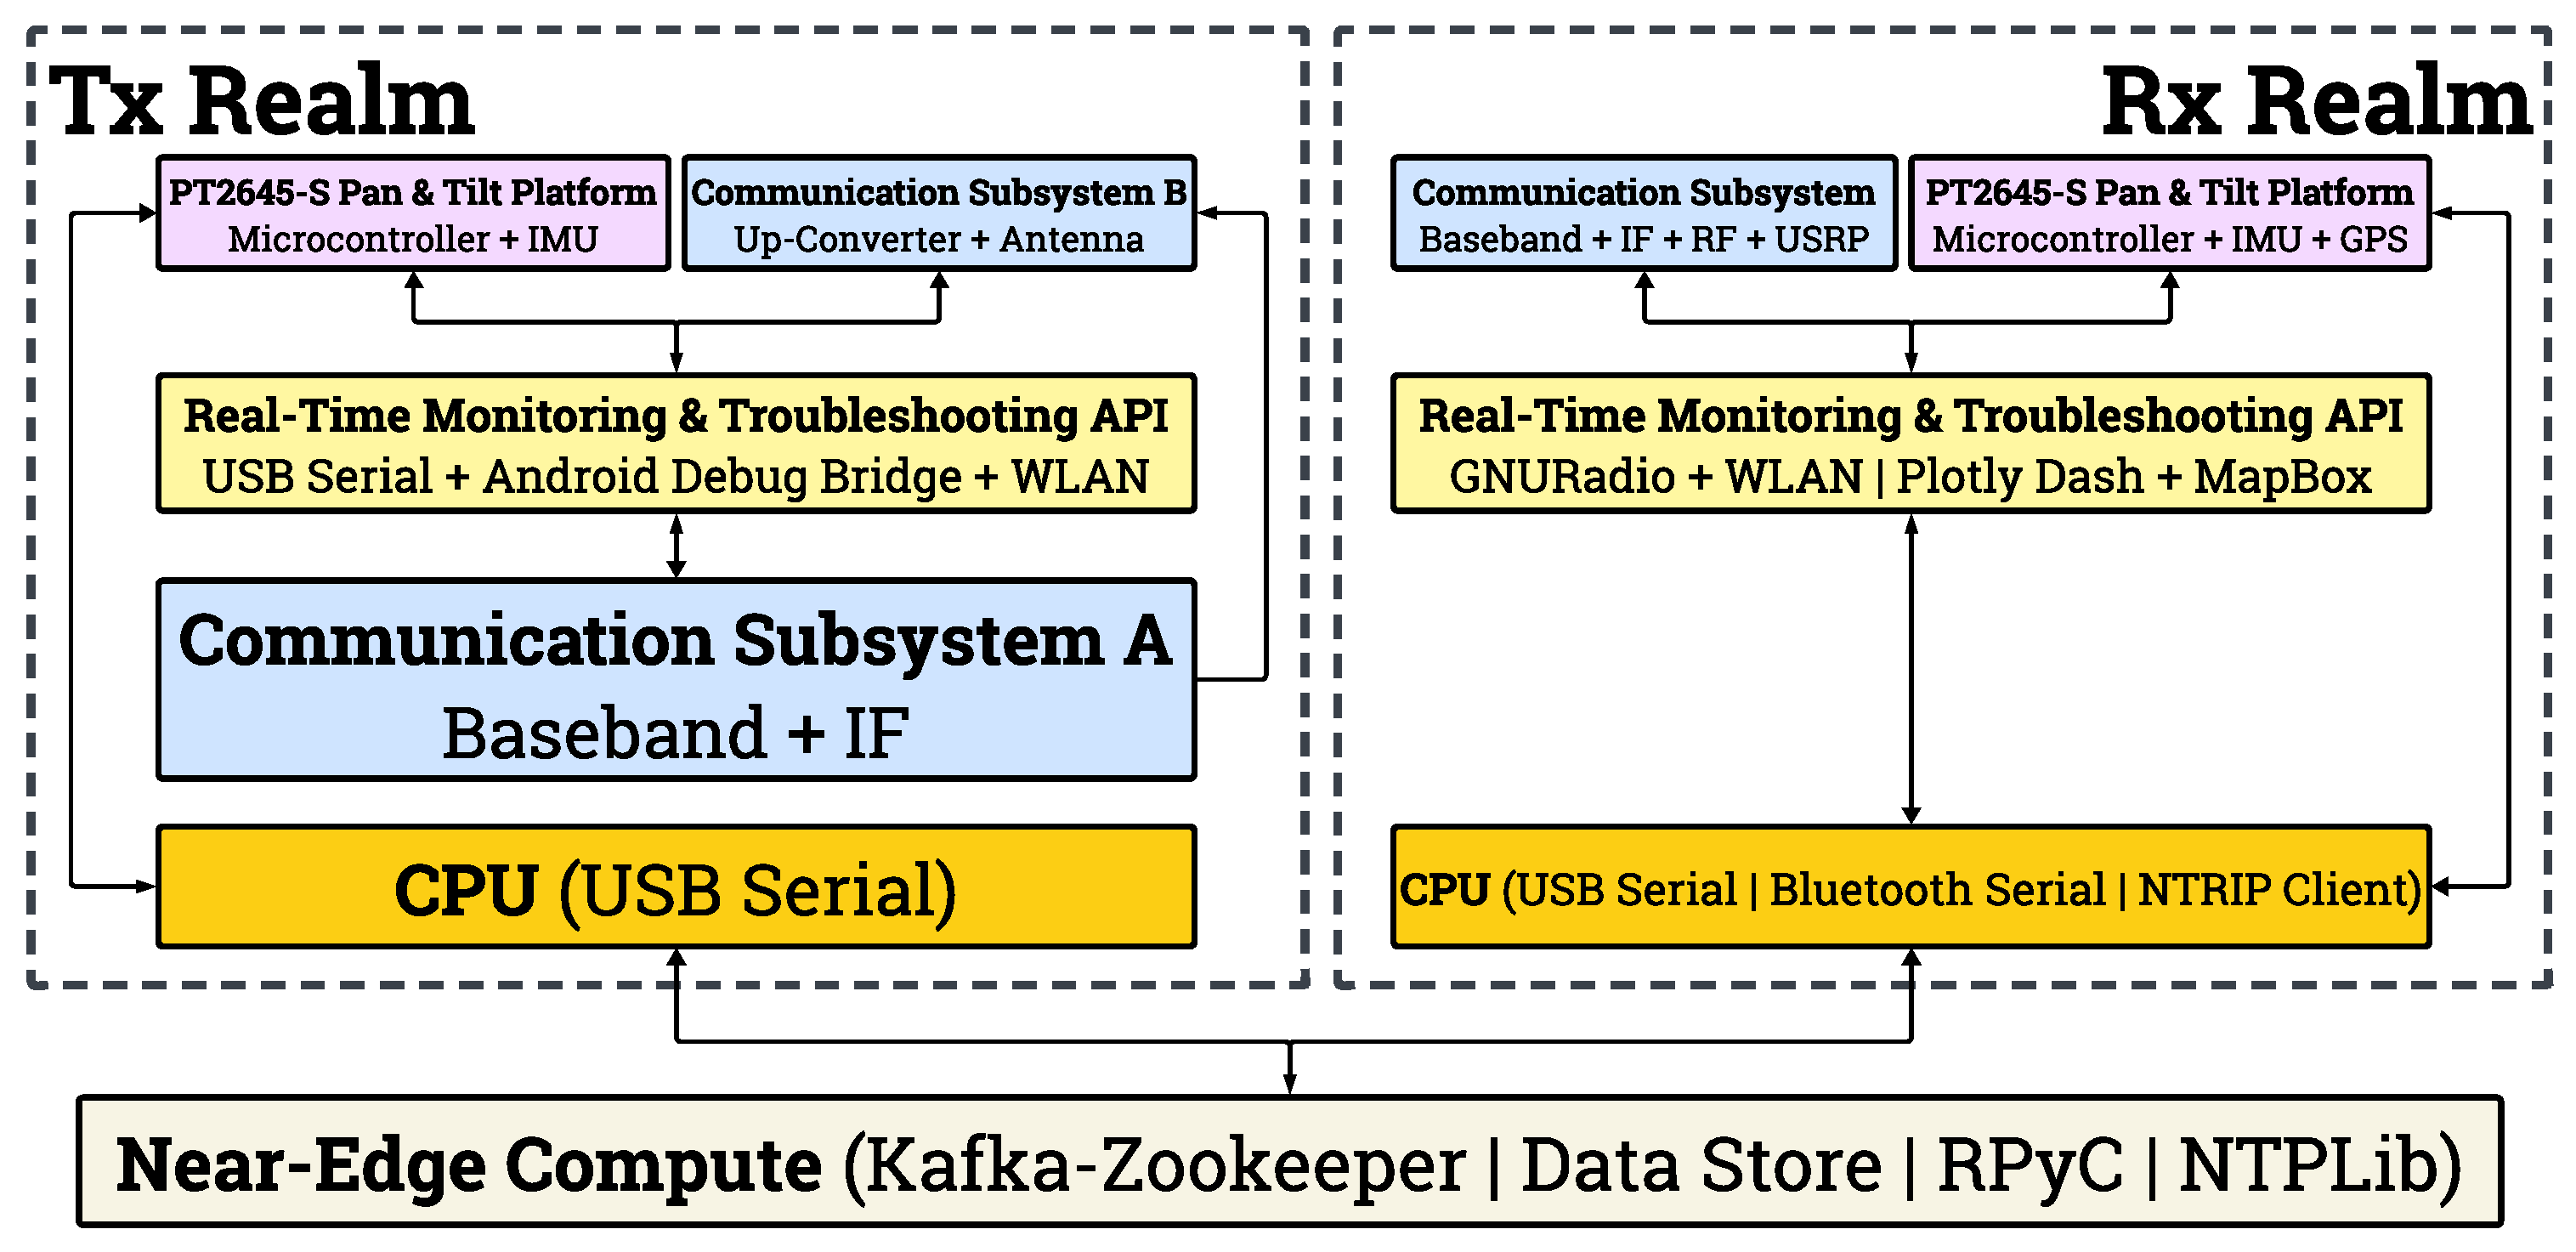
\includegraphics[width=1.0\textwidth]{figs/system_architecture.pdf}
    \vspace{-8mm}
    \caption{The system architecture of our fully-autonomous robotic beam-steering platform with a sliding-correlator channel sounder.}
    \label{F1}
\end{figure*}

\noindent{\textbf{Channel Sounder}}: The measurement system employed a custom broadband sliding-correlator channel sounder at both the Tx and the Rx~\cite{Purdue}, each equipped with a Pseudorandom Noise (PN) sequence generator module producing the required known apriori signal for time-dilated cross-correlation studies, with the Rx module clocked at a slightly lower rate than the Tx; an up-/down-converter to transition between the \SI{2.5}{\giga\hertz} and \SI{28}{\giga\hertz} regimes; a vertically polarized WR-$28$ directional horn antenna; and other commercially available components. This setup is implemented according to the schematics shown in Fig.~\ref{F2a} and Fig.~\ref{F2b}. The operational specifications of the sounder are listed in Table~\ref{T3}, as detailed also in~\cite{Purdue}. As a part of the data-logging operations at the Rx, complex-\SI{64}{} I/Q power delay profiles are recorded onboard an SSD storage drive by a GNURadio sink on a Raspberry Pi SBC via a USRP B$200$mini SDR.
\begin{figure*} [t]
    \centering
    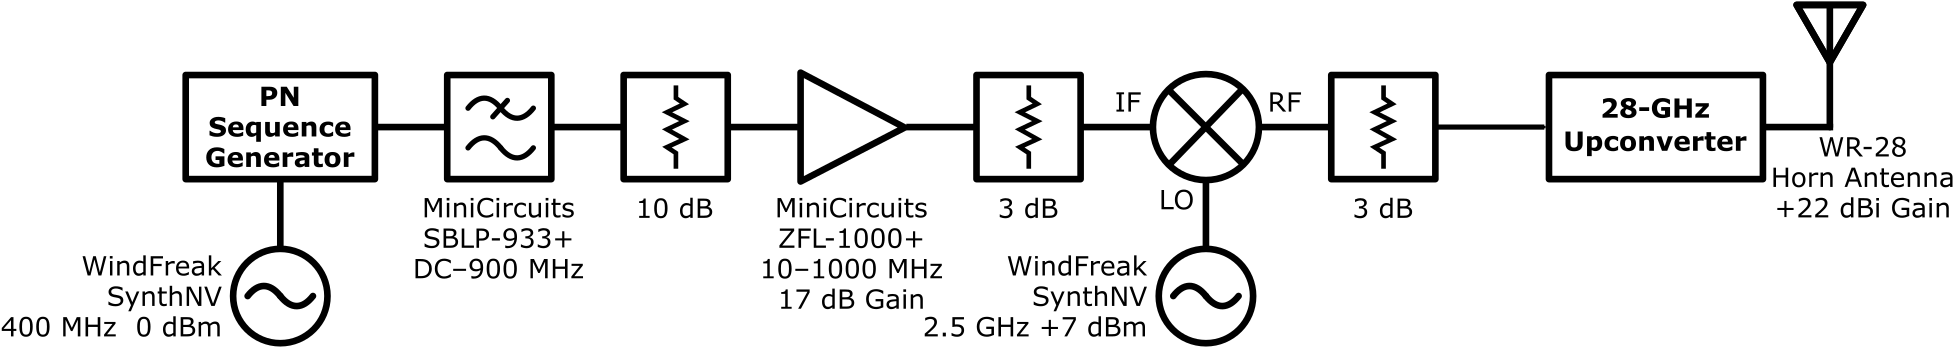
\includegraphics[width=1.0\linewidth]{figs/tx_schematic.png}
    \vspace{-6mm}
    \caption{The Tx circuit schematic with an up-converter, a WR-$28$ horn antenna, and other commercially available components.}
    \label{F2a}
    \vspace{-6mm}
\end{figure*}
\begin{figure*} [t]
    \centering
    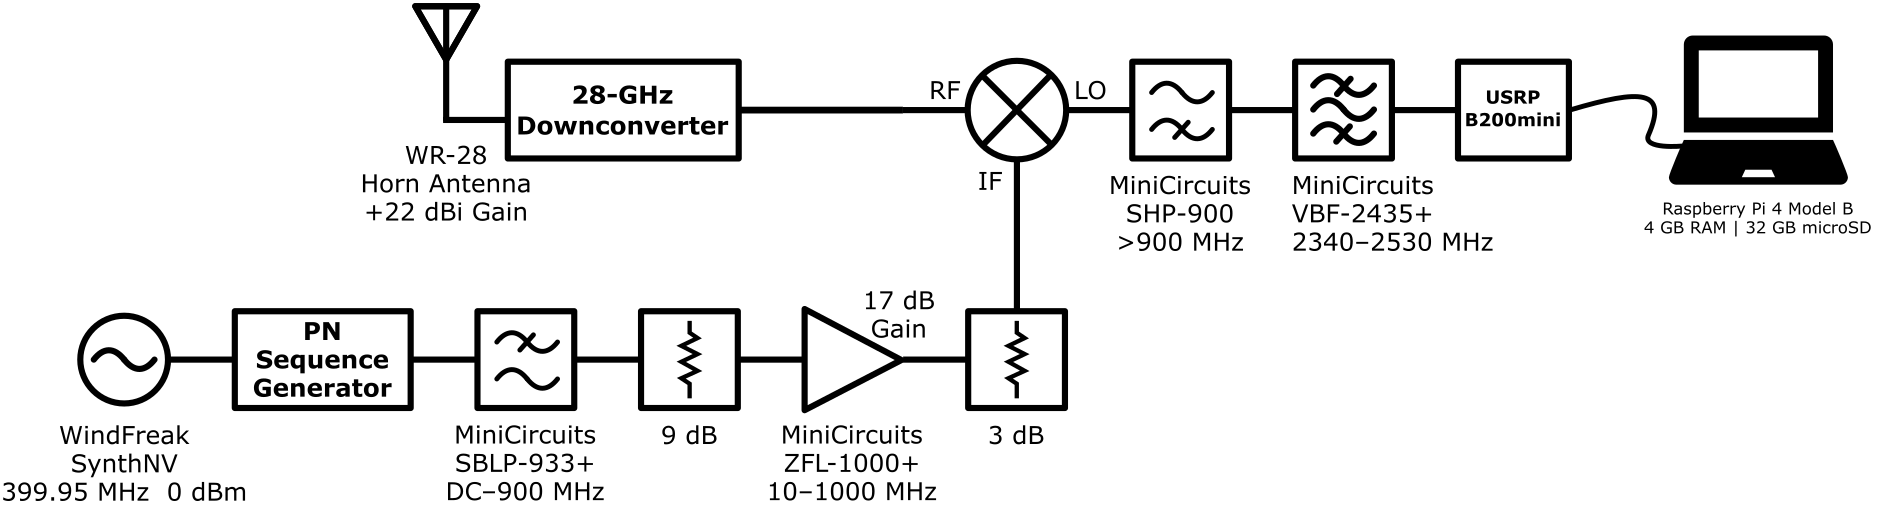
\includegraphics[width=1.0\linewidth]{figs/rx_schematic.png}
    \vspace{-6mm}
    \caption{The Rx circuit schematic with a down-converter, a WR-$28$ horn antenna, and other commercially available components.}
    \label{F2b}
\end{figure*}

\noindent{\textbf{Alignment \& Tracking}}: First, to enable uninhibited rotational mobility for alignment and tracking in the horizontal and the vertical planes, at both the Tx and the Rx, the WR-$28$ horn antenna is mounted on a PT$2645$-S open-loop pan-and-tilt platform, each driven by a pair of HSR-$2645$CRH continuous rotation servos, with each servo actuating either yaw (horizontal) or pitch (vertical) alignment. These servos are controlled via PWM signals from an ATMega$328$P microcontroller with the angular position feedback provided by a BNO$080$ inertial motion unit. This principal axes positioning subsystem demonstrates an average accuracy of \SI{1.1}{\degree} across all fine- \& coarse-grained yaw and pitch movements. Next, for seamless operations in V$2$X scenarios, this alignment platform is augmented with a geo-positioning subsystem consisting of a UBlox GPS ZED-F$9$P unit (with a GNSS multi-band antenna) wherein the positioning accuracy is enhanced by RTCMv$3.0$ RTK correction streams over NTRIP. Demonstrating an average $3$D accuracy of \SI{17}{\centi\meter}, the relevant data members captured by this geo-positioning unit -- namely, the coordinate (latitude, longitude, and ellipsoidal altitude), the horizontal speed \& acceleration, and the heading, are communicated to the microcontroller as NMEA-0183 messages over an I2C serial peripheral bus. A glossary of the acronyms/protocols referenced above is given in Table~\ref{T1}.\\
\renewcommand{\tabcolsep}{6pt}
\begin{table*} [tb]
	\centering
	\scriptsize
	\begin{tabular}{|l||l|}
		\hline
		Carrier Frequency & \SI{28}{\giga\hertz}\\
		\hline
		PN Chip Sequence Length & \SI{2047}{}\\
		\hline
		RF Bandwidth & \SI{800}{\mega\hertz}\\
		\hline
		Tx Chip Rate & \SI{400}{\mega{cps}}\\
		\hline
		Temporal Resolution & \SI{2.5}{\nano\second}\\
		\hline
		Rx Chip Rate & \SI{399.95}{\mega{cps}}\\
		\hline
		Tx Power & \SI{23}{\deci\bel{m}}\\
		\hline
		Tx/Rx Antenna Gain & \SI{22}{\deci\bel{i}}\\
		\hline
		Nominal Tx/Rx Antenna HPBW & \SI{15}{\degree}\\
		\hline
		Measured Tx/Rx Azimuth HPBW & \SI{10.1}{\degree}\\
		\hline
		Measured Tx/Rx Elevation HPBW & \SI{11.5}{\degree}\\
		\hline
		Maximum Measurable Pathloss & \SI{182}{\decibel}\\
		\hline
		GNURadio Sink Center Frequency & \SI{2.5}{\giga\hertz}\\
		\hline
		USRP Gain & \SI{76}{\decibel}\\
		\hline
		USRP Sampling Rate & \SI{2}{\mega{sps}}\\
		\hline
	\end{tabular}
	\vspace{-1mm}
	\caption{The specifications of the sliding-correlator channel sounder used in our measurement campaign on NSF POWDER.}
	\label{T3}
\end{table*}
\indent{Since} our measurement system revolves around a decoupled design with the alignment and tracking platform replicated at both the Tx and the Rx, a centralized nerve-center handles asynchronous module registration \& de-registration via RPyC object proxying, global timing synchronization via NTP, and coordination between the Tx and Rx over fault-tolerant Apache Kafka messaging middleware. With an Apache Zookeeper broker manager serving as a distributed configuration, synchronization, and naming registry service for the Kafka cluster, the samples generated by the principal axes positioning and geo-positioning subsystems are shared over Kafka message queues (known as topics, e.g., "SPAVE\_$28$G\_RX\_GPS\_EVENTS"): the Tx subscribes to the alignment and geo-location messages published by the Rx, and vice-versa, resulting in a scalable event-driven modular architecture. Corroborated both onsite and in the laboratory, this publish-subscribe framework facilitates an average beam-steering response time of \SI{27.8}{\milli\second}, evaluated over ${\approx}$\SI{13000}{} interactions. With system monitoring provided over an Android debug bridge and system troubleshooting enabled via serial communication interfaces, our platform demonstrates remote orchestration capabilities: a critical necessity for mmWave propagation modeling in V$2$X settings. To augment these remote monitoring and troubleshooting features further, a GNURadio Qt GUI time-sink (with dynamic trigger levels) allows for real-time visualization of the recorded power delay profiles over an ad-hoc WLAN with the Raspberry Pi SBC; additionally, via the Plotly Dash and MapBox APIs, the Tx and Rx geo-locations are annotated with their relative alignment accuracies and visualized in real-time for onsite validation of the routes traversed on the NSF POWDER experimental testbed in Salt Lake City, UT.
\vspace{-3mm}

% Measurement campaign description and Data post-processing procedural explanation
\section{Measurements \& Post-Processing}\label{S3}
In this section, we discuss the operations involved in our \SI{28}{\giga\hertz} V$2$X measurement campaign on the NSF POWDER testbed. First, we describe the system calibration process, after which we outline the onsite system deployment procedure. Subsequently, we detail the post-processing steps involved in setting up the power delay profiles recorded at the Rx for pathloss evaluations including the empirical verifications of mmWave UMa and UMi pathloss standards; multipath component extraction and parameter estimation via the SAGE algorithm~\cite{SAGE}; spatial consistency analyses vis-\`{a}-vis Tx-Rx distance, alignment accuracy, and relative velocity; multipath clustering analyses; Doppler shift and small-scale fading studies; and mmWave channel model validations.

\noindent{\textbf{Pre-deployment Calibration}}: After the Tx and Rx circuits for the sliding-correlator channel sounder have been implemented as illustrated in Fig.~\ref{F2a} and Fig.~\ref{F2b}, a calibration procedure is carried out onsite to map the power calculated from the power delay profiles recorded by the USRP to reference measured power levels. The process of calibrating the measurement system before deployment ensures accurate Rx power calculations in the presence of imperfect circuit components, e.g., the Commscope LDF$4$-$50$A \SI{0.5}{{"}} coaxial cables employed at the Tx exhibit losses of up to \SI{0.12}{\deci\bel\per\meter} at \SI{2.5}{\giga\hertz}. Under \SI{0}{\deci\bel} and \SI{76}{\deci\bel} USRP gains, using a Keysight variable attenuator, the recorded power delay profiles are processed to determine the calculated power values mapped to their corresponding reference power levels: the results of this procedure are employed in our numerical evaluations detailed in Sec.~\ref{S4} and Sec.~\ref{S5}~\cite{SPAVE_ICC}. We discuss the deployment of our measurement system onsite at the NSF POWDER experimental testbed next.

\noindent{\textbf{NSF POWDER Deployment}}: As described in Sec.~\ref{S2}, our measurement system assembly constitutes an autonomous beam-steering controller replicated at both the Tx and the Rx, their respective sounder circuits, and a centralized nerve center for aggregation (via RPyC), timing synchronization (via NTP), and coordination (via Kafka-Zookeeper). On the NSF POWDER testbed, the nerve center is deployed on a high-availability cluster of four Dell R$740$ compute nodes at the Fort Douglas datacenter, with fault tolerance being a key feature to ensure storage redundancy for the recorded data. As depicted in Fig.~\ref{F3a}, the Tx is mounted on a building rooftop; while, as shown in Fig.~\ref{F3b}, the Rx is mounted on a van (or a push-cart) that is driven (or pushed) along unplanned routes onsite. Remote monitoring and troubleshooting is provided for validation of geo-positioning, alignment, and power delay profile samples. The goal of this measurement campaign was to obtain a reasonably large dataset of site-specific measurements for evaluating the propagation characteristics of \SI{28}{\giga\hertz} signals in vehicular communication settings. Thus, our propagation modeling activities included V$2$I measurements under manual, semi-, and fully-autonomous alignment operations traversing nine routes spanning urban, suburban, and foliage environments. Although our platform is capable of double-directional measurements and facilitates easy scalability to MIMO settings, in this paper, we focus only on beam-steered measurements in V$2$X settings -- particularly for spatial decoherence studies, multipath clustering evaluations under LoS/OLoS link scenarios, and Doppler shift and small-scale fading analyses.
\begin{figure*}[t]
    \centering
     \begin{subfigure}{0.355\linewidth}
         \centering
         \includegraphics[width=1.0\linewidth]{figs/tx_deployment.pdf}
         \caption{Tx Deployment at Browning}
         \label{F3a}
     \end{subfigure}
     \begin{subfigure}{0.635\linewidth}
         \centering
         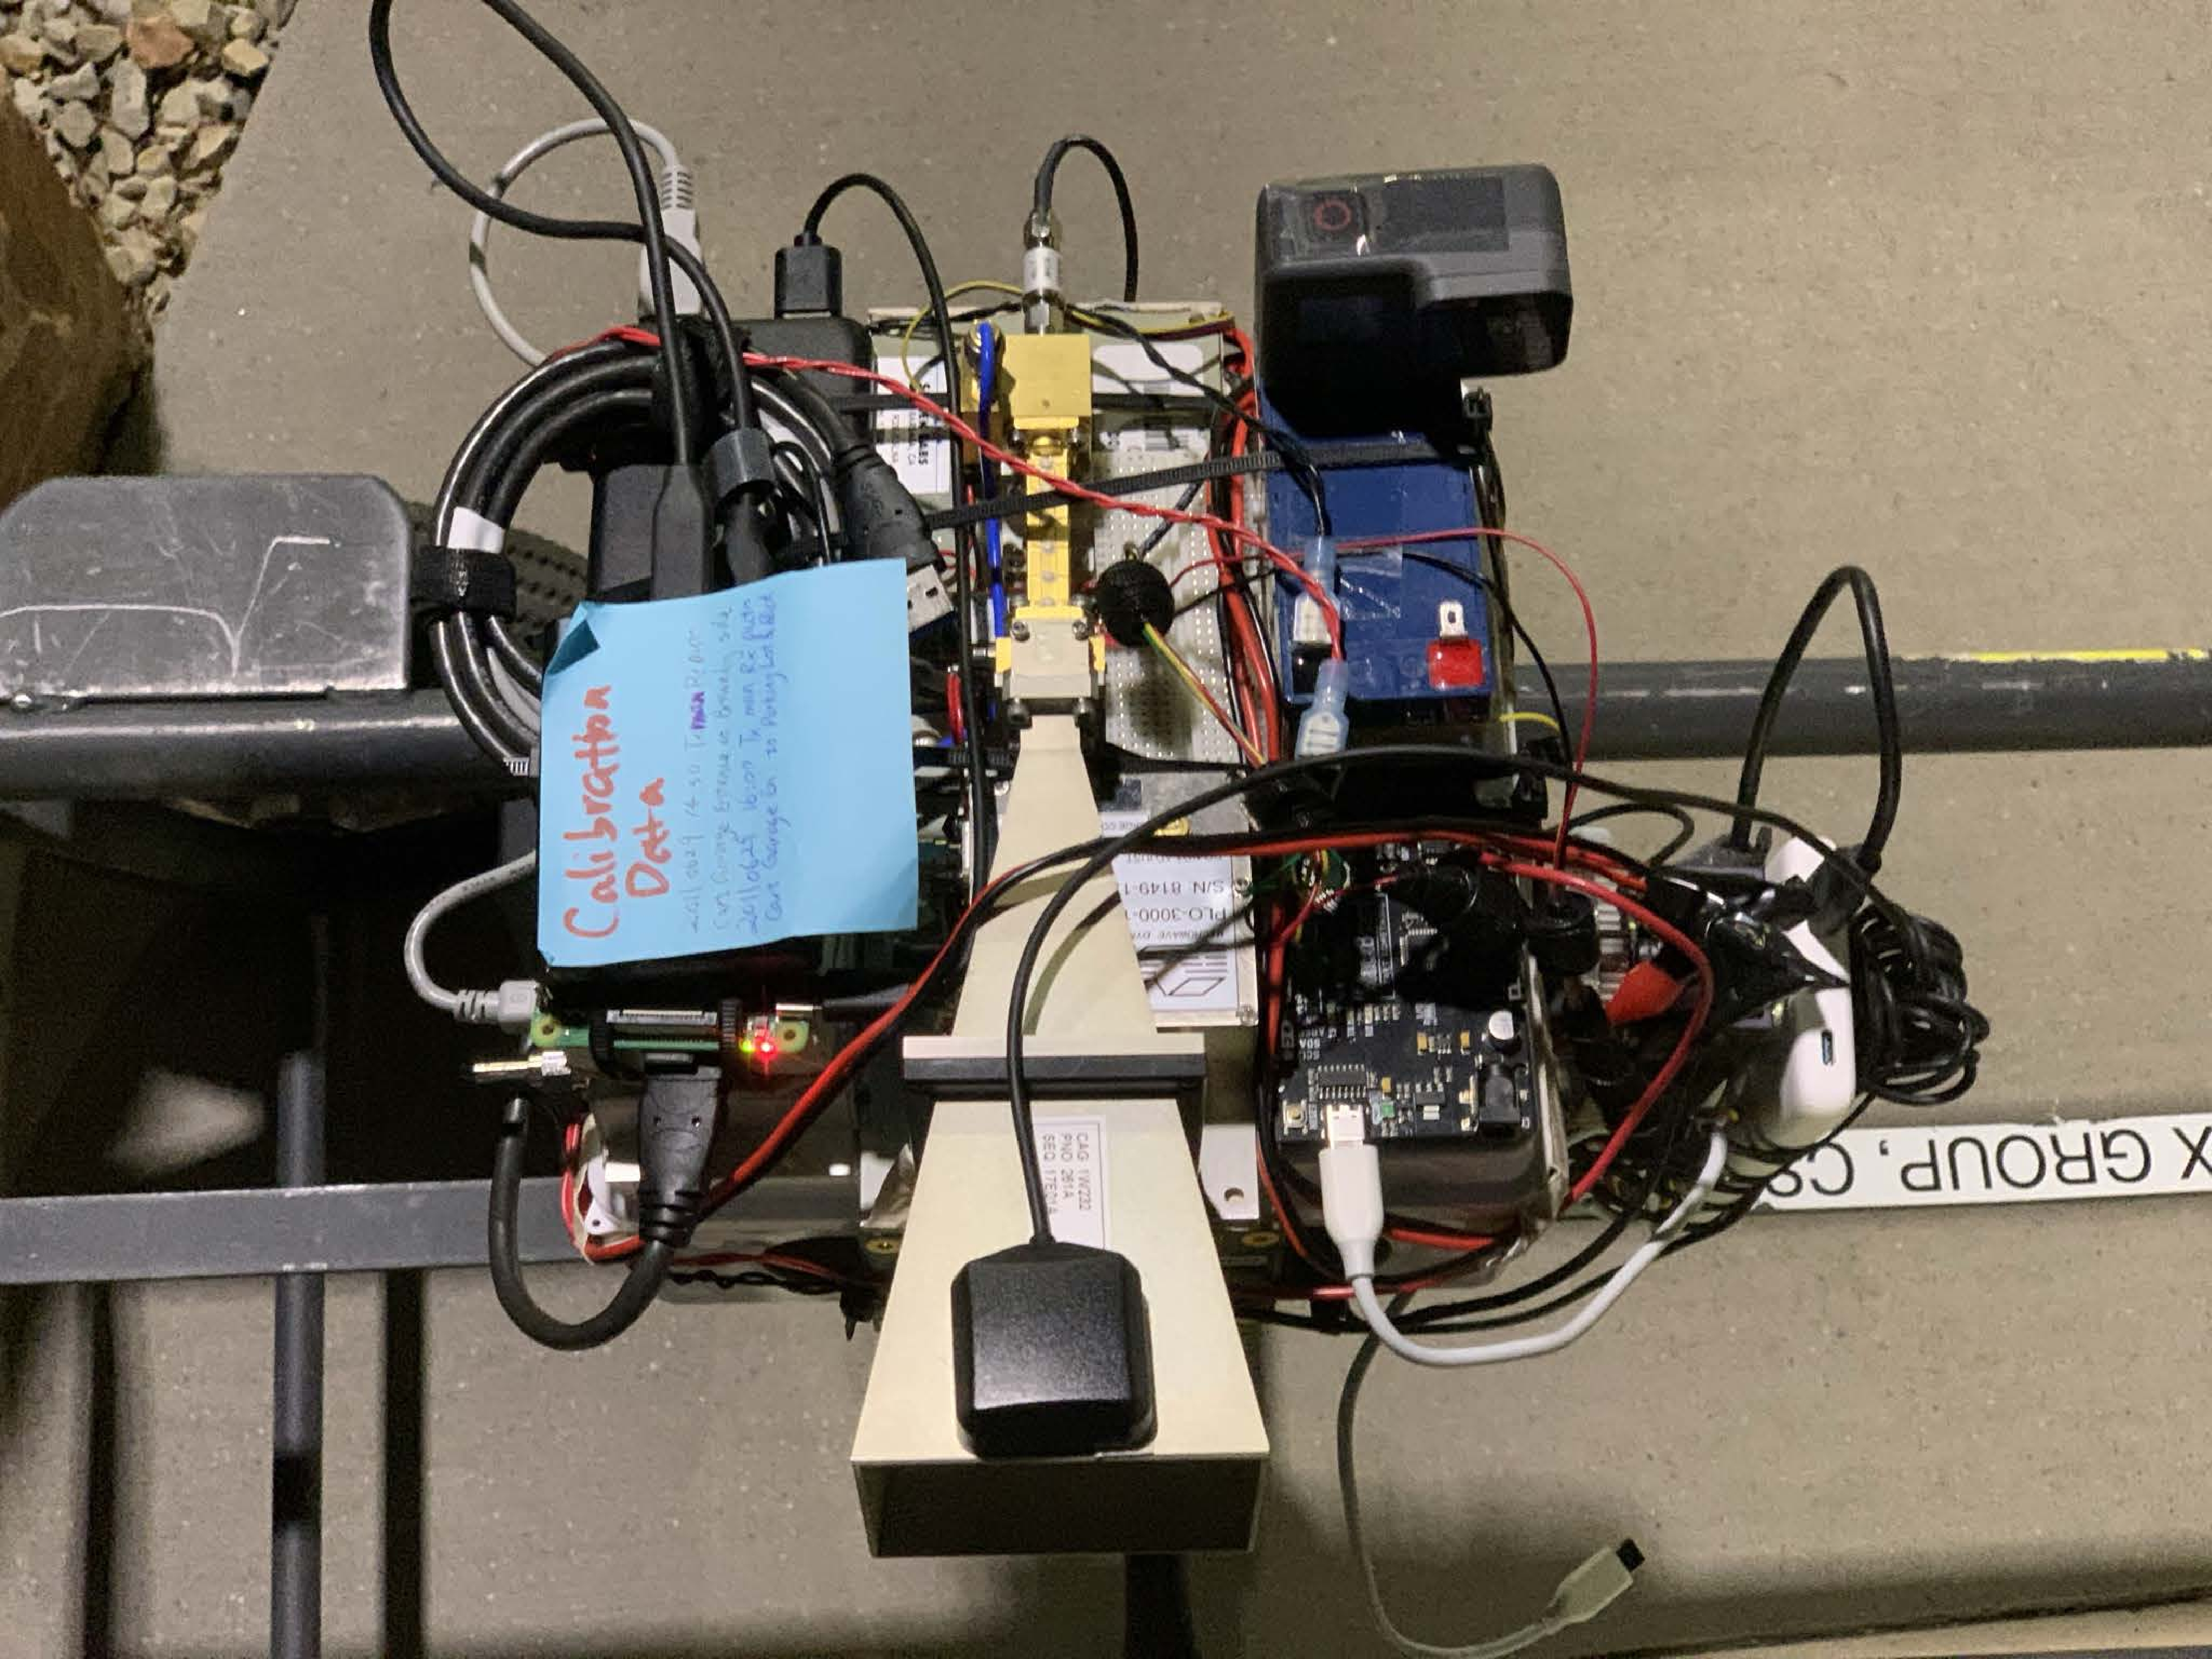
\includegraphics[width=1.0\linewidth]{figs/rx_deployment.pdf}
         \caption{Rx Cart Deployment}
         \label{F3b}
     \end{subfigure}
     \vspace{-8mm}
    \caption{The Tx deployment atop the William Browning building, where the sounder circuits are housed in a climate-controlled enclosure with the antenna mounted on the pan-and-tilt platform (a); and the Rx deployment on a push-cart (or a minivan) (b).}
    \label{F3}
\end{figure*}

\noindent{\textbf{{Post-Processing}}: Using GNURadio utilities, the metadata file corresponding to the route-specific power delay profile records at the Rx is parsed to extract timestamp information, which is then associated with the geo-positioning and alignment logs at both the Tx and the Rx. The samples in each synchronized power delay profile segment undergo pre-filtering via a low-pass filter (SciPy FIR implementation), time-windowing, and noise-elimination (via a custom peak-search and subsequent thresholding mechanism). Coupled with transmission power and antenna gain values, the received power levels obtained from these processed samples allow the visualization of pathloss maps on the Google Maps API (rendered via the Bokeh toolbox), and the evaluation of pathloss behavior as a function of Tx-Rx distance, with validations against the $3$GPP TR$38.901$, ITU-R M$.2135$, METIS, and mmMAGIC standards~\cite{MacCartneyModelsOverview}. The SAGE algorithm~\cite{SAGE} is used to extract multipath parameters, which facilitates RMS delay- and direction-spread studies~\cite{Indoor60G}. Under variations in Tx-Rx distance, Tx-Rx alignment accuracy, and Tx-Rx relative velocity, we probe signal decoherence patterns via the spatial autocorrelation coefficient~\cite{MacCartneySpatialStatistics}. Additionally, investigating the extracted multipath components in further detail facilitates analyses on their clustering characteristics at the Rx, viz., their inter-arrival times, their peak-power distributions, and their decay attributes; also, these multipath components enable the visualization of Power Delay Angular Profiles (PDAPs) along different routes for insights into the site-specific temporal \& spatial dispersion features of \SI{28}{\giga\hertz} signals. The visualizations of Power Delay Doppler Profiles (PDDPs) and normalized Doppler spectra along the various routes traversed onsite during the measurement campaign shed light on the Doppler shift properties of the signals in V$2$X settings; moreover, pathloss versus time studies for specific routes dominant in  dynamic blockages (pedestrians and moving/parked vehicles) allow examinations of the small-scale fading attributes of mmWave signals: specifically, the average fade-depth and the average fade-duration. Lastly, these investigations facilitate validations of popular channel models -- namely, Saleh-Valenzuela (SV), Quasi-Deterministic (QD), Device-to-Device (D$2$D), and stochastic channel models.
\vspace{-3mm}

% Numerical evaluations I: Pathloss studies and Spatial consistency evaluations
\section{Pathloss and Spatial Consistency Evaluations}\label{S4}
In this section, we outline the initial set of results derived from our evaluations on the collected datasets. We first briefly study the radiation patterns of the directional horn antennas and the results of our calibration procedure, both of which are then employed in our ensuing evaluations; next, we analyze the empirical pathloss results attained from our measurements along a diverse set of routes and validate them against popular outdoor pathloss standards; additionally, we outline the insights obtained from our shadow fading investigations under the effects of static geometry-induced losses; subsequently, we detail our spatial consistency evaluations and examine the resultant plots vis-\`{a}-vis Tx-Rx distance, alignment accuracy, and relative velocity; finally, we describe our findings on the small-scale fading attributes of \SI{28}{\giga\hertz} signals in V$2$X applications, in addition to their comparisons with state-of-the-art D$2$D mmWave statistical channel model. 

\noindent{\textbf{Antenna Patterns \& Calibration}}: Obtained via empirical recordings of the WR-$28$ antenna's operational characteristics, Fig.~\ref{F4a} and Fig.~\ref{F4b} illustrate its $2$D radiation patterns along the azimuth and elevation directions, respectively: these enable us to compute the gains at specific locations along a route and at specific degrees of alignment, crucial for our subsequent analyses. As evident from these radiation pattern illustrations, the WR-$28$ horn antennas employed in our propagation modeling campaign are highly-directional, thus necessitating the need for an accurate and reliable beam-steering system, particularly in V$2$X measurement scenarios. Furthermore, conducting the pre-deployment calibration procedure as outlined in Sec.~\ref{S3}, we derive a linear relationship between the measured received power levels and their calculated power values corresponding to artificial attenuation injections into the signal path between the Tx and the Rx. This calibration relationship (for both \SI{0}{\deci\bel} and \SI{76}{\deci\bel} USRP gain values) allows us to account for losses introduced into our measurements due to imperfect circuit components: refer to the preliminary manuscript of our research efforts for illustrations and additional details~\cite{SPAVE_ICC}.
\begin{figure*} [t]
     \centering
     \begin{subfigure}{0.494\linewidth}
         \centering
         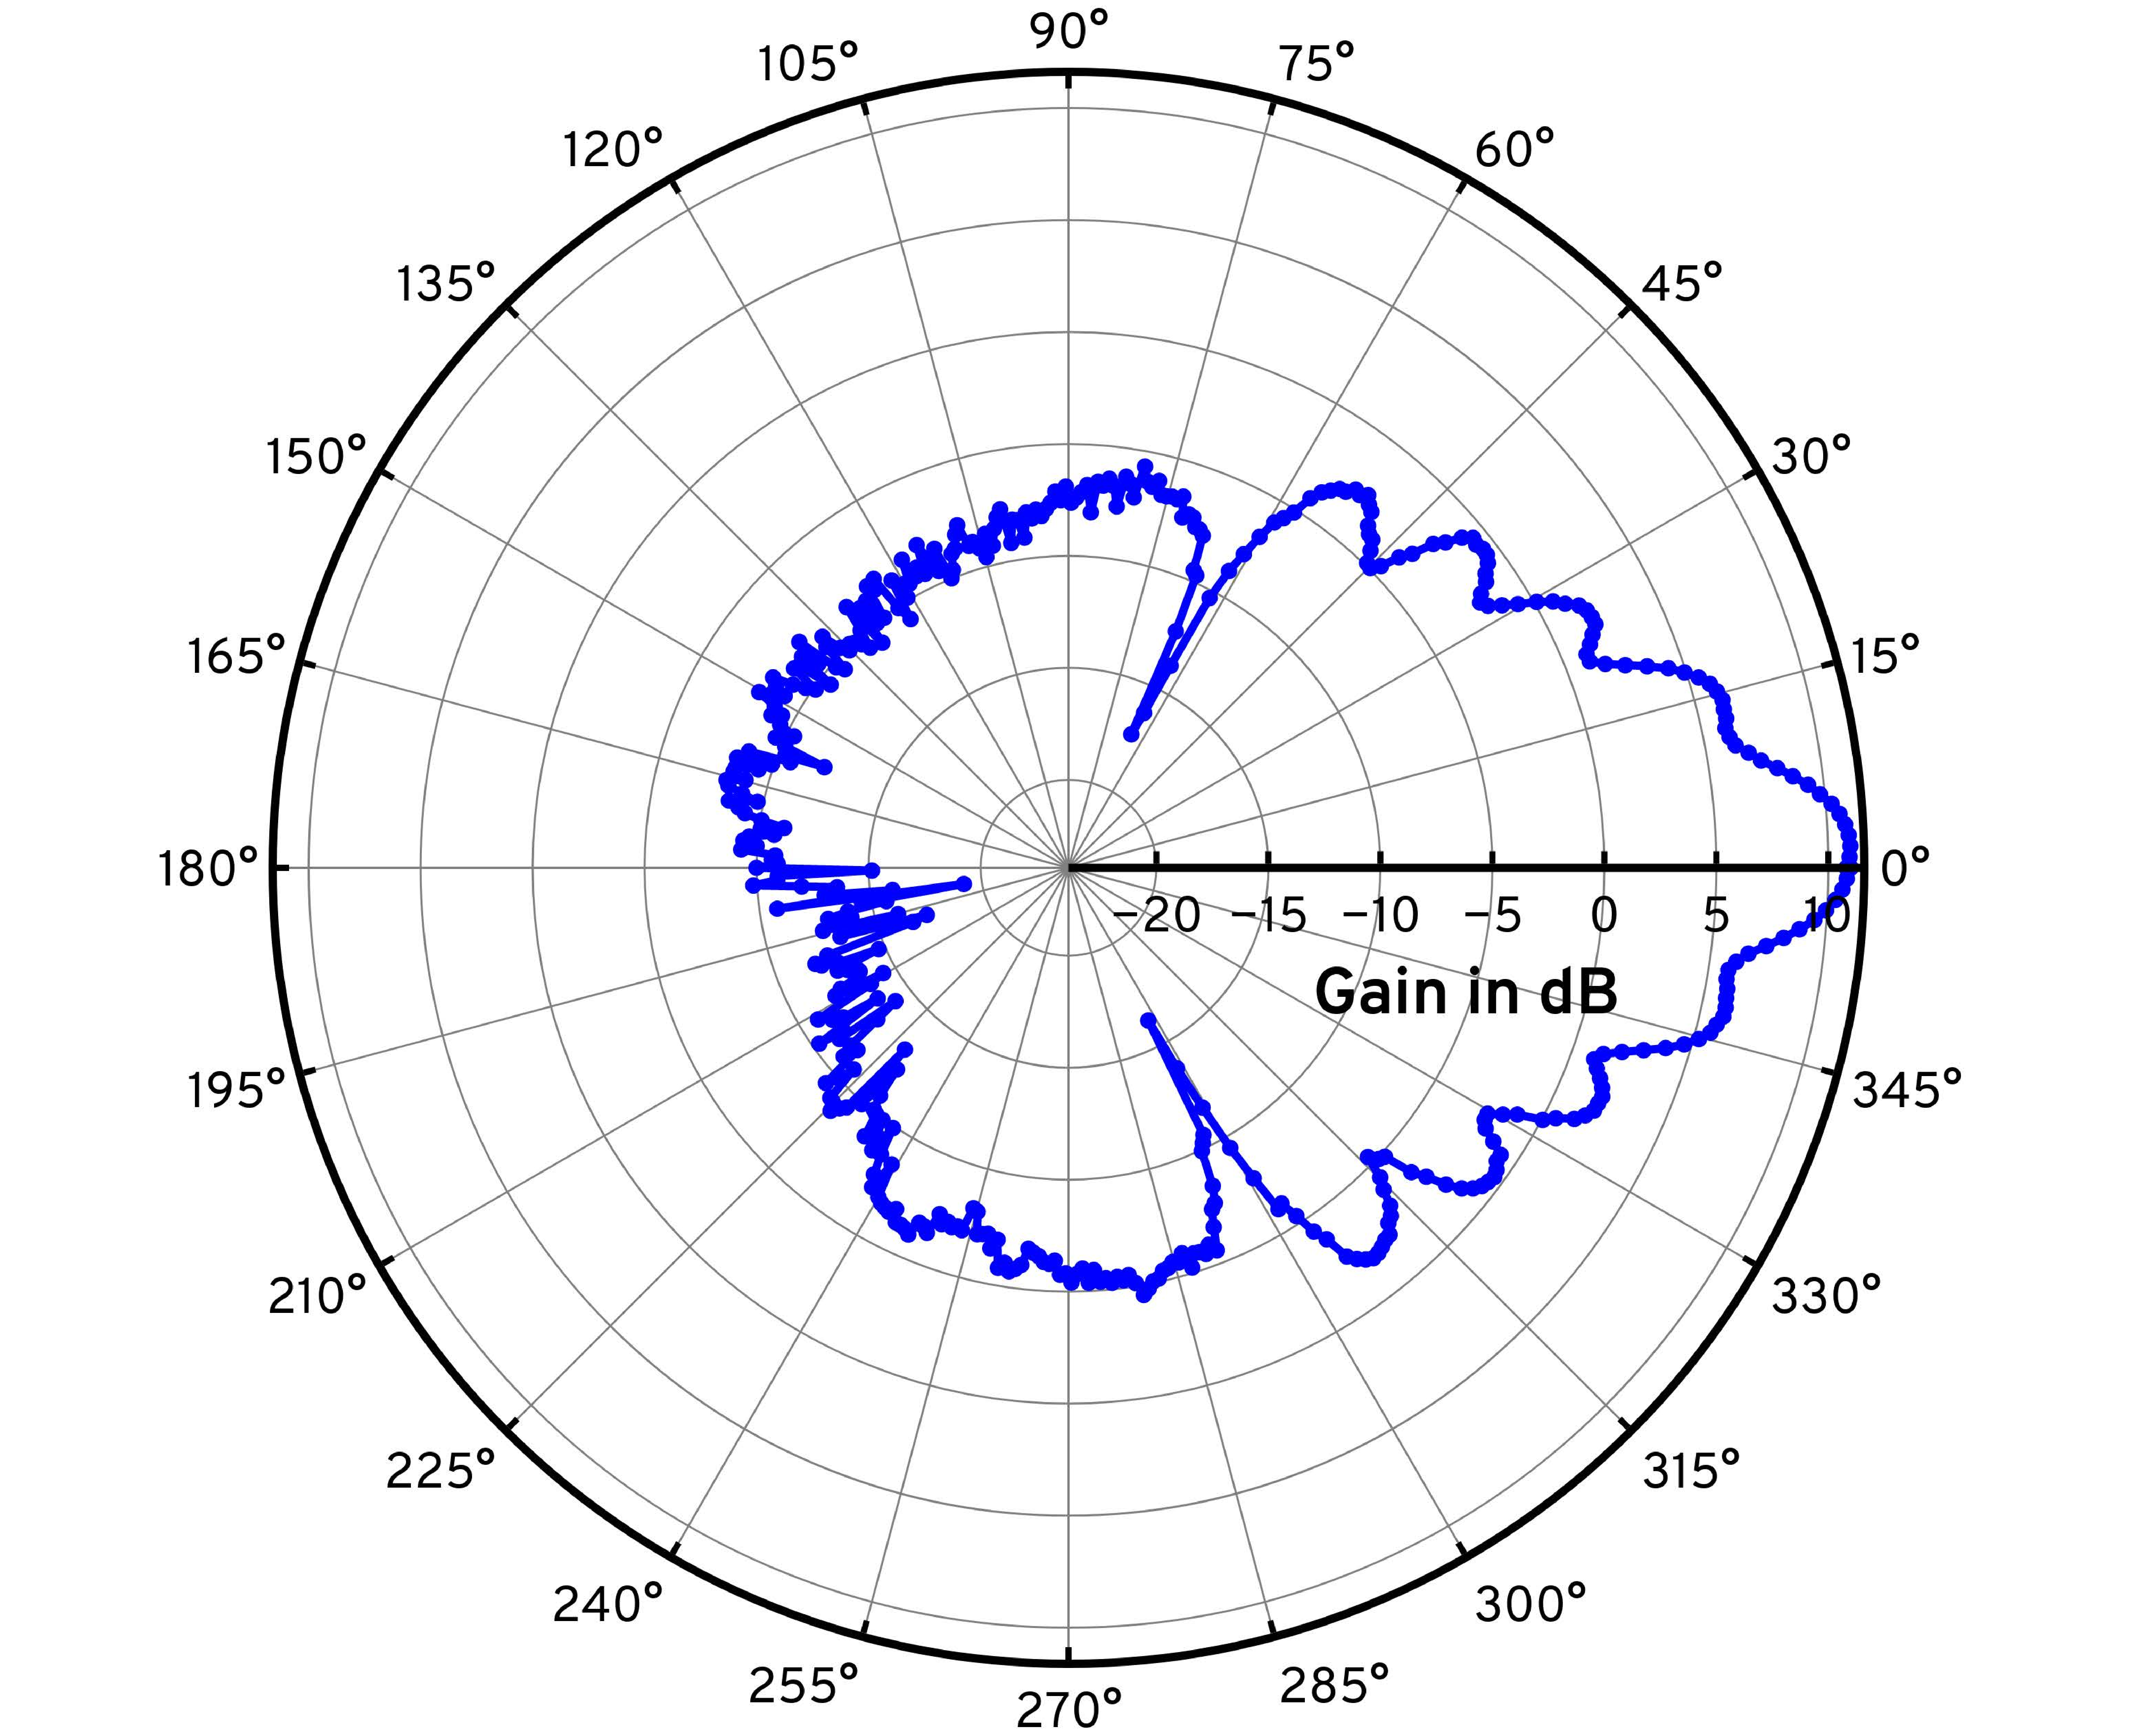
\includegraphics[width=1.0\linewidth]{figs/antenna_pattern_az.pdf}
         \caption{Antenna Pattern (Azimuth)}
         \label{F4a}
     \end{subfigure}
     \begin{subfigure}{0.496\linewidth}
         \centering
         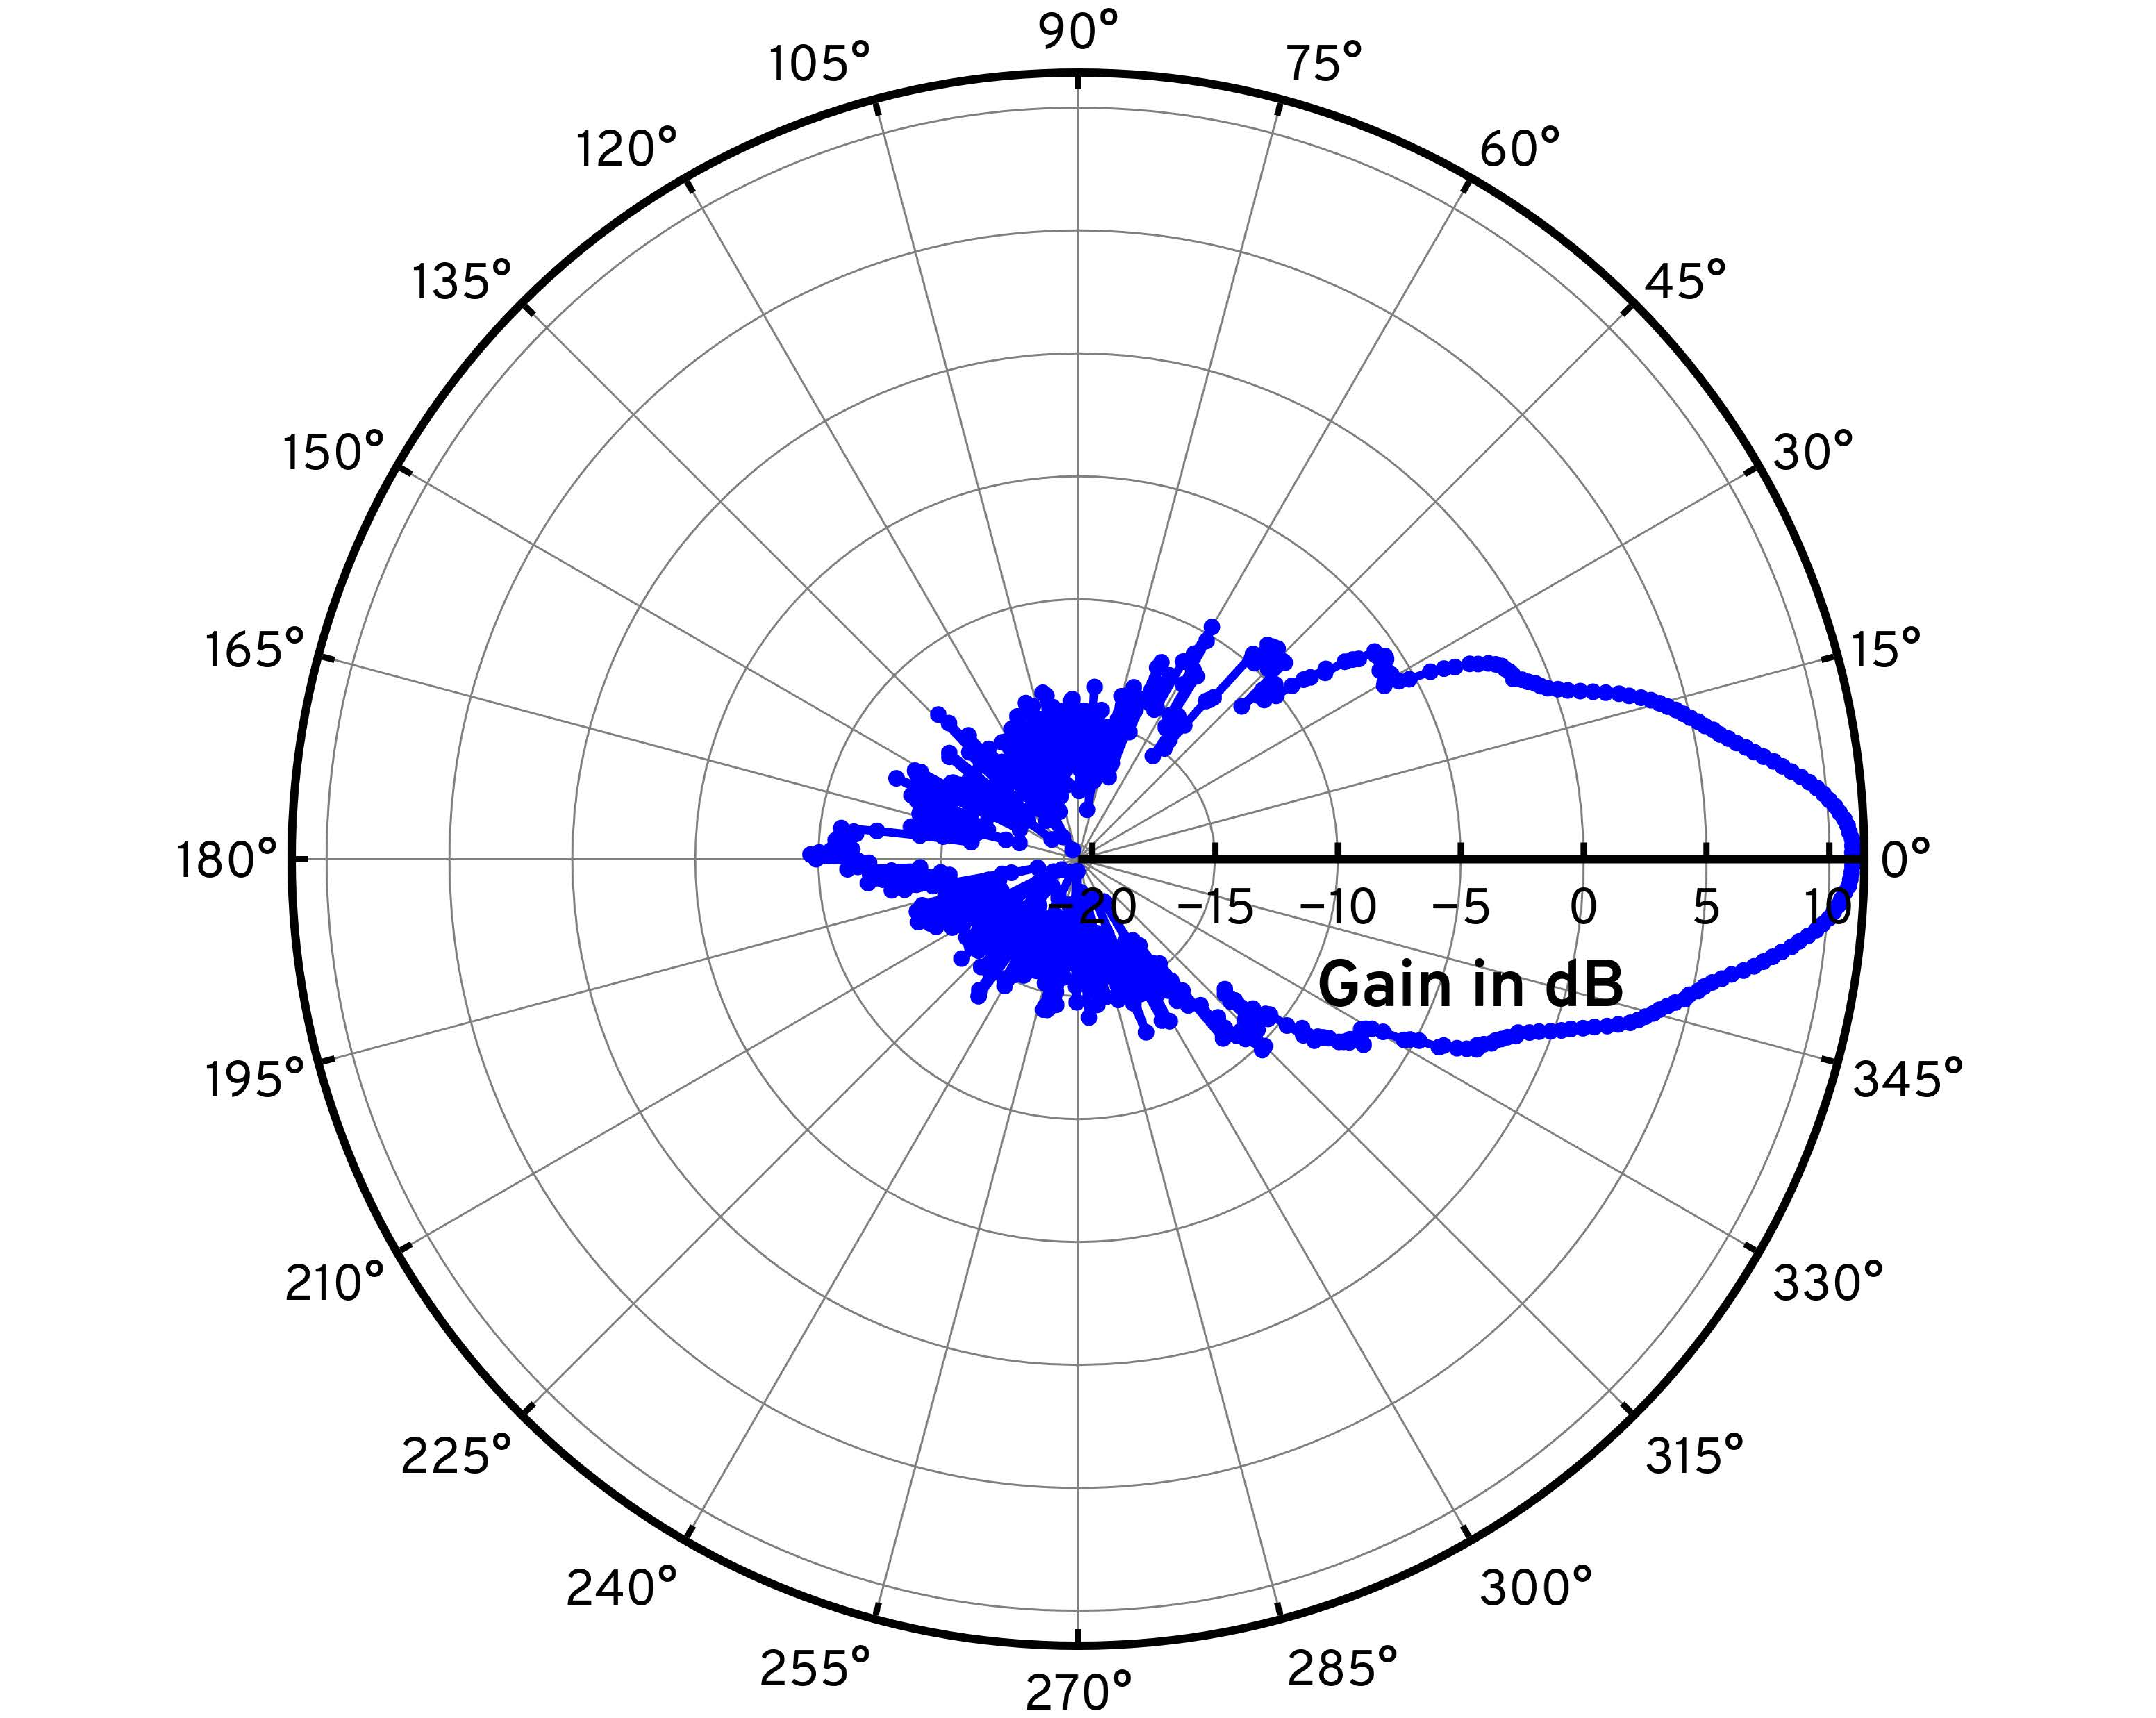
\includegraphics[width=1.0\linewidth]{figs/antenna_pattern_el.pdf}
         \caption{Antenna Pattern (Elevation)}
         \label{F4b}
     \end{subfigure}
     \vspace{-8mm}
     \caption{The normalized measured $2$D radiation patterns along the azimuth (a) and elevation (b) directions for the WR-$28$ antennas.}
     \label{F4}
\end{figure*}

\noindent{\textbf{Pathloss Studies}}: Upon post-processing the collected measurements (GPS logs, IMU samples, and power delay profiles) according to the processing operations detailed in Sec.~\ref{S3}, we compute the signal power at the Rx (with calibration offsets); subsequently, knowing the Tx power and the antenna gains, we compute the pathloss experienced at each Rx position along a specific route onsite. Fig.~\ref{F5a} and Fig.~\ref{F5b} depict the pathloss heat-maps (superimposed on Google Hybrid maps) for the urban campus routes traversed during our measurement campaign -- namely, the route around President's Circle and the route around 100 S St, respectively. With the Tx affixed atop the William Browning building, for the urban campus route around President's Circle (Fig.~\ref{F5a}), the Rx was mounted on a minivan and driven around onsite, while for the urban campus route around 100 S St (Fig.~\ref{F5b}), the Rx was mounted on a cart and pushed around onsite. It is evident from these pathloss heatmaps in Fig~\ref{F5a} and Fig.~\ref{F5b} that the received signals along the 100 S St route (Fig.~\ref{F5b}) as opposed to those along the President's Circle route (Fig.~\ref{F5a}) experience relatively lower pathloss due to their comparatively smaller Tx-Rx distances and smaller Tx-Rx relative velocities (cart vs van). Also, note that in Fig.~\ref{F5b}, since at certain locations, the Rx is hidden behind tall buildings, the obstacle-induced losses (i.e., shadow fading) have a dominant impact on the received signal strength: this is discussed in further detail later in this section. Similarly, Fig.~\ref{F6a} and Fig.~\ref{F6b} depict the pathloss heat-maps (superimposed on Google Hybrid maps) of the foliage-dominated route (campus vegetation around the Olpin Union building) and the suburban neighborhood route (around S Wolcott St), respectively. With the Tx affixed atop the William Browning building, for both these routes, the Rx is mounted on a cart and pushed around onsite. Evaluating the differences in received signal power trends between these two routes, we observe that, across similar Tx-Rx distances, the foliage-dominated environment (Fig.~\ref{F6a}) as opposed to the suburban environment with a considerably lower vegetation density (Fig.~\ref{F6b}) presents larger pathloss due to the foliage-induced diffractions introduced into the signal propagation path.
\begin{figure*} [t]
     \centering
     \begin{subfigure}{0.563\linewidth}
         \centering
         \includegraphics[width=1.0\linewidth]{figs/urban_campus_pathloss_1.pdf}
         \caption{Urban Campus (President's Circle)}
         \label{F5a}
     \end{subfigure}
     \begin{subfigure}{0.427\linewidth}
         \centering
         \includegraphics[width=1.0\linewidth]{figs/urban_campus_pathloss_2.pdf}
         \caption{Urban Campus (100 S St)}
         \label{F5b}
     \end{subfigure}
     \vspace{-8mm}
     \caption{The pathloss values superimposed on a Google Hybrid map for the urban campus routes onsite: President's Circle (the Rx is on a minivan) and 100 S St (the Rx is on a push-cart). Here, the heat-map color palette dots denote the Rx positions along the route, while the blue diamond denotes the fixed Tx location atop the William Browning building.}
     \label{F5}
\end{figure*}

Ensuing these heat-map illustrations of the pathlosses experienced by \SI{28}{\giga\hertz} signals around the various routes traversed onsite, we compare the pathloss versus distance behavior of mmWave signals in our measurement campaign with outdoor micro- and macro-cellular pathloss standards ($3$GPP TR$38.901$, ITU-R M$.2135$, METIS, and mmMAGIC~\cite{MacCartneyModelsOverview}). These popular standards constitute both line-of-sight and non-line-of-sight models, with a Tx height of $h_{\text{Tx}}{\approx}$\SI{25}{\meter} and a Tx-Rx $2$D separation range of \SI{10}{\meter}${\leq}d_{2\text{D}}{\leq}$\SI{5000}{\meter}, which match the deployment specifications of our campaign, making them suitable candidates for empirical validations. In particular, as shown in Fig.~\ref{F7a}, evaluating the pathlosses computed from our collected measurements against these standards for the urban campus (President's Circle and 100 S St), suburban neighborhood (S Wolcott St), and foliage environment (Olpin Union) routes, we observe that all these pathloss standards fail to accurately capture the pathloss versus log-distance behavior of \SI{28}{\giga\hertz} signals in V$2$X propagation scenarios. Specifically, we notice that, employing a linear-curve fitting procedure (via a floating intercept model) to extrapolate the pathloss values across an extended range of Tx-Rx distances (solid lines for our measurements and dashed lines for the subsequent extrapolation), there is a significant discrepancy between our measurements and the standards in the characteristics of the pathloss across such distances. Therefore, we can conclude that the $3$GPP TR$38.901$, ITU-R M$.2135$, METIS, and mmMAGIC large-scale outdoor pathloss standards require considerable improvements to account for mmWave propagation in V$2$X applications.
\begin{figure*} [t]
     \centering
     \begin{subfigure}{0.557\linewidth}
         \centering
         \includegraphics[width=0.9\linewidth]{figs/foliage_pathloss.pdf}
         \caption{Foliage Environment (Olpin Union)}
         \label{F6a}
     \end{subfigure}
     \begin{subfigure}{0.433\linewidth}
         \centering
         \includegraphics[width=0.9\linewidth]{figs/suburban_pathloss.pdf}
         \caption{Suburban Neighborhood (S Wolcott St)}
         \label{F6b}
     \end{subfigure}
     \vspace{-8mm}
     \caption{The pathloss values superimposed on a Google Hybrid map for foliage environment (the Rx is on a push-cart) and suburban neighborhood (the Rx is again on a push-cart) routes. Here, the heat-map color palette dots denote the Rx positions along the route, while the blue diamond denotes the fixed Tx location atop the William Browning building.}
     \label{F6}
\end{figure*}

\noindent{\textbf{SAGE Algorithm}}: To analyze the multipath propagation characteristics of \SI{28}{\giga\hertz} signals, we employ the SAGE algorithm~\cite{SAGE} to extract the complex attenuation ($\alpha$), delay ($\tau$), Doppler shift ($\nu$), and AoA values ($\phi,\theta$) of the multiple specular paths arriving at the Rx while traversing a particular route onsite. Directly solving for the exact high-resolution maximum likelihood estimate of this parameter vector ($\boldsymbol{\xi}_{l}{=}[\alpha_{l},\tau_{l},\nu_{l},\phi_{l},\theta_{l}]^{\intercal},l{=}1,2,{\dots}$) involves prohibitively large computation times~\cite{SAGE}. Thus, the SAGE algorithm solves for an approximate estimate of $\boldsymbol{\xi}_{l}$ via iterative executions of the E-step which computes the expectation of the log-likelihood given the observations and the previous estimate, and the M-step which computes the current estimate by maximizing over the E-step result. This iterative execution occurs until convergence, i.e., the change in parameter values across consecutive iterations is smaller than a predefined threshold.
\begin{figure*} [t]
     \centering
     \begin{subfigure}{0.4835\linewidth}
         \centering
         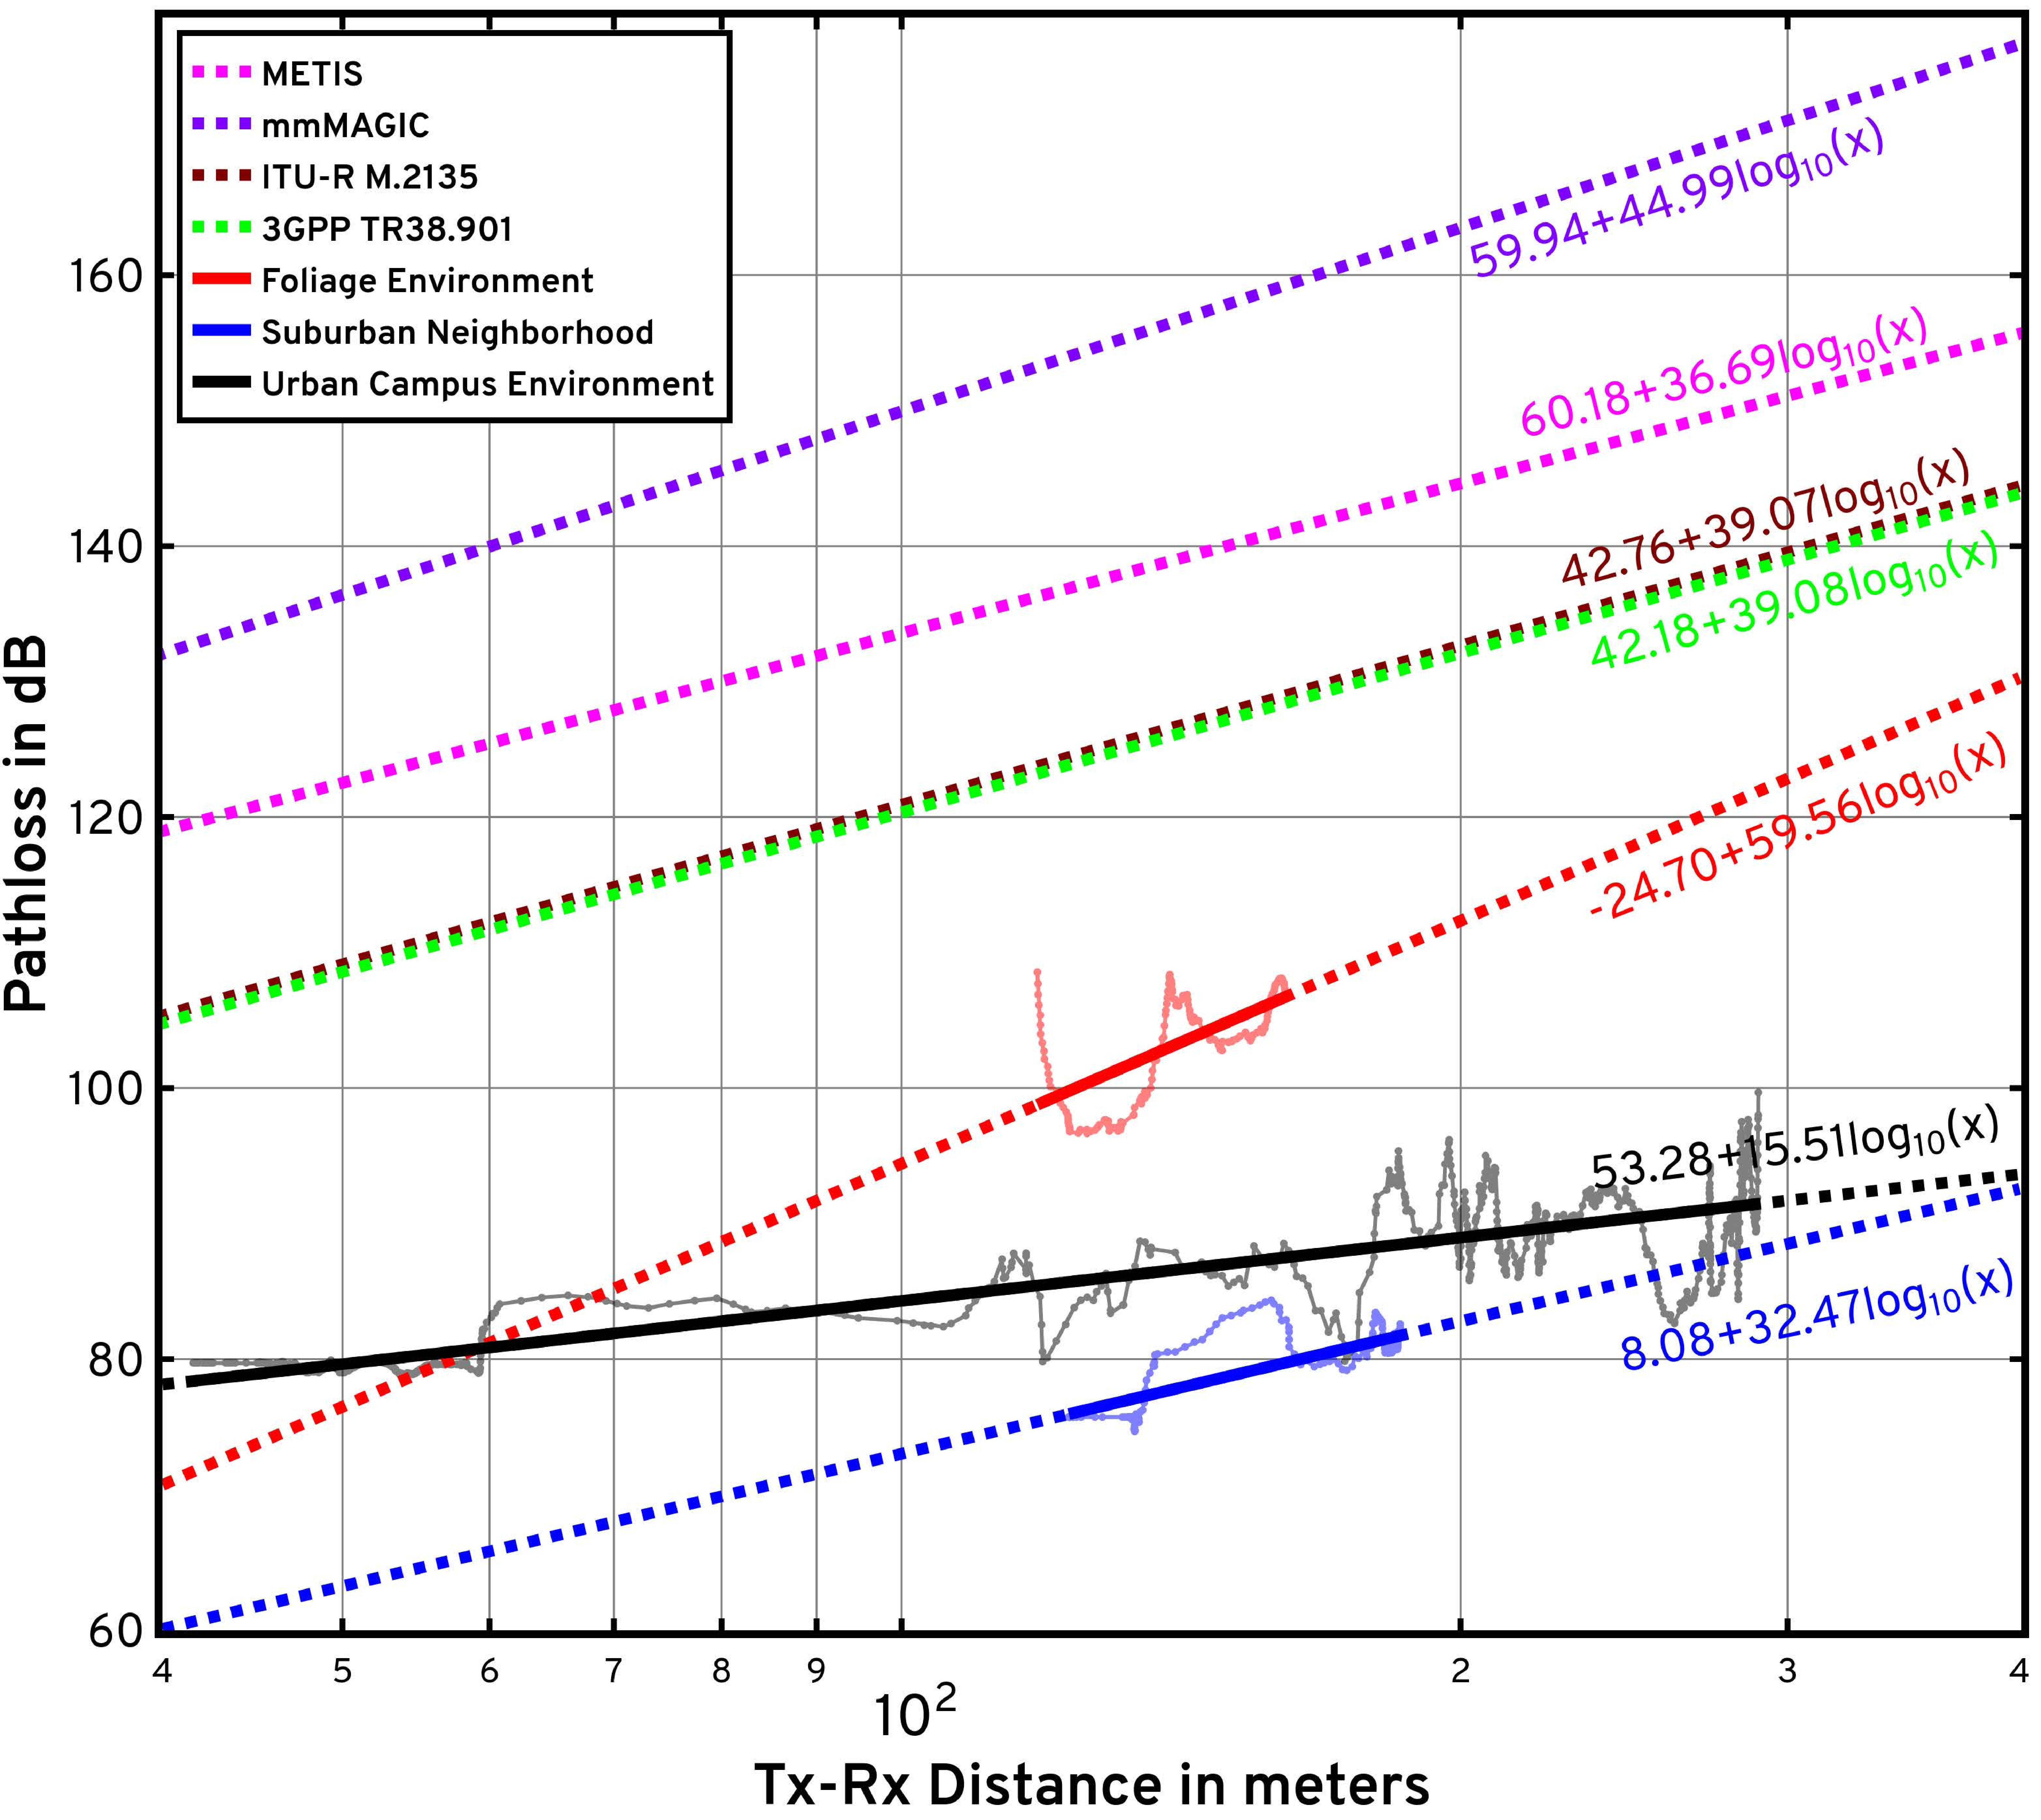
\includegraphics[width=1.0\linewidth]{figs/pathloss_vs_distance.pdf}
         \caption{Pathloss vs Tx-Rx Distance}
         \label{F7a}
     \end{subfigure}
     \begin{subfigure}{0.5065\linewidth}
         \centering
         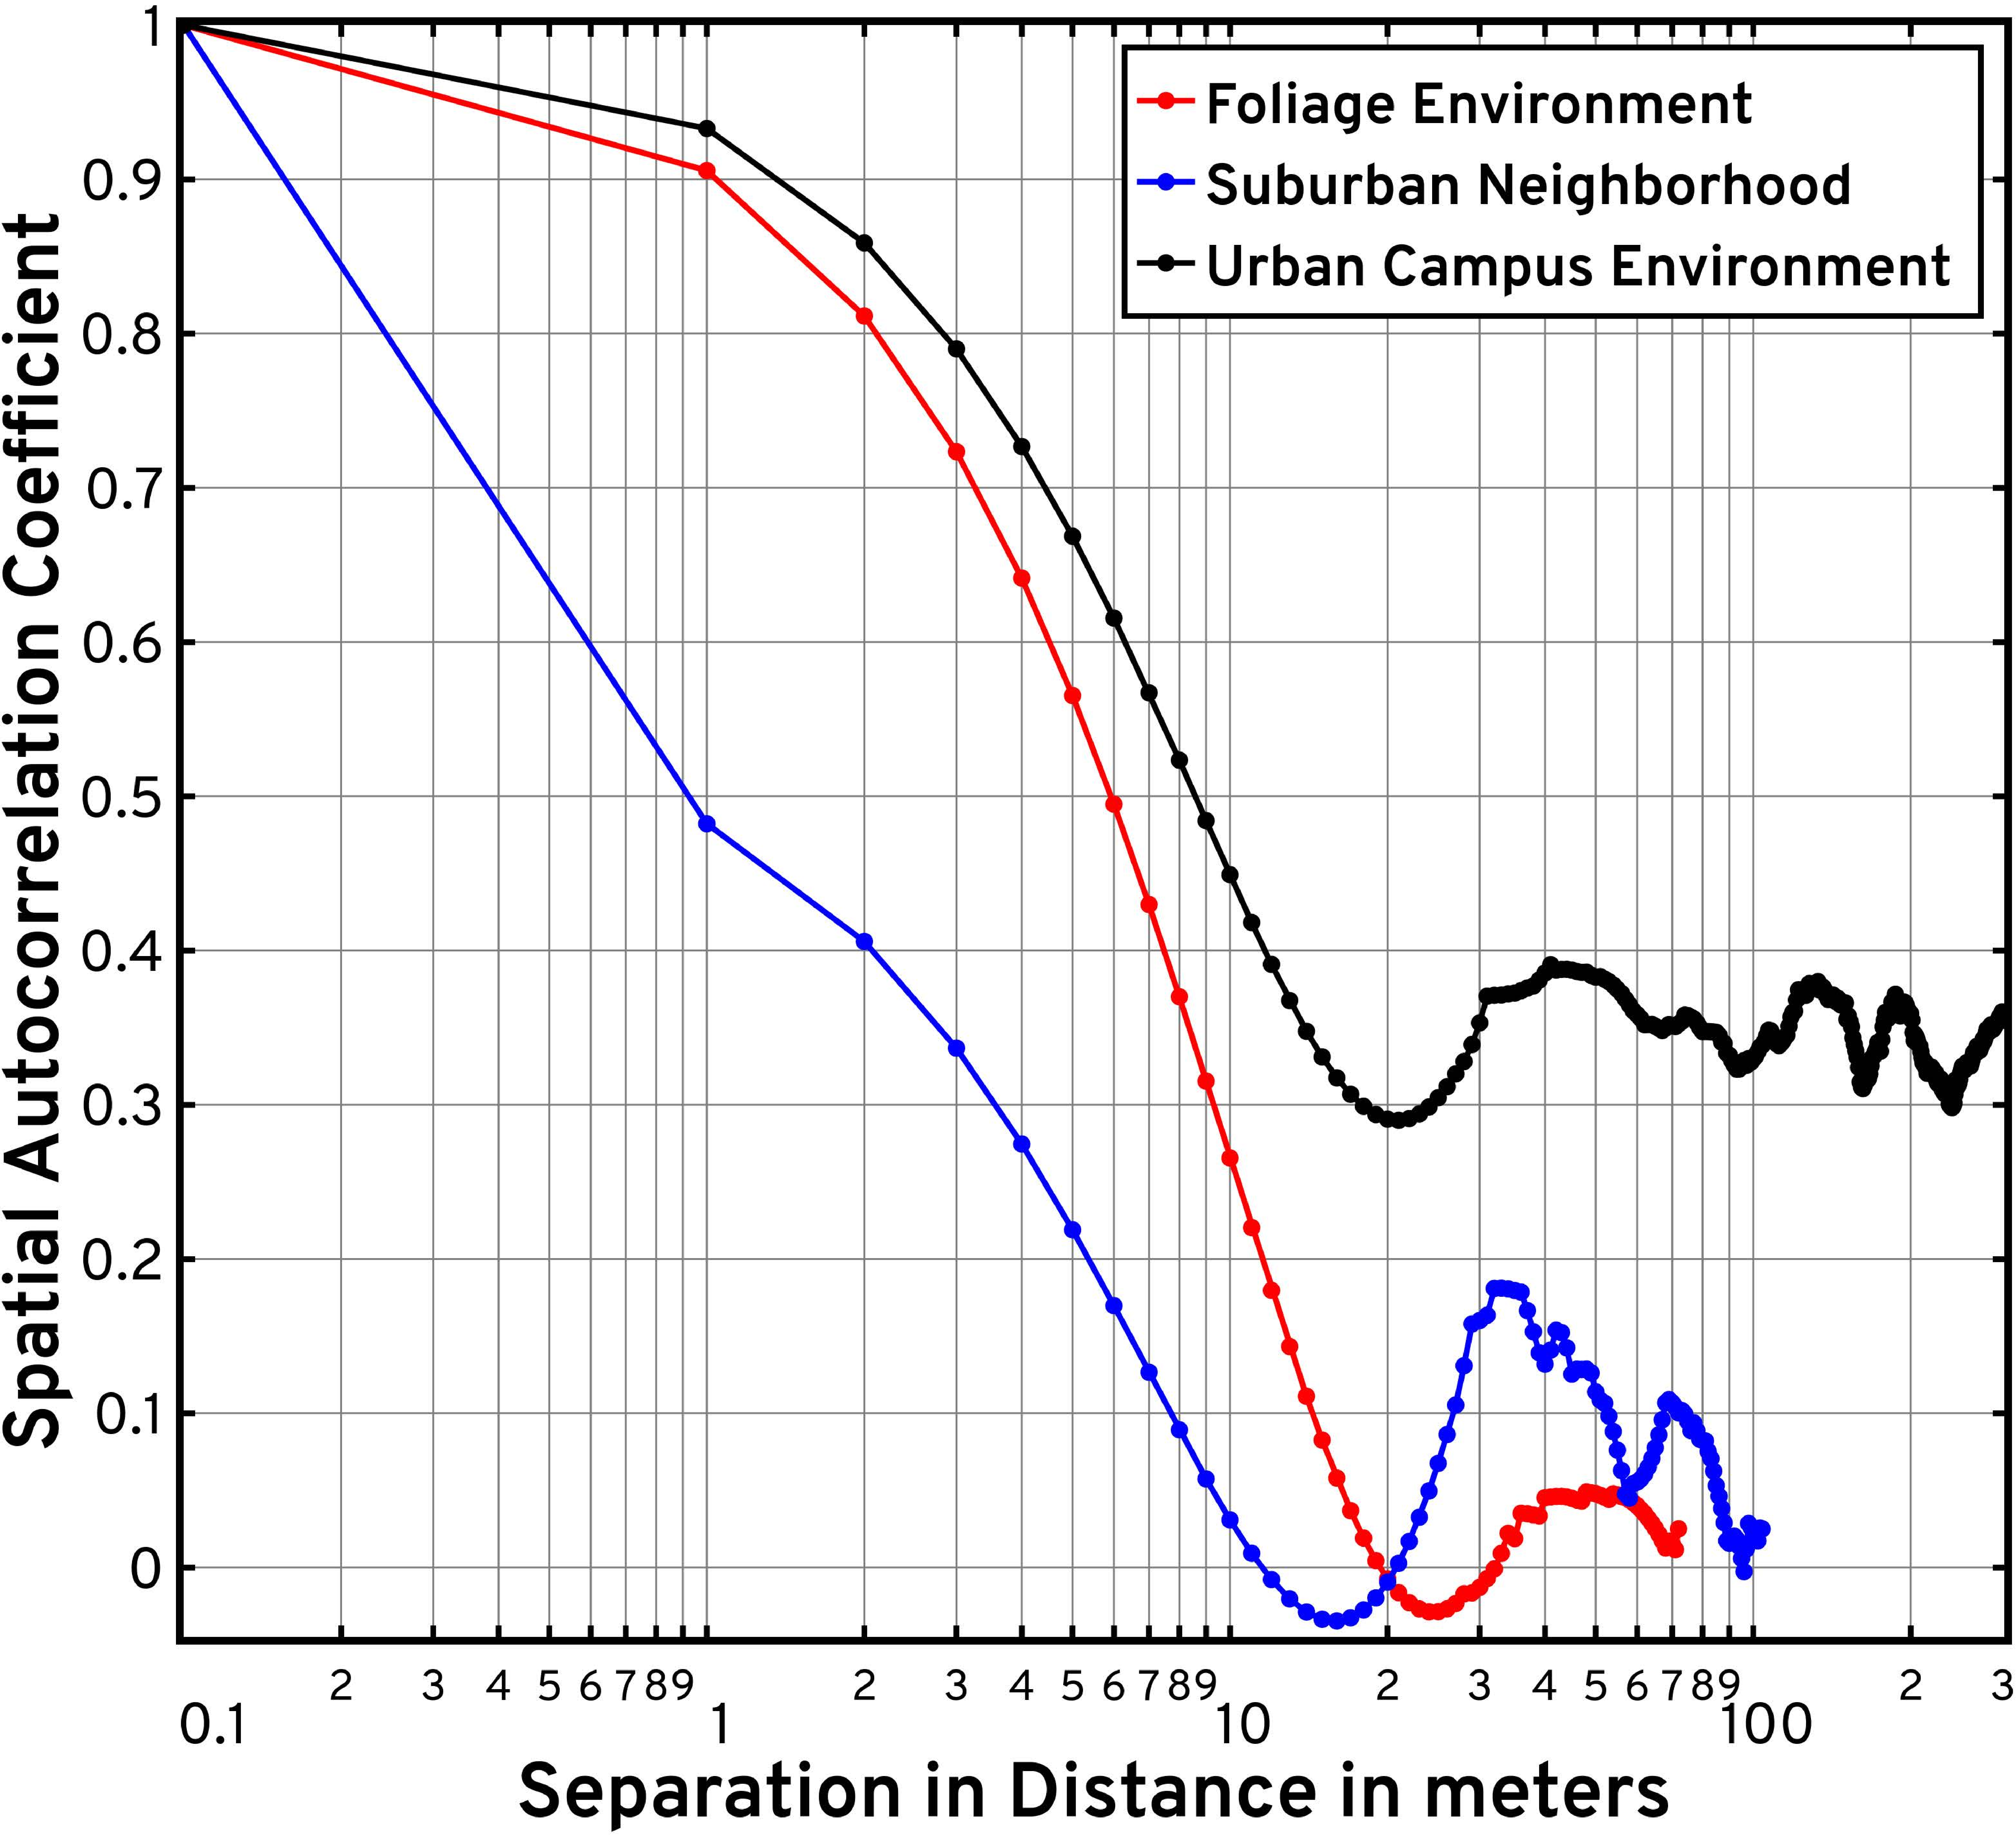
\includegraphics[width=1.0\linewidth]{figs/spatial_consistency_vs_distance.pdf}
         \caption{Spatial Consistency vs Distance}
         \label{F7b}
     \end{subfigure}
     \vspace{-8mm}
     \caption{An illustration of the measured and extrapolated pathloss vs log-distance behavior of mmWave signals in V$2$X settings, and their comparisons against the $3$GPP TR$38.901$, ITU-R M.$2135$, METIS, and mmMAGIC standards -- with the solid lines denoting our measurements and the dashed lines denoting the corresponding fitted models (a); and a plot depicting the variations in the spatial autocorrelation coefficient under separations in distance (b), i.e., $\rho(\Delta d)$ vs log-distance.}
     \label{F7}
\end{figure*}

\noindent{\textbf{Spatial Consistency}}: Finally, in this section, to study the spatial decoherence behavior of \SI{28}{\giga\hertz} signals in V$2$X scenarios, we evaluate the spatial autocorrelation coefficient along specific Rx routes under the effects of Tx-Rx distance, alignment accuracy, and relative velocity. Herein, we first describe the mathematical modeling underlying the computation of the spatial autocorrelation coefficient, after which we outline the insights gained from our results on the decorrelation characteristics of \SI{28}{\giga\hertz} signals in V$2$X settings under distance, alignment, and velocity effects.

The small-scale spatial autocorrelation coefficient is a metric to characterize the coherence between the voltage amplitudes of received signals across variations in distances, alignment accuracies, and relative velocities. With $\mathcal{I} \triangleq \{1,2,{\dots},I\}$ as the index set, we define a route in our measurement campaign as a set of $5$-tuples, i.e., $\mathcal{R} \triangleq \{\mathcal{T}_{i} \triangleq \left(\mathbf{x}_{i}, \mathbf{y}_{i}, \phi_{i}, v_{i}, \mathcal{M}_{i}\right) \suchthat i \in \mathcal{I}\}$, where $\mathbf{x}_{i}$ denotes the $3$D position vector of the Rx, $\mathbf{y}_{i}$ denotes the $3$D position vector of the Tx, $\phi_{i}$ denotes the accuracy of alignment between the Tx and Rx horn antennas (i.e., deviation from perfect alignment), and $v_{i}$ denotes the relative velocity of the Rx with respect to the Tx. Let $\mathcal{J}_{i} \triangleq \{1,2,{\dots},J_{i}\}$ represent the index set for the collection of measurements obtained at the route configuration index $i \in \mathcal{I}$; therefore, the corresponding set of measurements is defined as $\mathcal{M}_{i} \triangleq \{\mathbf{m}_{i,j} \suchthat j \in \mathcal{J}_{i}\}$. As detailed in Sec.~\ref{S3}, each vector of received samples $\mathbf{m}_{i,j}$ undergoes processing via pre-filtering, time-windowing, and noise elimination; subsequently, as mentioned earlier in this section, with propagation delay bins $\boldsymbol{\tau} \triangleq \{\tau_{1},\tau_{2},{\dots},\tau_{L}\}$ (e.g., $1$ ns to $1000$ ns quantization), we extract the amplitudes of the Multi-Path Components (MPCs) at these delay bins using the SAGE algorithm~\cite{SAGE}, i.e., $\forall i \in \mathcal{I}$, we define the corresponding local set of MPC amplitudes across all delay bins as $\tilde{\mathcal{M}}_{i} \triangleq \left\{\Big[A_{i,j}(\tau_{1}), A_{i,j}(\tau_{2}), \dots, A_{i,j}(\tau_{L})\Big]^{\mathsf{T}} \suchthat j \in \mathcal{J}_{i}\right\}$.

With the Tx fixed ($\mathbf{y}_{i} = \mathbf{y}, \forall i \in \mathcal{I}$), we define the following evaluation conditions to compute the spatial autocorrelation coefficient~\cite{MacCartneySpatialStatistics} under variations in three separation variables, viz., separation in distance $\Delta d$, Tx-Rx alignment accuracy $\Delta \phi$, and Tx-Rx relative velocity $\Delta v$:\clearpage
\begin{align}\label{Ed}
    \mathcal{I}(\Delta d) \triangleq \left\{(i,i') \in \binom{\mathcal{I}}{2}: \norm{\mathbf{x}_{i} - \mathbf{x}_{i'}} = \Delta d, \phi_{i} = \phi_{i'}, v_{i} = v_{i'}\right\};
\end{align}
\begin{align}\label{Ea}
    \mathcal{I}(\Delta \phi) \triangleq \left\{(i,i') \in \binom{\mathcal{I}}{2}: \mathbf{x}_{i} = \mathbf{x}_{i'}, \abs{\phi_{i} - \phi_{i'}} = \Delta \phi, v_{i} = v_{i'}\right\};
\end{align}
\begin{align}\label{Ev}
    \mathcal{I}(\Delta v) \triangleq \left\{(i,i') \in \binom{\mathcal{I}}{2}: \mathbf{x}_{i} = \mathbf{x}_{i'}, \phi_{i} = \phi_{i'}, \abs{v_{i} - v_{i'}} = \Delta v\right\}.
\end{align}
For the MPC at delay bin $\tau_{l} \in \boldsymbol{\tau}$, the local amplitude mean (temporal average) across the set of measurements collected at a route configuration index $i \in \mathcal{I}$ is $A_{i}(\tau_{l}) \triangleq \frac{1}{J_{i}}\sum_{j = 1}^{J_{i}}\ A_{i,j}(\tau_{l})$. Let $\mathbf{d} \triangleq \{d_{1},d_{2},{\dots},d_{K}\}$ be the Tx-Rx distance bins (quantization of distances) along this route $\mathcal{R}$ indexed by the set $\mathcal{I}$; similarly, let $\boldsymbol{\phi} \triangleq \{\phi_{1},\phi_{2},{\dots},\phi_{M}\}$ denote the Tx-Rx alignment accuracy bins and let $\mathbf{v} \triangleq \{v_{1},v_{2},{\dots},v_{N}\}$ denote the Tx-Rx relative velocity bins. Then, we define $\mathcal{I}(d_{k}, \phi_{m}, v_{n}) \triangleq \{i \in \mathcal{I}: \norm{\mathbf{x}_{i} - \mathbf{y}_{i}} \approx d_{k}, \phi_{i} \approx \phi_{m}, v_{i} \approx v_{n}\}$ as the set of route configuration indices for which their Tx-Rx distance belongs to distance bin $d_{k}$, their Tx-Rx alignment accuracy belongs to alignment bin $\phi_{m}$, and their Tx-Rx relative velocity belongs to velocity bin $v_{n}$ (note that in this definition the binning-based quantization is represented with the $\approx$ notation). Thus, using these definitions and the evaluation condition described by the index set in Eq.~\eqref{Ed}, we compute the spatial autocorrelation coefficient $\rho$ vis-à-vis a separation in distance $\Delta d$ as 
\begin{align}\label{SCD}
    \rho(\Delta d) = \frac{\frac{1}{|\mathcal{I}(\Delta d)|}\sum_{(i,i') \in \mathcal{I}(\Delta d)}\Bigg[\sum_{l = 1}^{L}\bigg(\Big(A_{i}(\tau_{l}) - \mu_{i}(\tau_{l})\Big)\Big(A_{i'}(\tau_{l}) - \mu_{i'}(\tau_{l})\Big)\bigg)\Bigg]}{\frac{1}{|\mathcal{I}|}\sum_{i \in \mathcal{I}}\bigg[\sum_{l = 1}^{L}\Big(A_{i}(\tau_{l}) - \mu_{i}(\tau_{l})\Big)^{2}\bigg]},
\end{align}
where for a route configuration index $i \in \mathcal{I}$ with its Tx-Rx distance in distance bin $d_{k} \in \mathbf{d}$, Tx-Rx alignment accuracy in alignment bin $\phi_{m} \in \boldsymbol{\phi}$, and Tx-Rx relative velocity in velocity bin $v_{n} \in \mathbf{v}$, the amplitude sample mean (spatial average) of the MPC at delay bin $\tau_{l} \in \boldsymbol{\tau}$ is defined as $\mu_{i}(\tau_{l}) = \frac{1}{|\mathcal{I}(d_{k}, \phi_{m}, v_{n})|}\sum_{\iota = 1}^{|\mathcal{I}(d_{k}, \phi_{m}, v_{n})|}\ A_{\iota}(\tau_{l})$; and similarly, for a route configuration index $i' \in \mathcal{I}$ with its Tx-Rx distance in distance bin $d_{k'} \in \mathbf{d}$, Tx-Rx alignment accuracy in alignment bin $\phi_{m} \in \boldsymbol{\phi}$, and Tx-Rx relative velocity in velocity bin $v_{n} \in \mathbf{v}$, the amplitude sample mean (spatial average) of the MPC at delay bin $\tau_{l} \in \boldsymbol{\tau}$ is defined as $\mu_{i'}(\tau_{l}) = \frac{1}{|\mathcal{I}(d_{k'}, \phi_{m}, v_{n})|}\sum_{\iota = 1}^{|\mathcal{I}(d_{k'}, \phi_{m}, v_{n})|}\ A_{\iota}(\tau_{l})$. Note that the sets used to compute these amplitude sample means for $i, i' \in \mathcal{I}$ could potentially differ only in their Tx-Rx distance bin, i.e., consistent with the condition~\eqref{Ed}, they belong to the same alignment and velocity bins. In a similar vein, we compute the spatial autocorrelation coefficients under variations in the alignment and velocity separation variables, i.e., $\rho(\Delta \phi)$ and $\rho(\Delta v)$, respectively. Specifically, the index set representing the evaluation condition in Eq.~\ref{SCD} is replaced with $\mathcal{I}(\Delta \phi)$ for $\rho(\Delta \phi)$ and with $\mathcal{I}(\Delta v)$ for $\rho(\Delta v)$; also, the amplitude sample means $\mu_{i}(\tau_{l})$ and $\mu_{i'}(\tau_{l})$ involve index sets that could potentially differ only in their corresponding separation variables, i.e., alignment bins ($\phi_{m}$ and $\phi_{m'}$) or velocity bins ($v_{n}$ and $v_{n'}$), respectively.\\
\begin{figure*} [t]
     \centering
     \begin{subfigure}{0.5015\linewidth}
         \centering
         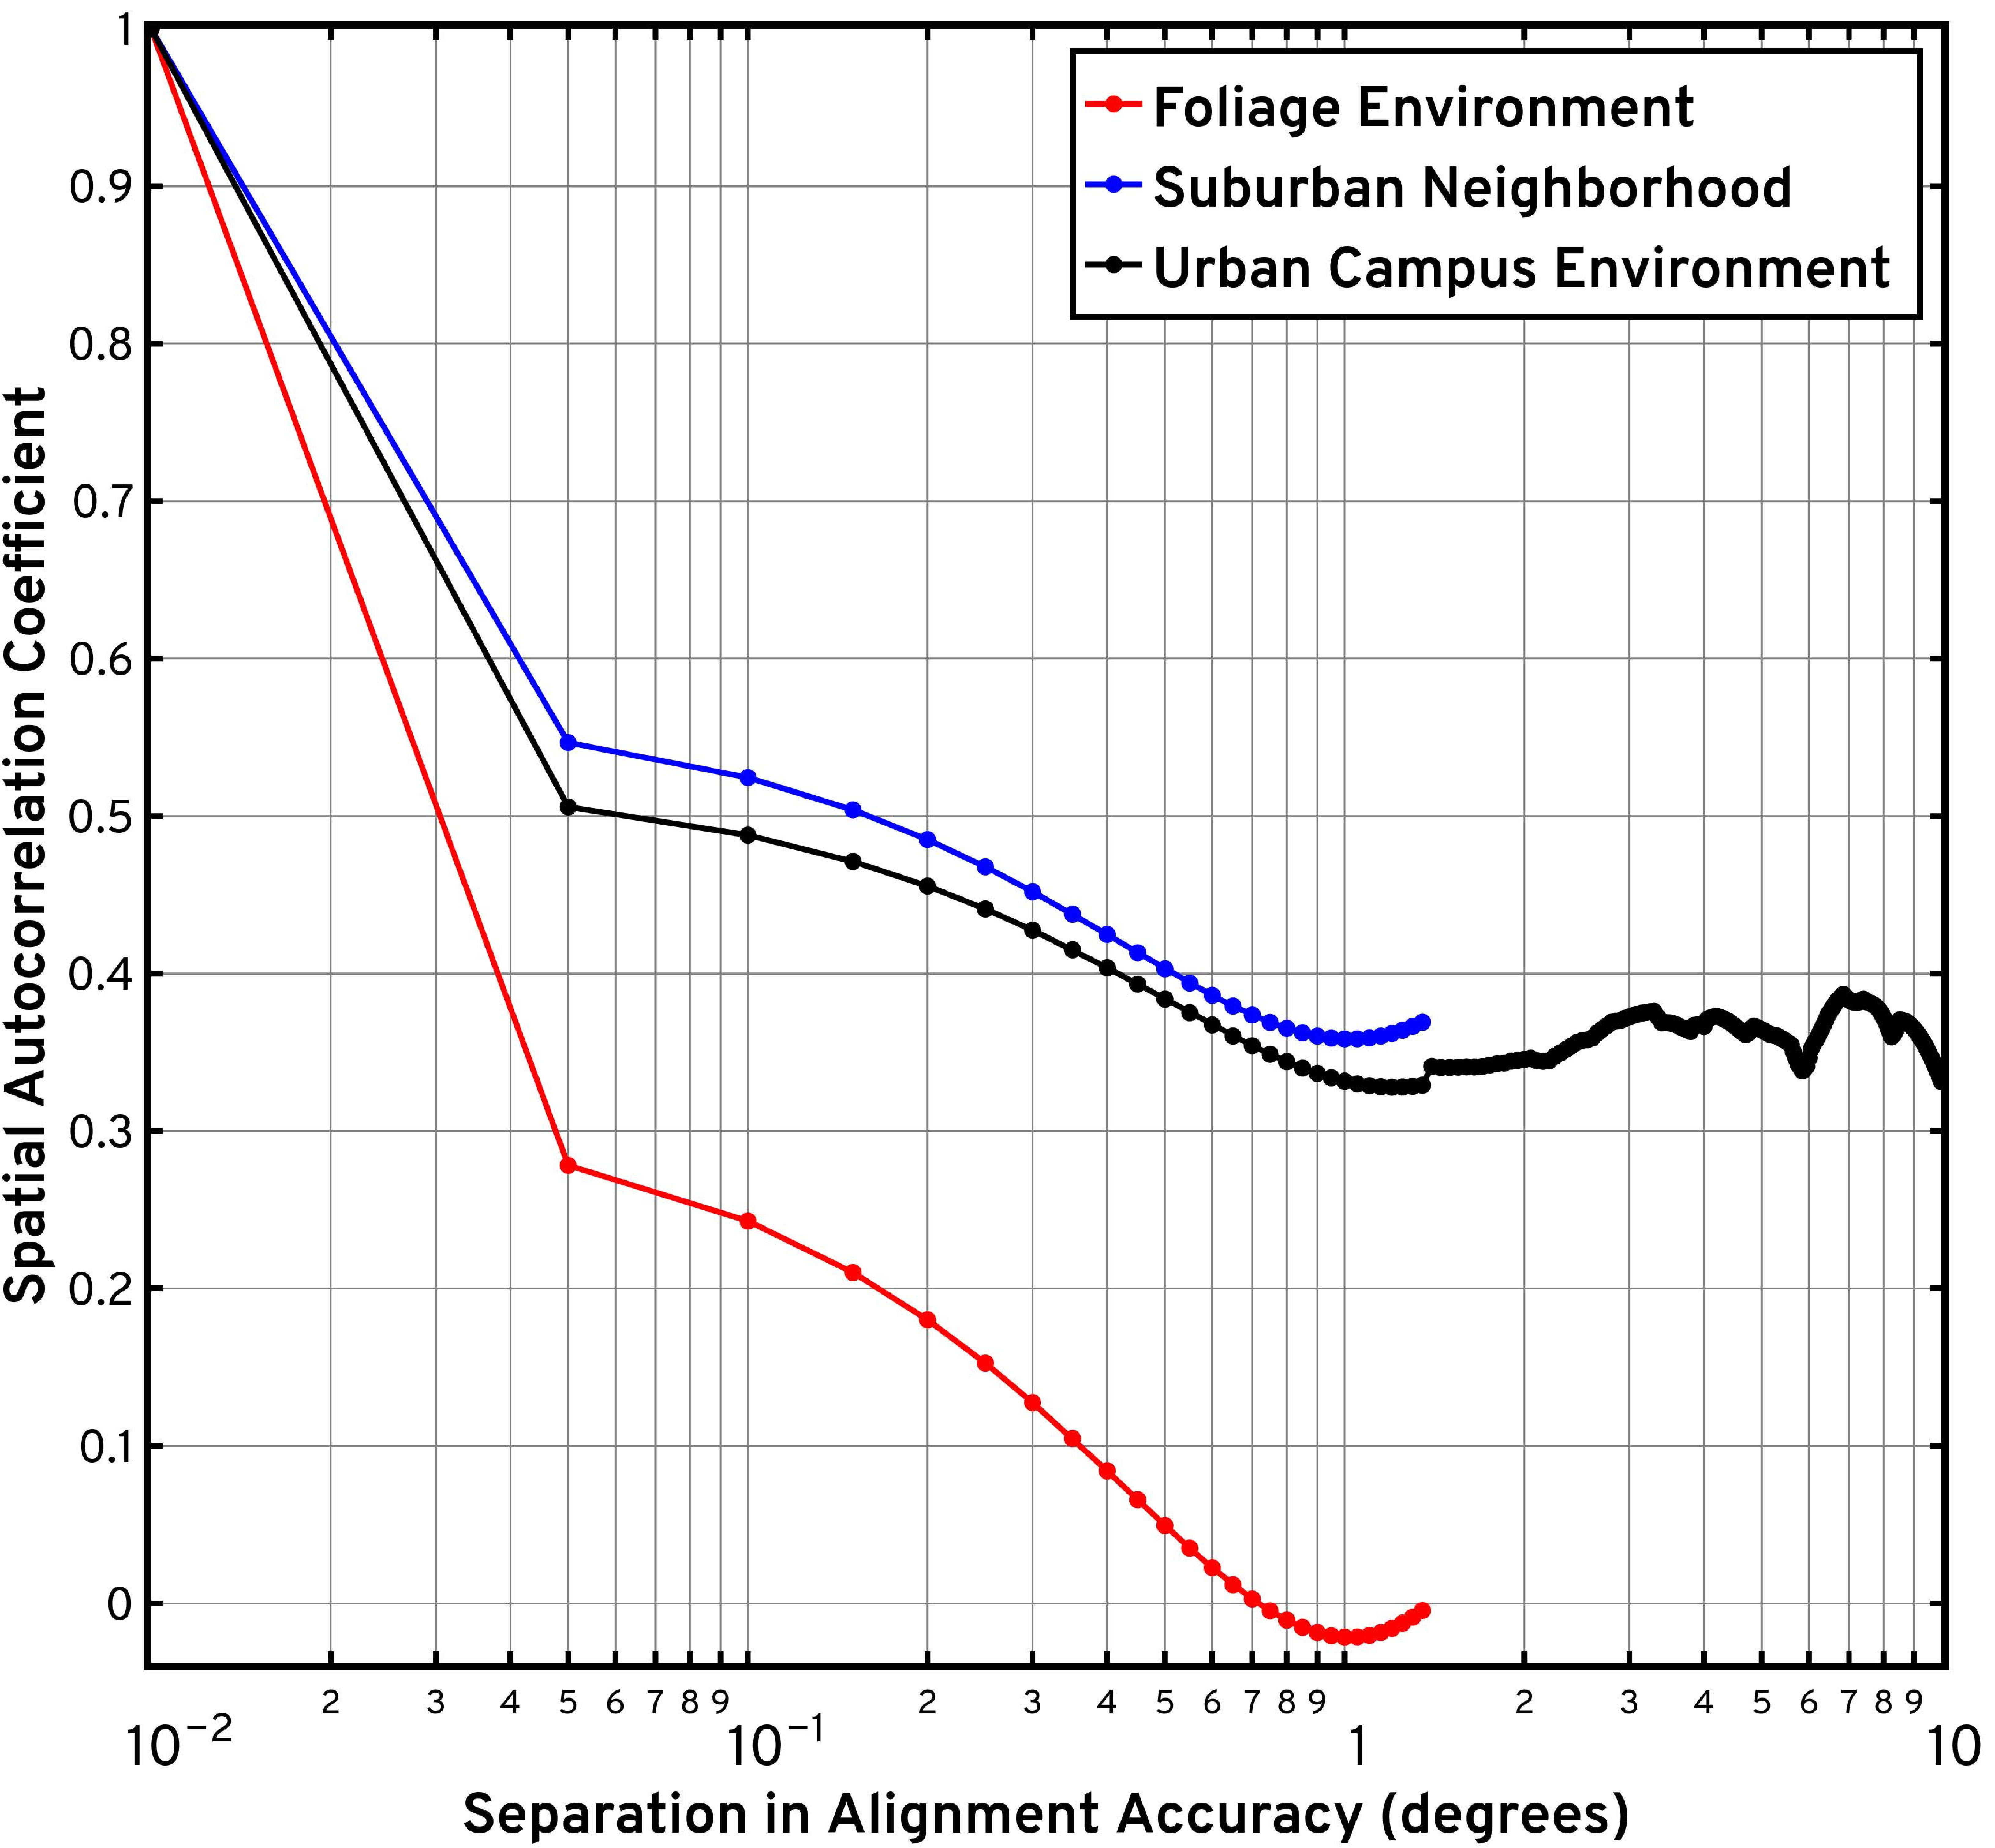
\includegraphics[width=1.0\linewidth]{figs/spatial_consistency_vs_alignment.pdf}
         \caption{Spatial Consistency vs Tx-Rx Alignment Accuracy}
         \label{F8a}
     \end{subfigure}
     \begin{subfigure}{0.4885\linewidth}
         \centering
         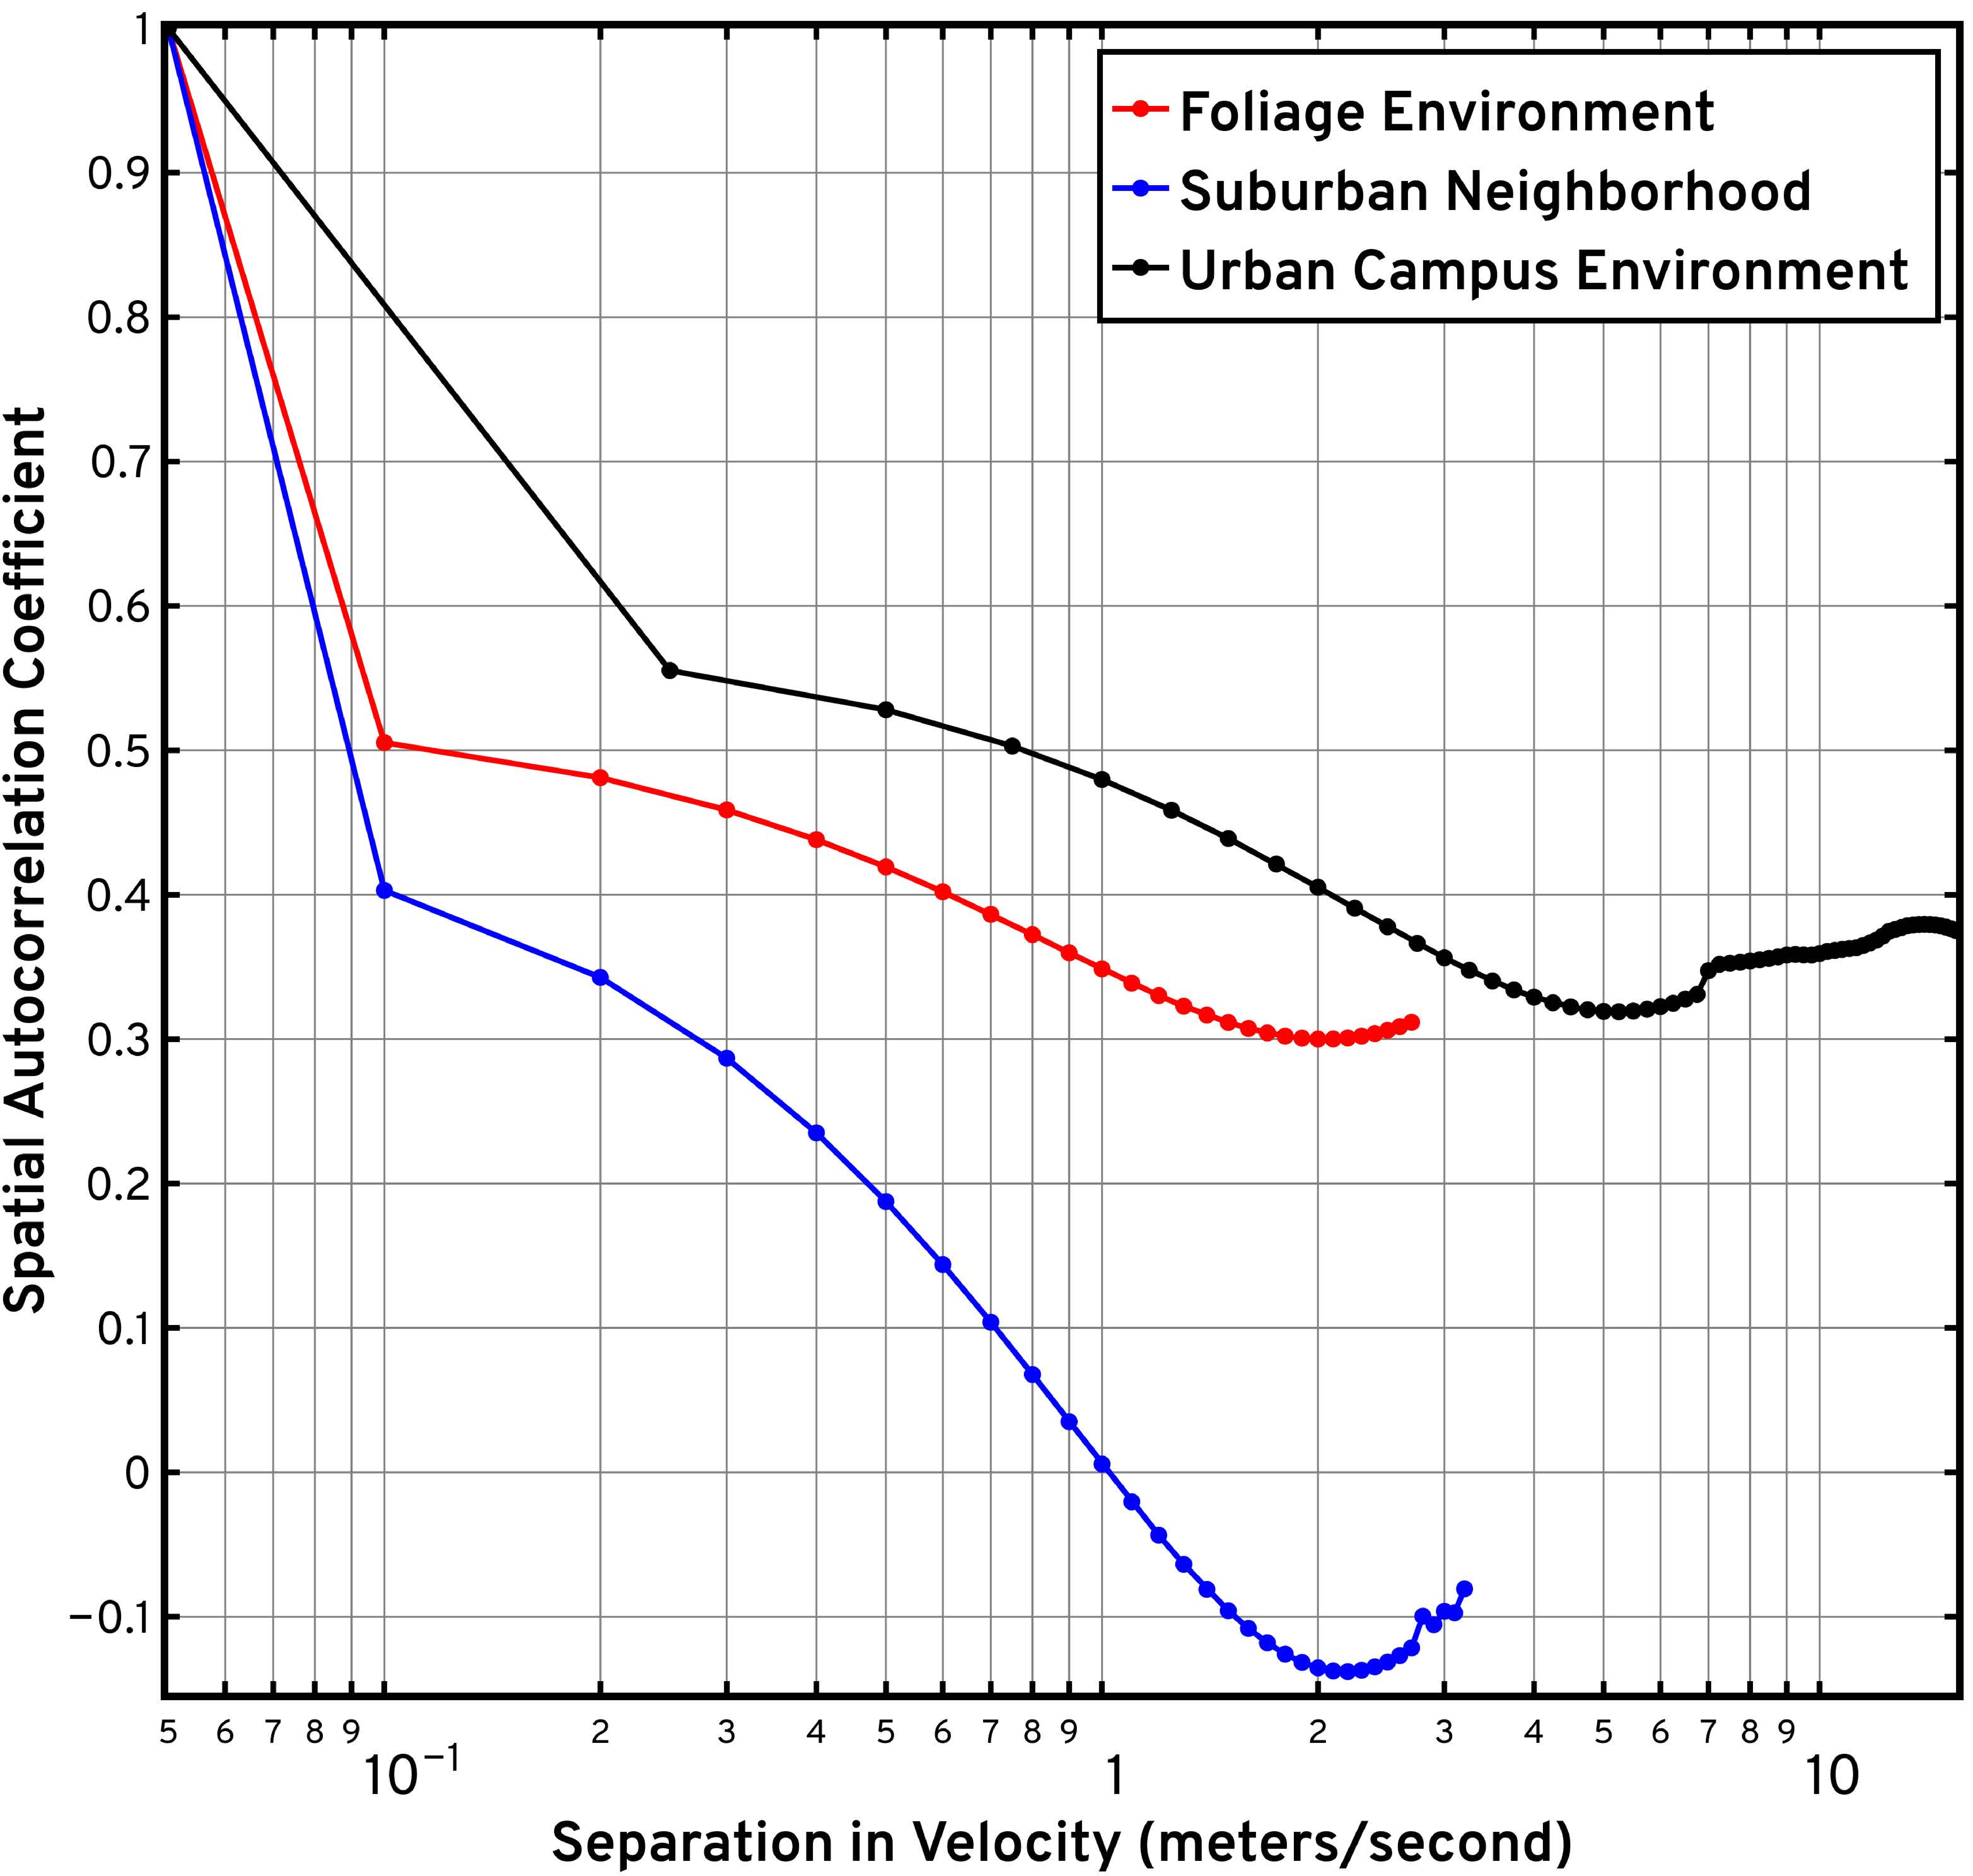
\includegraphics[width=1.0\linewidth]{figs/spatial_consistency_vs_velocity.pdf}
         \caption{Spatial Consistency vs Tx-Rx Relative Velocity}
         \label{F8b}
     \end{subfigure}
     \vspace{-8mm}
     \caption{The plots illustrating the behavior of the spatial autocorrelation coefficient under separations in Tx-Rx alignment accuracy and Tx-Rx relative velocity, i.e., $\rho(\Delta \phi)$ vs log-alignment (a) and $\rho(\Delta v)$ vs log-velocity (b).}
     \label{F8}
\end{figure*}
\indent{As} a result of the framework described above, Fig.~\ref{F7b} illustrates the spatial consistency curves as a function of the separations in distance for the urban campus, suburban neighborhood, and foliage environment routes. We note decreasing correlation trends between the recorded power delay profile samples under increasing distance separation. Similarly, Fig.~\ref{F8a} depicts the variation of the spatial autocorrelation coefficient under increasing levels of misalignment between the Tx and Rx antennas while traversing the urban campus, suburban neighborhood, and foliage environment routes. We observe rapid decorrelation across the evaluated samples even at small amounts of misalignment, highlighting the highly-directional characteristics of our WR-$28$ horn antennas, and illustrating the need for accurate beam-steering in mmWave V$2$X networks. Lastly, Fig.~\ref{F8b} depicts the spatial consistency characteristics of \SI{28}{\giga\hertz} signals under variations in the Tx-Rx relative velocity: here again, we observe considerably high levels of signal decoherence under small variations in the velocity of the Rx relative to the Tx, thereby further validating our claim about the need for a reliable and responsive beam-steering setup in mmWave systems for V$2$X applications. Note that, in Fig.~\ref{F7b}, Fig.~\ref{F8a}, and Fig.~\ref{F8b}, the channel does not get fully decorrelated since in our beam-steered setup, the LoS component always remains significant.
\begin{figure*} [t]
     \centering
     \begin{subfigure}{0.4815\linewidth}
         \centering
         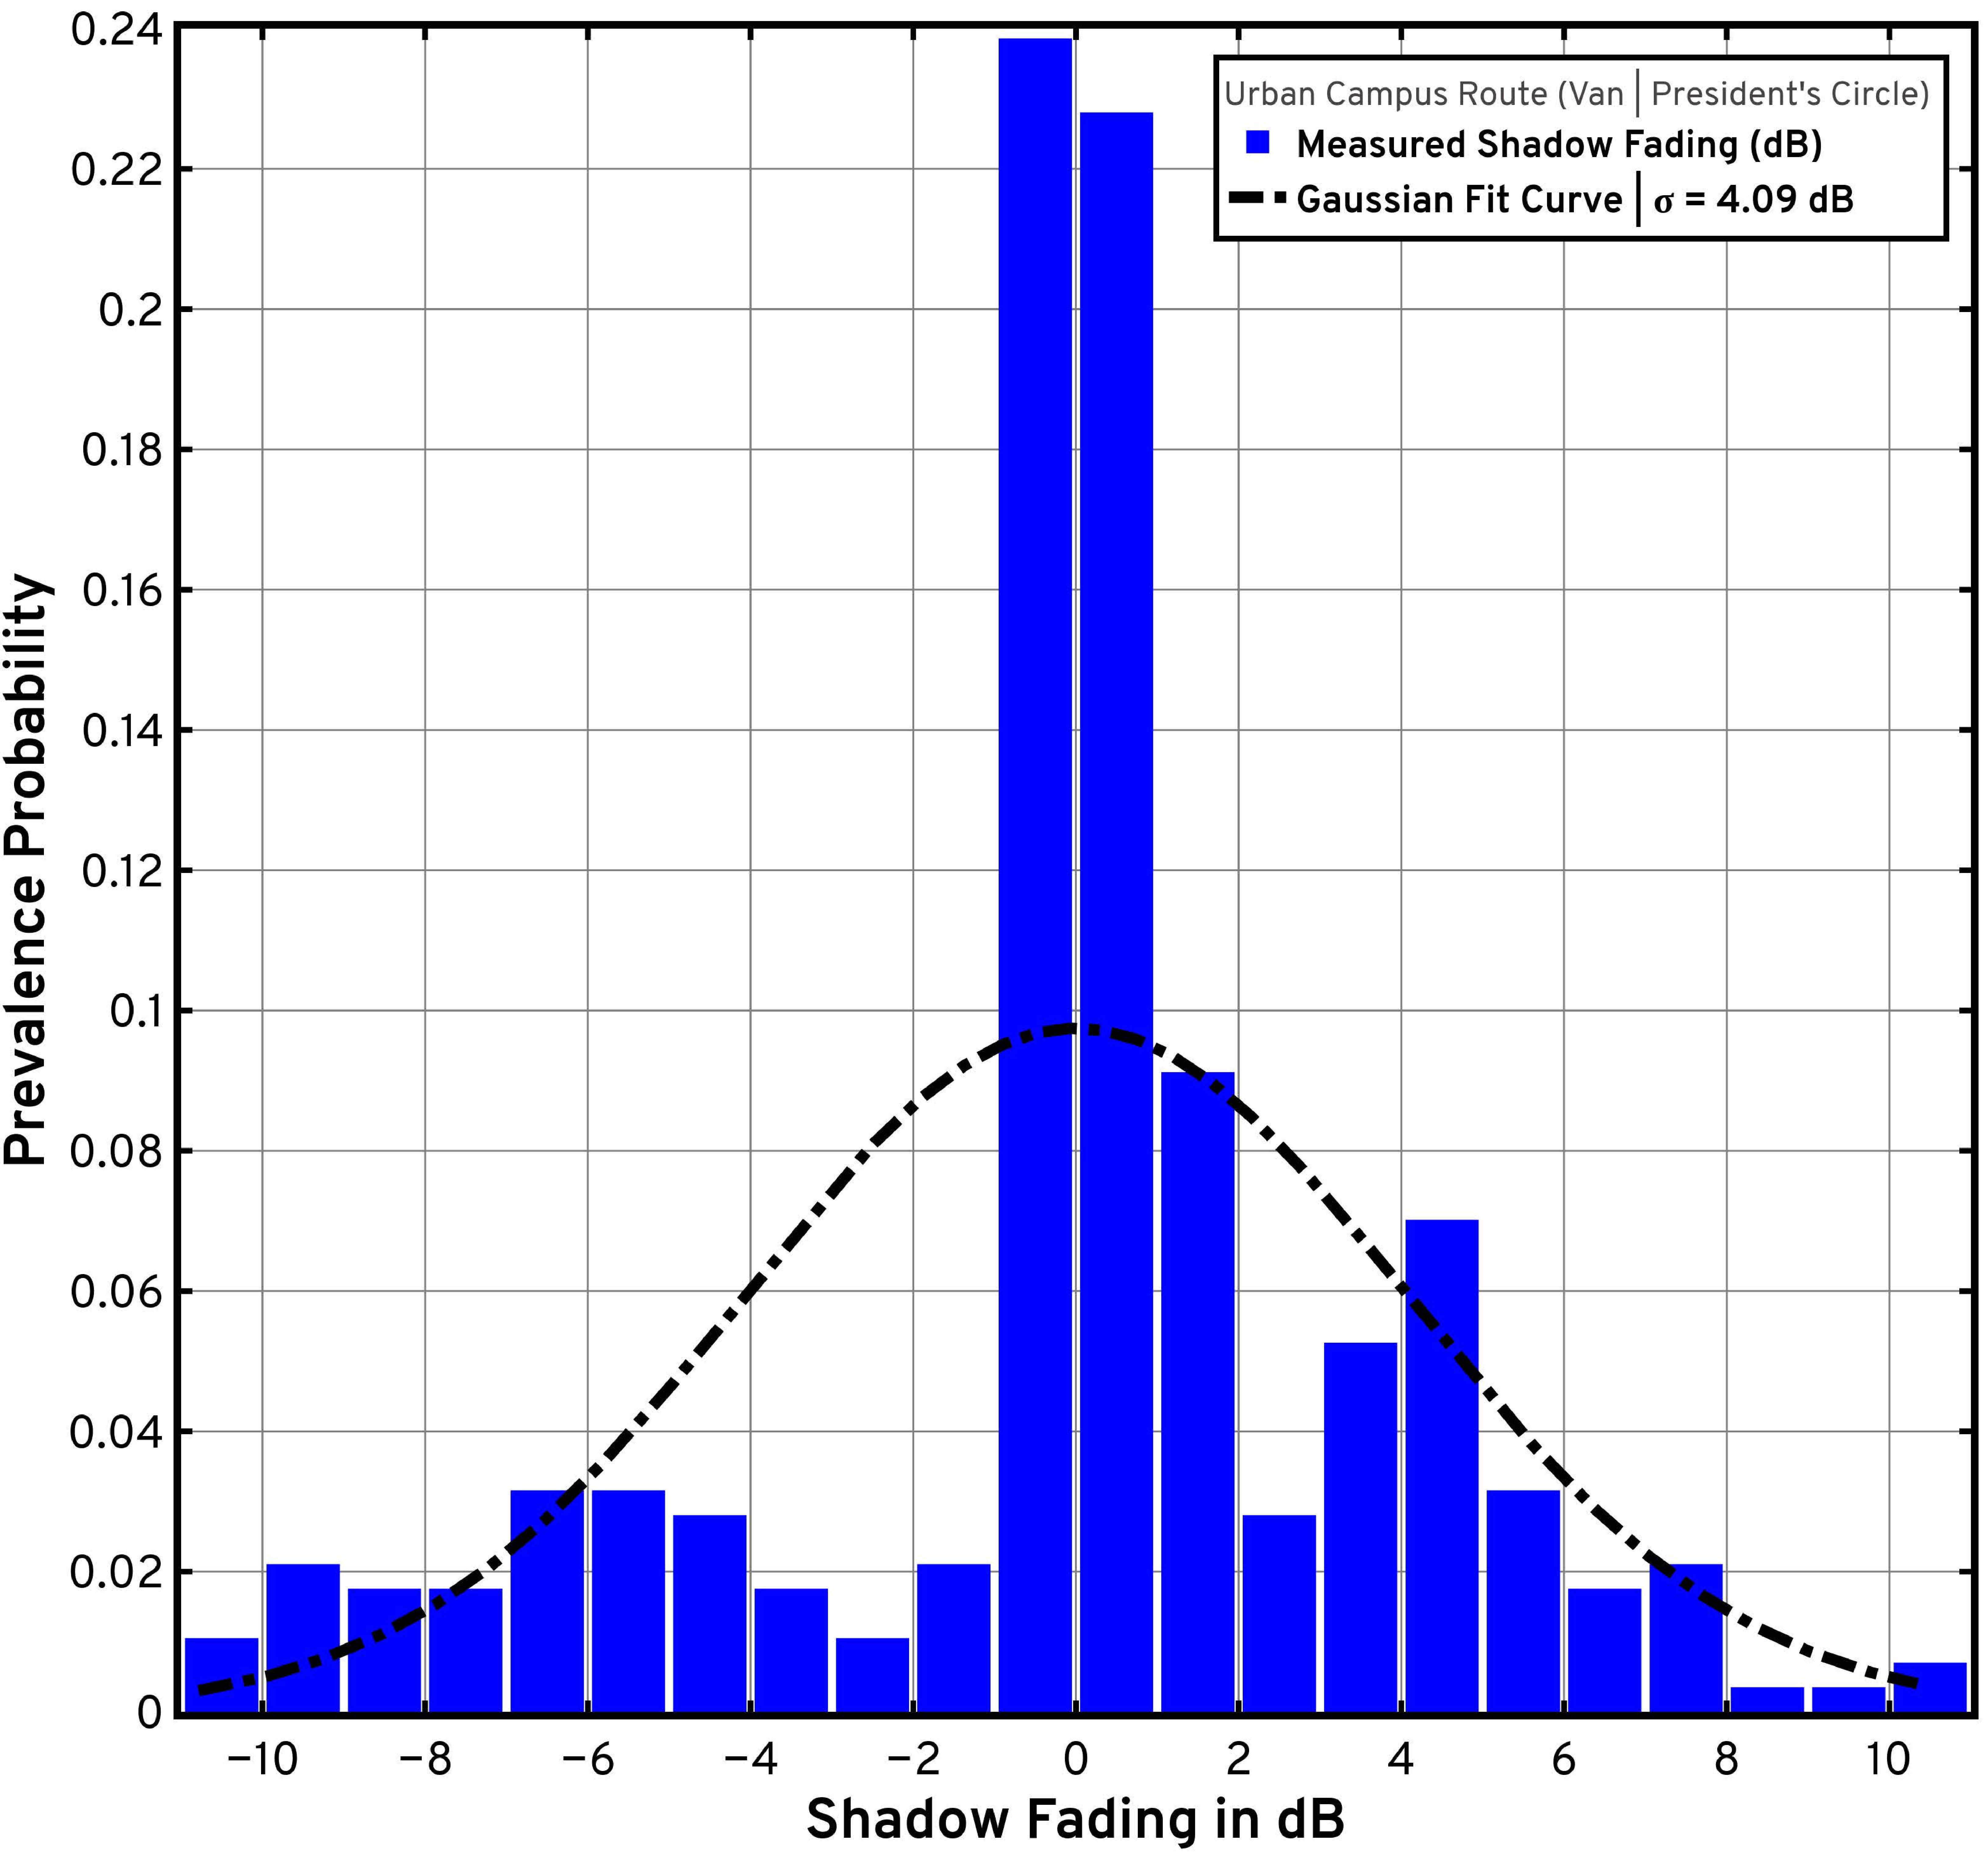
\includegraphics[width=1.0\linewidth]{figs/urban_campus_fading_1.pdf}
         \caption{Urban Campus (President's Circle)}
         \label{F9a}
     \end{subfigure}
     \begin{subfigure}{0.5085\linewidth}
         \centering
         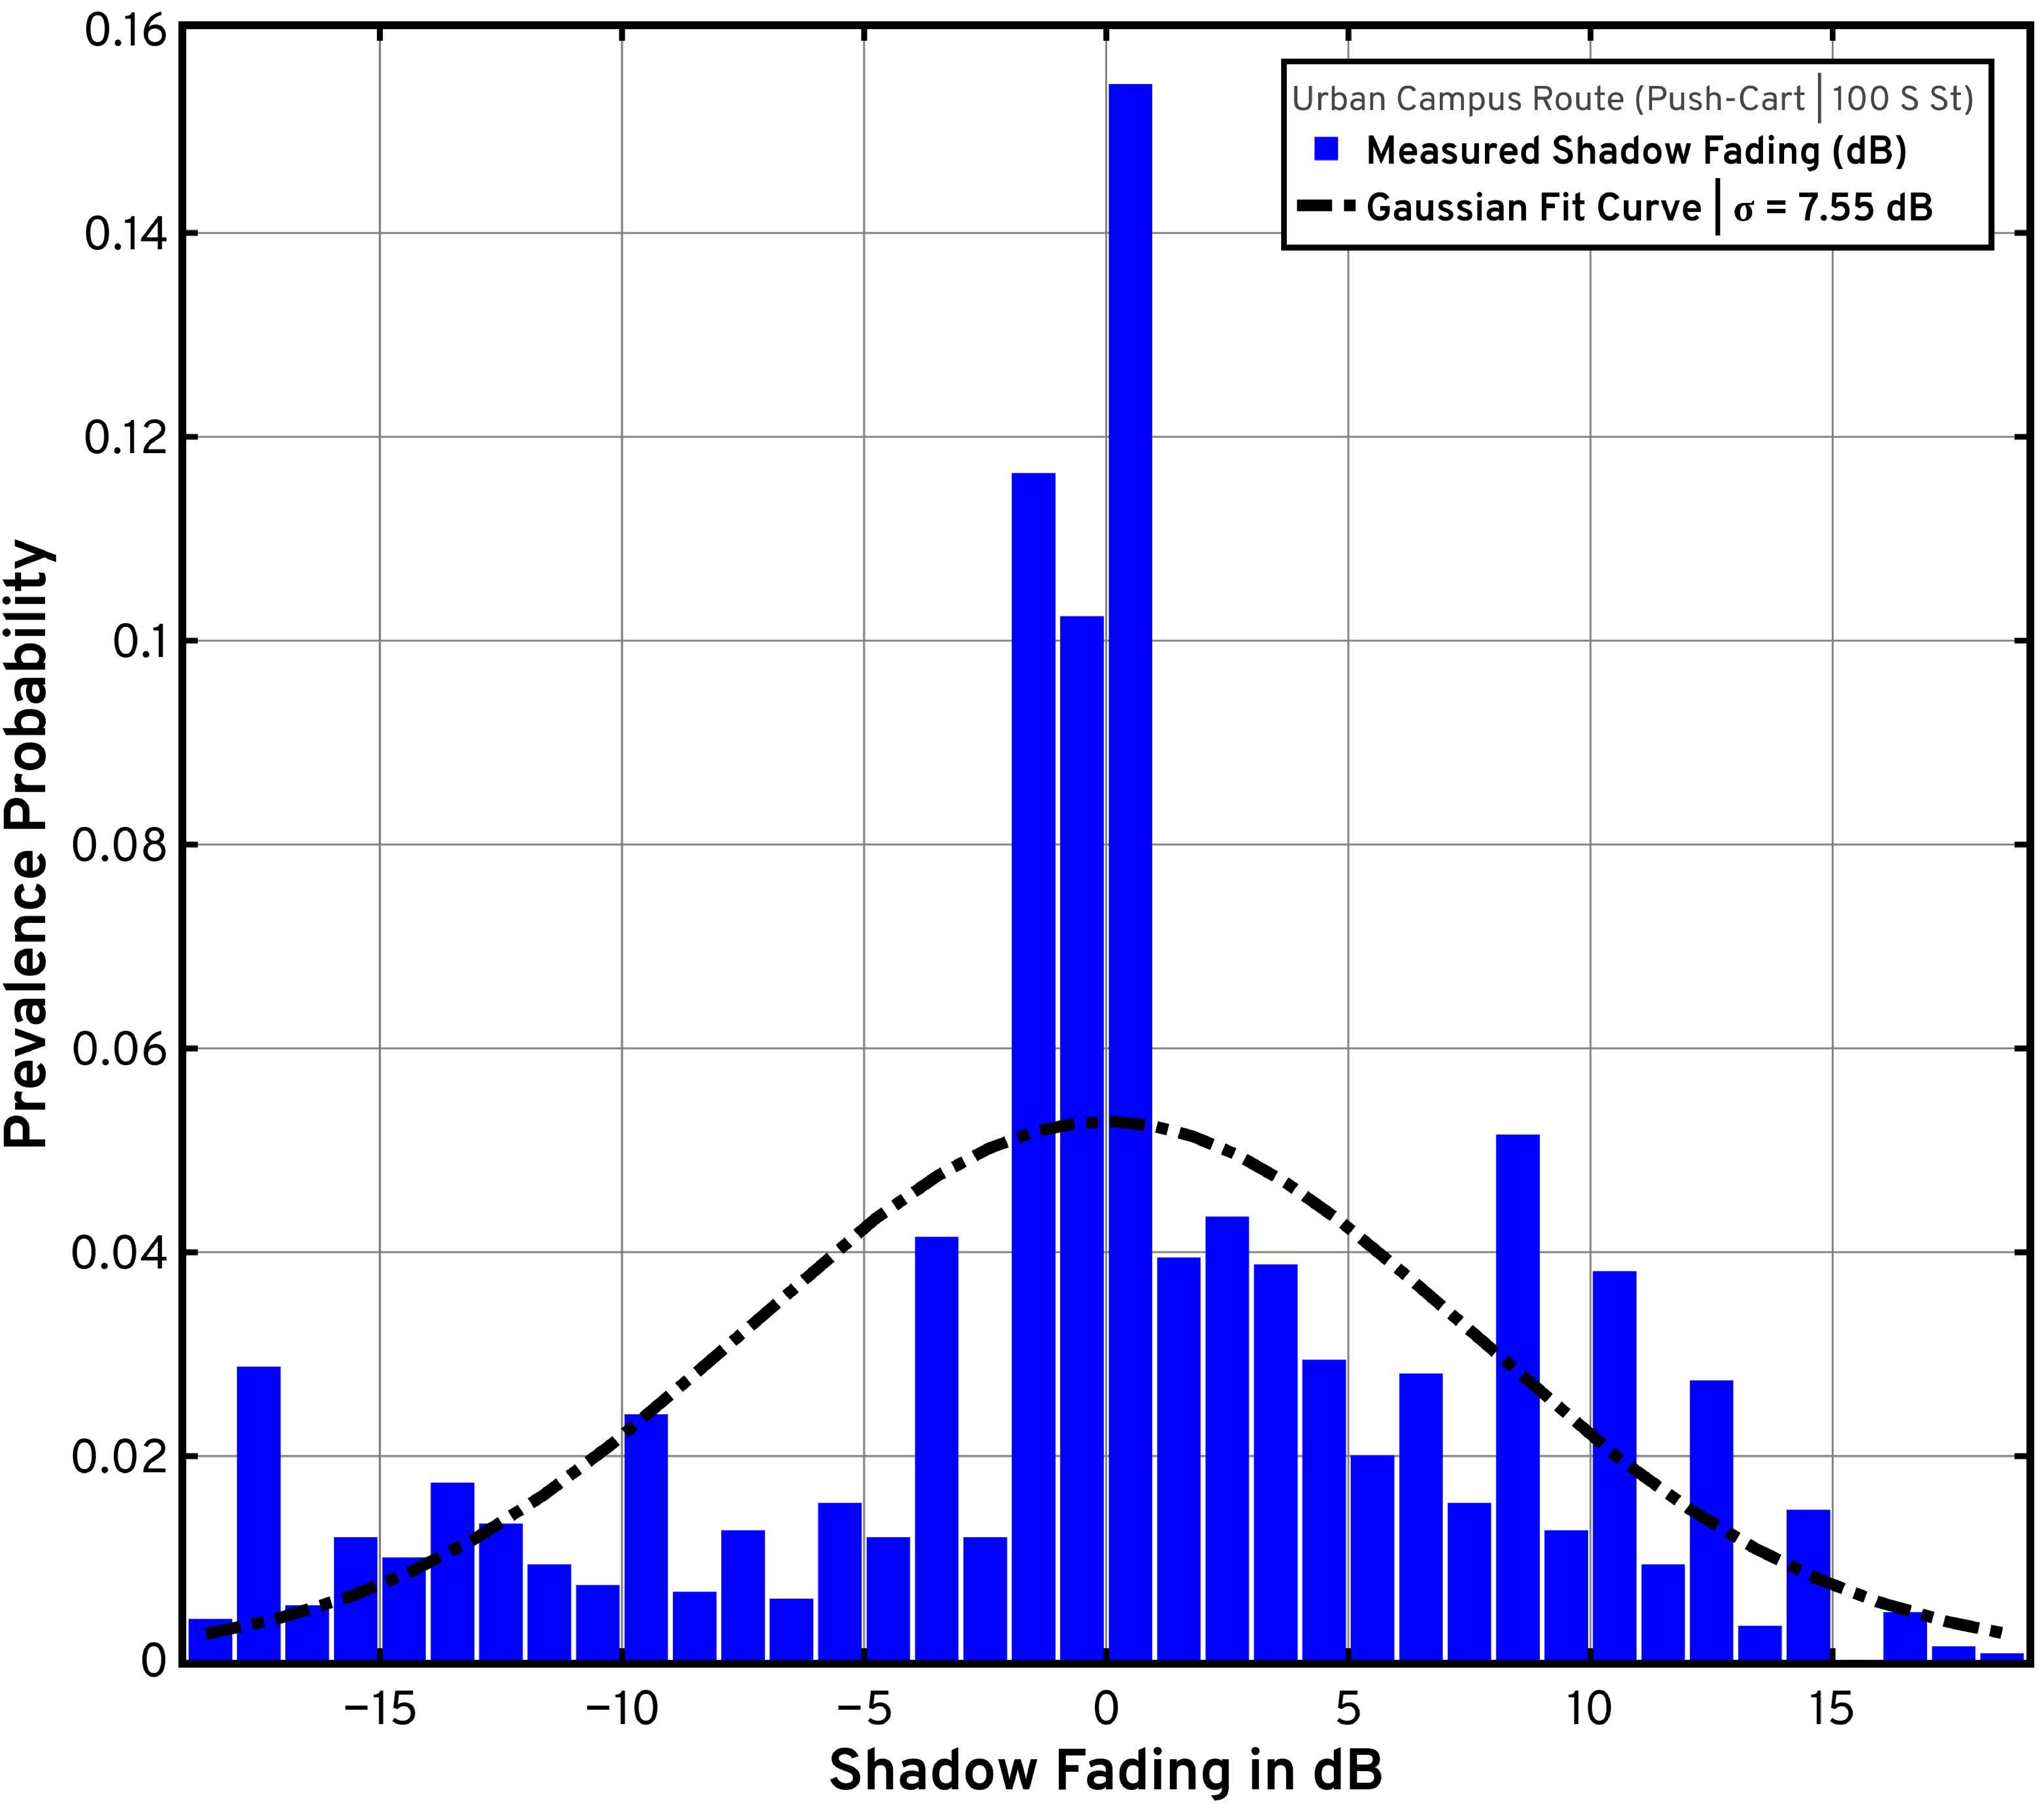
\includegraphics[width=1.0\linewidth]{figs/urban_campus_fading_2.pdf}
         \caption{Urban Campus (100 S St)}
         \label{F9b}
     \end{subfigure}
     \vspace{-8mm}
     \caption{The histograms and their corresponding Gaussian fits for the shadow fading effects experienced by mmWave signals along the urban campus routes onsite, viz., President's Circle (a) (Rx is on a minivan) and 100 S St (b) (Rx is on a push-cart).}
     \label{F9}
\end{figure*}

\noindent{\textbf{Shadowing \& Fast Fading}}: The shadow fading plots for the two urban campus routes, viz., President's Circle and 100 S St are depicted in Fig.~\ref{F9a} and Fig.~\ref{F9b}. These plots depict the histograms of the deviations of the measured pathloss values from those provided by the linear models fitted to our measurements in Fig.~\ref{F7a}; upon visualizing these histograms for the two urban campus routes (dominated by tall buildings), we fit Gaussian curves (standard normals) to obtain the log-normal shadow fading distributions typically seen in the state-of-the-art~\cite{DopplerHST}. Herein, as is evident from the structural profiles of the two routes (see Fig.~\ref{F5a} and Fig.~\ref{F5b}), we observe that the urban campus route around 100 S St exhibits a larger shadowing impact ($\sigma = $ \SI{7.55}{\deci\bel}) relative to that seen around President's Circle ($\sigma = $ \SI{4.09}{\deci\bel}). Furthermore, the small-scale fading studies of \SI{28}{\giga\hertz} signals in V$2$X scenarios vis-à-vis the average fade depth and average fade duration metrics, along routes dominated by dynamic blockages (pedestrians and moving/parked vehicles), are illustrated in Fig.~\ref{F10a} and Fig.~\ref{F10b}. The pathgain versus route time plots depicted in these figures enable us to gather insights about the attenuations introduced into the signal path due to obstacles -- specifically, obstacles that move in and move out of the signal path quickly. In V$2$X settings, these dynamic blockages typically include pedestrians and moving/parked vehicles, which cause additional attenuation (captured by the average fade depth metric) for the period over which they enter in and enter out of the signal's path (captured by the average fade duration metric). In the next section, we detail our multipath clustering evaluations which includes cluster inter-arrival times, cluster peak-power distributions, cluster decay characteristics, PDAPs, PDDPs, and empirical validations of mmWave channel models.
\begin{figure*} [t]
     \centering
     \begin{subfigure}{0.482\linewidth}
         \centering
         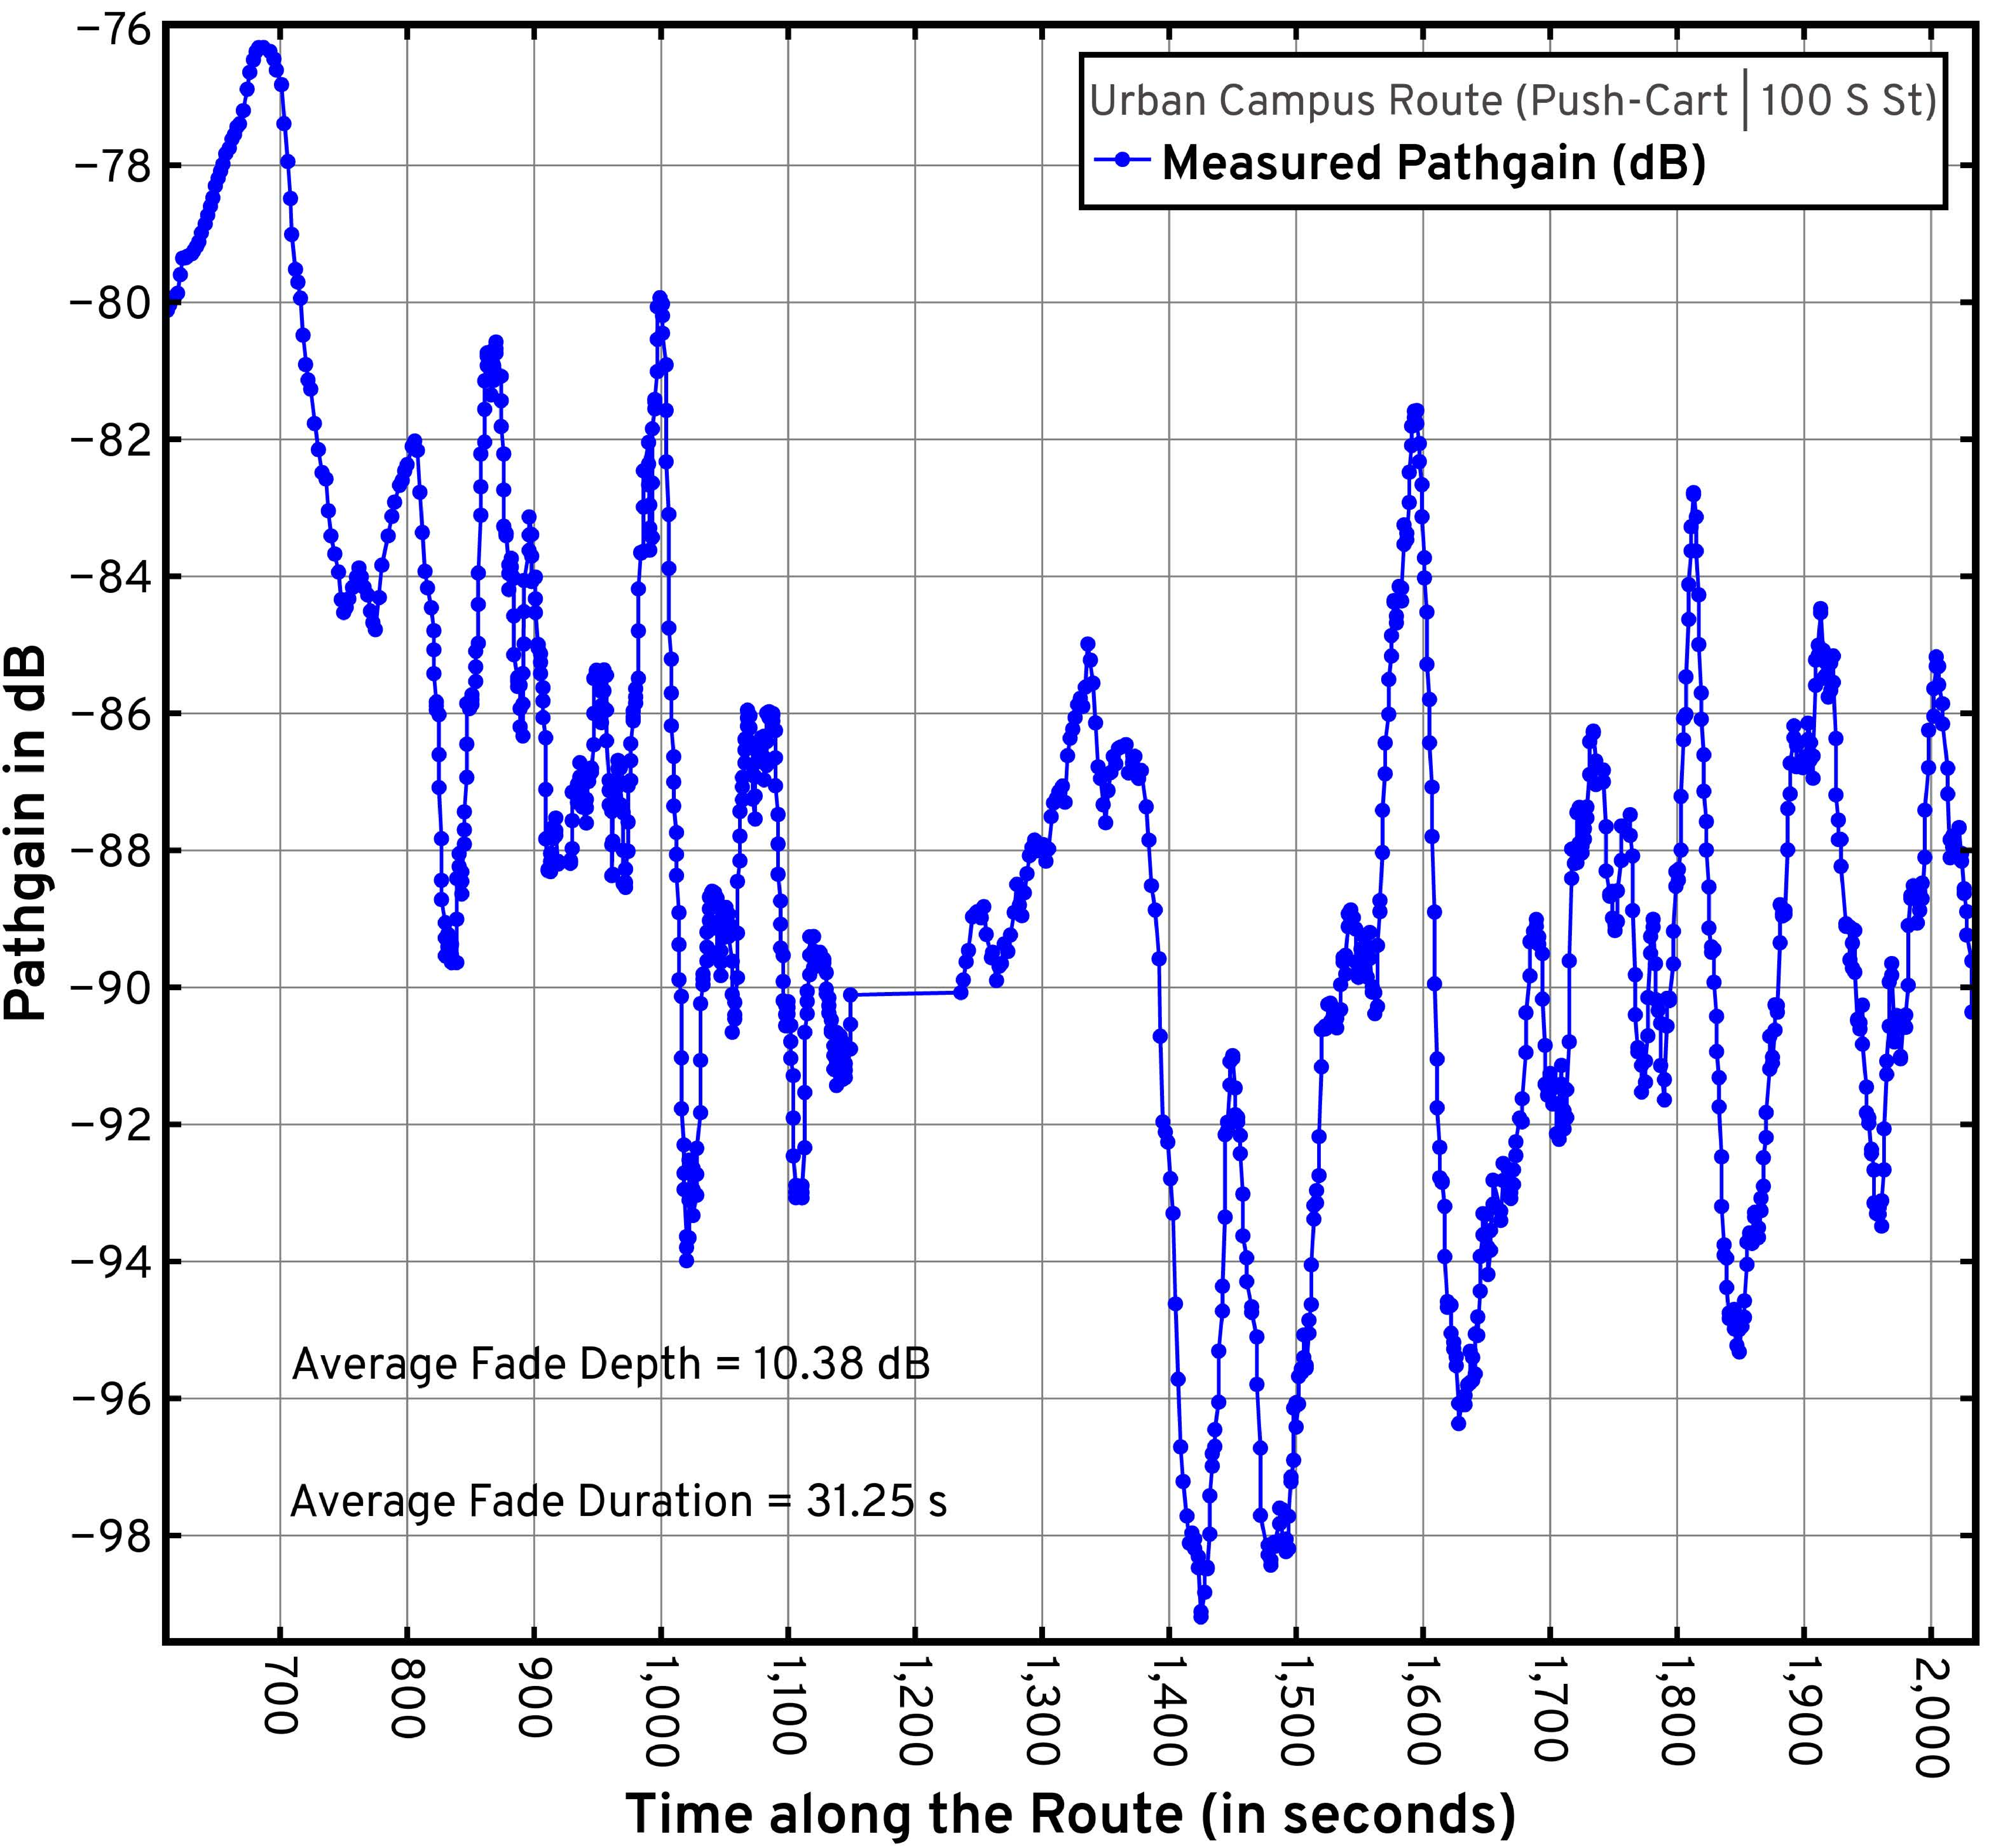
\includegraphics[width=1.0\linewidth]{figs/urban_campus_pathgain_vs_time.pdf}
         \caption{Urban Campus (100 S St)}
         \label{F10a}
     \end{subfigure}
     \begin{subfigure}{0.508\linewidth}
         \centering
         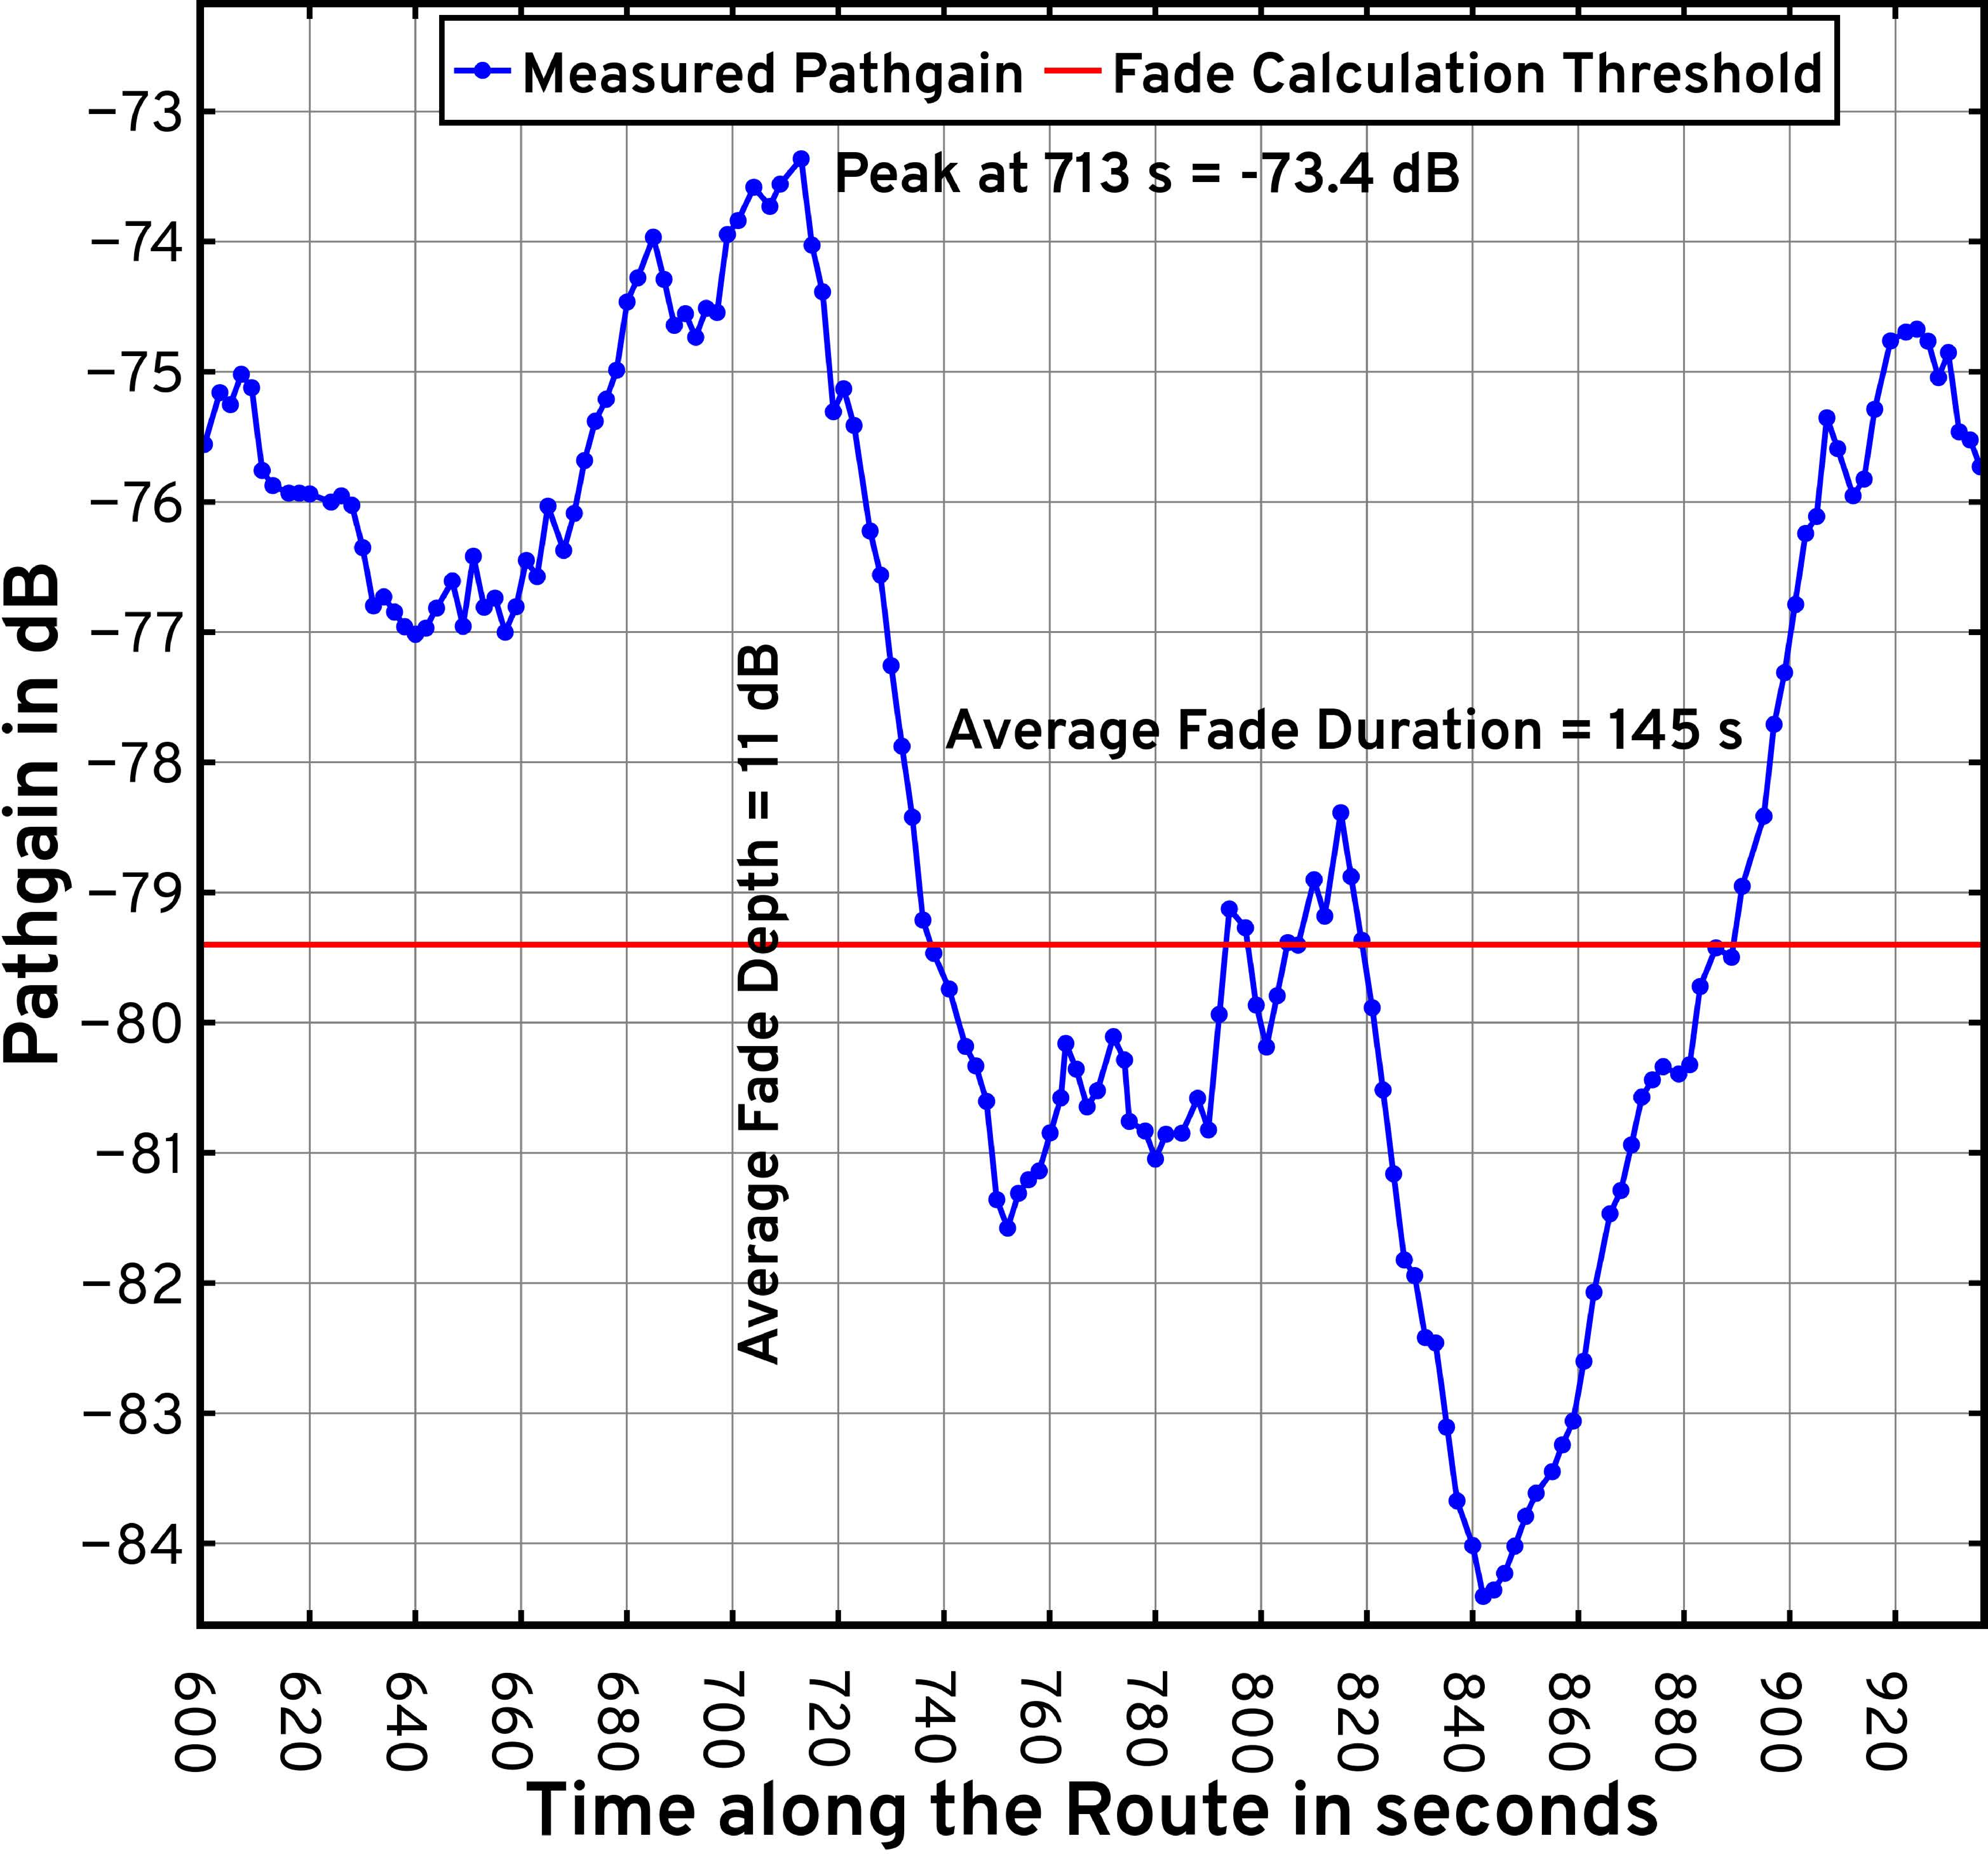
\includegraphics[width=1.0\linewidth]{figs/suburban_pathgain_vs_time.pdf}
         \caption{Suburban Neighborhood (S Wolcott St)}
         \label{F10b}
     \end{subfigure}
     \vspace{-8mm}
     \caption{The plots illustrating the small-scale fading effects (pathgain vs time) experienced by mmWave signals along routes dominated by dynamic blockages (pedestrians and moving/parked vehicles), i.e., the urban campus route around 100 S St (a) (Rx is on a push-cart) and the suburban neighborhood route around S Wolcott St (b) (Rx is again on a push-cart).}
     \label{F10}
\end{figure*}
\vspace{-3mm}

% Numerical evaluations II: Multipath clustering and Channel model validations
\section{Multipath Clustering and Channel Modeling}\label{S5}
In this section, using the multipath components extracted via the SAGE algorithm~\cite{SAGE}, we discuss multipath clustering studies involving the RMS delay- and direction-spreads, the cluster inter-arrival times, the cluster decay characteristics, and the cluster peak-power distributions. The Kolmogorov-Smirnov statistic enables experimental validations of widely-used mmWave channel models (SV~\cite{Indoor60G}, QD~\cite{QDC_NIST}, D$2$D~\cite{NISTModeling, D2DHumanBlockage}, and stochastic~\cite{Indoor60G}) by providing a measure of goodness between the empirical CDFs and the CDFs expected from these statistical channel models. Besides these multipath clustering analyses, illustrations of PDAPs shed novel insights on the temporal and spatial dispersion attributes of \SI{28}{\giga\hertz} signals; moreover, visualizations of the PDDPs and their associated normalized Doppler spectra facilitate investigations of the Doppler effects on \SI{28}{\giga\hertz} signals, which are particularly obvious in vehicular networks~\cite{DopplerHST}.
\vspace{-3mm}

% Concluding remarks and Future work
\section{Conclusion}\label{S6}
In this work, we discuss the design of a fully-autonomous beam-steering platform coupled with a sliding-correlator channel sounder, well-suited for mmWave V$2$X modeling. Corroborated onsite, this beam-steering system demonstrates superior performance vis-\`{a}-vis geo-positioning accuracy, alignment reliability, and tracking response times. Processing the recorded power delay profiles via custom noise elimination and thresholding heuristics, we perform pathloss evaluations against the popular $3$GPP TR$38.901$, ITU-R M$.2135$, METIS, and mmMAGIC outdoor urban micro- and macro-cellular standards. Herein, we demonstrate that such standards particularly fail to accurately model the pathloss versus log-distance behavior of \SI{28}{\giga\hertz} signals in V$2$X networks within urban, suburban, and foliage environments. Crucially, the continuous series of measurements facilitated by our design enables signal decorrelation studies under Tx-Rx distance, alignment accuracy, and relative velocity effects. Employing the SAGE algorithm, multipath clustering analyses -- centered around the Kolmogorov-Smirnov statistic -- facilitate empirical validations of the SV, QD, D$2$D, and stochastic channel models vis-\`{a}-vis cluster arrival and decay characteristics, cluster peak-power distributions, and RMS delay- and direction-spreads. Moreover, visualizations of the power delay angular profiles along various routes onsite enable analysis of temporal and spatial dispersion attributes of \SI{28}{\giga\hertz} signals along OLoS and NLoS links; visualizations of the power delay Doppler profiles and the associated normalized Doppler spectra permit investigations into the Doppler effects typically observed in vehicular networks. Finally, in addition to shadow-fading, this paper examines the small-scale fading properties of the obstructed signal, i.e. the average fade depth and the average duration under dynamic blockages (pedestrians and moving/parked vehicles) in vehicular communication applications (V$2$I/V$2$V).
\vspace{-3mm}

% References (main.bib)
\bibliographystyle{IEEEtran}
\bibliography{IEEEabrv,main}

\end{document}
% Content ends